%%%%%%%%%%%%%%%%%%%%%%%%%%%%%%%%%%%%%%%%%%%%%%%%%%%%%%%%%%%%%%%%%%%%%%%%%%%
\chapter{Methodology}
%%%%%%%%%%%%%%%%%%%%%%%%%%%%%%%%%%%%%%%%%%%%%%%%%%%%%%%%%%%%%%%%%%%%%%%%%%%

% Add these to your PREAMBLE (not inside the chapter):
% \usepackage{float}
% \usepackage{caption}

\hspace*{\parindent}This chapter discusses the research and development approach adopted in building the proposed system. It outlines the overall design framework, the mapping of objectives to specific methods, and the chosen software development life cycle model. The phases and activities of the development process are detailed, along with the system architecture and design considerations. By presenting the methodology, this chapter establishes how the study systematically progresses from planning to implementation, ensuring that the system meets both functional requirements and quality standards.
\vspace{5mm}

\section{Systems Analysis}

\subsection{Research and Development Approach}

\subsection{Overall Design}

\hspace*{\parindent}This project utilizes Agile-inspired approaches of continuous development and review. The iterative development approach is used whereby the capabilities of the system are improved iteratively through development, testing, and feedback loops. This approach ensures that the system developed is aligned with user expectations and meets the technical specifications.
\vspace{5mm}

\subsection{Phased Deployment Across Naga City}

\hspace*{\parindent}The project follows a phased approach for deployment across Naga City:
\vspace{5mm}

\begin{enumerate}
    \item \textbf{Phase 1 (Foundation):} Development of the main multi-tenant system with functionalities such as authentication, user management, program CRUD, simple registration, and calendar view in three pilot barangays.
    \item \textbf{Phase 2 (Operations):} Implementation of attendance tracking (QR capable), expense tracking, budget dashboard with automated calculations, PDF report generation, notifications, and Public Viewer in three barangays.
    \item \textbf{Phase 3 (Engagement):} Introduction of the Boses ng Kabataan feedback system with functionalities like resolutions tracking (with youth polling), document management, notifications management, and dark mode in five barangays.
    \item \textbf{Phase 4 (Scale):} Expansion to a full multi-tenant dashboard, federation analytics, and API access in mobile-friendly format across all barangays in Naga City.
    \item \textbf{Phase 5 (Optimize):} Performance optimization, advanced analytics, automated reporting, training documentation, and support portal.
\end{enumerate}
\vspace{5mm}

\subsection{Mapping of Objectives to Methods}

\begin{table}[H]
\centering
\caption{Mapping of Objectives to Methodology Components}
\label{tab:objectives-methods}
\begin{tabular}{|p{6cm}|p{8cm}|}
\hline
\textbf{Objective} & \textbf{Methodology Component} \\
\hline
1. Assess current SK program and participant management & Requirement collection using interviews, document analysis, and observation techniques in chosen barangays of Naga City \\
\hline
2. Create a generic web-based system & Agile software development using a multi-tenant design and concurrent database creation \\
\hline
3. Develop core modules (scheduling, registration, attendance, reports, feedback, resolution tracking, notification, document management) & Sprint planning including iteration coding based on functional dependency \\
\hline
4. Determine user-friendliness and satisfaction & User testing using TAM questionnaire for usability testing among stakeholders in Naga City \\
\hline
5. Evaluate processing speed, accuracy, accessibility & Performance testing following ISO 25010 guidelines \\
\hline
\end{tabular}
\end{table}
\vspace{5mm}

\section{Systems Design}

\subsection{Software Development Methodology}

\hspace*{\parindent}The proposed project uses the Agile SDLC because of its adaptability and incrementality. In Agile methodology, there can be a discrete development and testing of the system modules before integration, thus ensuring that any problems that exist can be easily detected and iterative improvements done based on user feedback. The use of the Agile method to develop IS in local governance has been reported in studies such as those by Padilla and Amar about barangay management systems. Scrum is used, which involves two-week sprints, stand-ups, sprint planning, and sprint retrospectives in order to stay aligned with the requirements of stakeholders in Naga City.
\vspace{5mm}

\subsection{Phases and Activities}

\hspace*{\parindent}The development process consists of the following phases:
\vspace{5mm}

\begin{enumerate}
    \item \textbf{Planning:} The definition of the system requirements is made possible by consultations with stakeholders from the SK sector and recommendations from the panel. Requirements are prioritized through the MoSCoW technique (Must have, Should have, Could have, Won't have).
    \item \textbf{Design:} Multi-tenant architecture is developed with emphasis on database design to ensure role-based security using Row-Level Security (RLS). Seven user interface designs are created to match the roles.
    \item \textbf{Development:} The system is developed iteratively, focusing on functional components in the following order: Authentication, Programs, Registration, Attendance, Expenses, Feedback, Resolution Tracker, Documents, Notifications, and Mobile Responsiveness.
    \item \textbf{Testing:} The testing process includes functional testing, usability testing, performance testing, security testing, and penetration testing for both web and mobile interfaces.
    \item \textbf{Deployment:} The system is deployed on Vercel to ensure web accessibility across devices.
    \item \textbf{Maintenance:} Maintenance activities include bug fixing, security patches, continuous feature enhancements, and ongoing user support.
\end{enumerate}
\vspace{5mm}

\subsection{Detailed System Design}

\subsubsection{Business Process Flow}

\begin{figure}[H]
    \centering
    
\includegraphics[width=0.90\textwidth,height=0.72\textheight,keepaspectratio]{figures/business_process_flow.png}
    \caption{Business Process Flow of KABISIG}
    \label{fig:business_process_flow}
\end{figure}

\hspace*{\parindent}This diagram shows the step-by-step process of how residents register and join programs in the KABISIG system. It begins with registration, which is reviewed by the Barangay Administrator. Approved residents receive a digital ID and gain access to programs, events, and announcements. Program registration also requires approval before participation. Attendance is tracked using QR codes, while program activities are monitored through budget checks, document processing, and committee oversight. After completion, residents submit feedback, which is turned into analytics dashboards summarizing engagement, budget use, attendance, and evaluation. Finally, reports and announcements are generated, with approved updates shared on Facebook.
\vspace{5mm}

\subsubsection{Data Flow Diagram}

\begin{figure}[H]
    \centering
    
\includegraphics[width=0.90\textwidth,height=0.62\textheight,keepaspectratio]{figures/1.png}
    \caption{Data Flow Diagram}
   \label{fig:dfd_context}
\end{figure}

\hspace*{\parindent}This diagram illustrates how different user groups interact with the KABISIG system. At the top level, the Super Admin (Federation President) manages system configuration, barangay administration, user accounts, federation reports, and audit logs. The Barangay Admin (Chairperson) accesses program details, budget information, documents, announcements, and compliance reports. The SK Officials (Kagawad, Secretary, Treasurer) handle attendance records, budget expenses, documents, feedback, assigned programs, and notifications. Meanwhile, Youth Constituents (residents) receive digital IDs, announcements, program information, and can register, give feedback, and respond to polls. Finally, Viewers (the public) have limited access, viewing announcements, transparency dashboards, and public reports.
\vspace{5mm}

        \begin{figure}[H]
   \centering
         
\includegraphics[width=0.90\textwidth,height=0.62\textheight,keepaspectratio]{figures/1.png}
\caption{Data Flow Diagram -- Level 1}
   \label{fig:dfd_level1}
\end{figure}

\hspace*{\parindent}This diagram presents the overall architecture of the KABISIG system, showing how different user roles interact with system modules and databases. The Super Admin oversees system configuration, account management, and audit logs, while the Barangay Admin manages programs, budgets, documents, and compliance reports. The SK Officials handle program schedules, attendance, feedback, and assigned activities. Youth Constituents register, attend programs, provide feedback, and receive digital IDs, while Viewers access public reports and transparency dashboards. The system is organized into six main modules: resident registration and user management, program and attendance management, financial and asset management, document and resolution management, analytics and reporting, and announcement and notification management. Each module connects to specific databases, such as user profiles, program records, attendance logs, feedback, budget, expenses, documents, and announcements.
\vspace{5mm}

\subsubsection{Swimlane Diagram}

\begin{figure}[H]
   \centering
    \includegraphics[width=0.90\textwidth,height=0.62\textheight,keepaspectratio]{figures/swim_lane.png}
    \caption{Swimlane Diagram of KABISIG System}
   \label{fig:swimlane}
\end{figure}

\hspace*{\parindent}The swimlane diagram illustrates the overall workflow of the KABISIG system by showing the responsibilities and interactions of the Youth Constituent, SK Official, KABISIG System, SK Treasurer, and SK Secretary across four major phases: Registration and Account Approval, Program Planning and Registration, Program Execution and Attendance, and Financial Reporting and Records Management. It demonstrates how each actor performs specific tasks, while the system automates processes such as account validation, QR code generation, attendance recording, notifications, report generation, and document management to ensure an organized, transparent, and efficient management of SK programs and services.
\vspace{5mm}

\subsection{Program Flow}

\subsubsection{Resident Registration and Approval}

\begin{figure}[H]
\centering
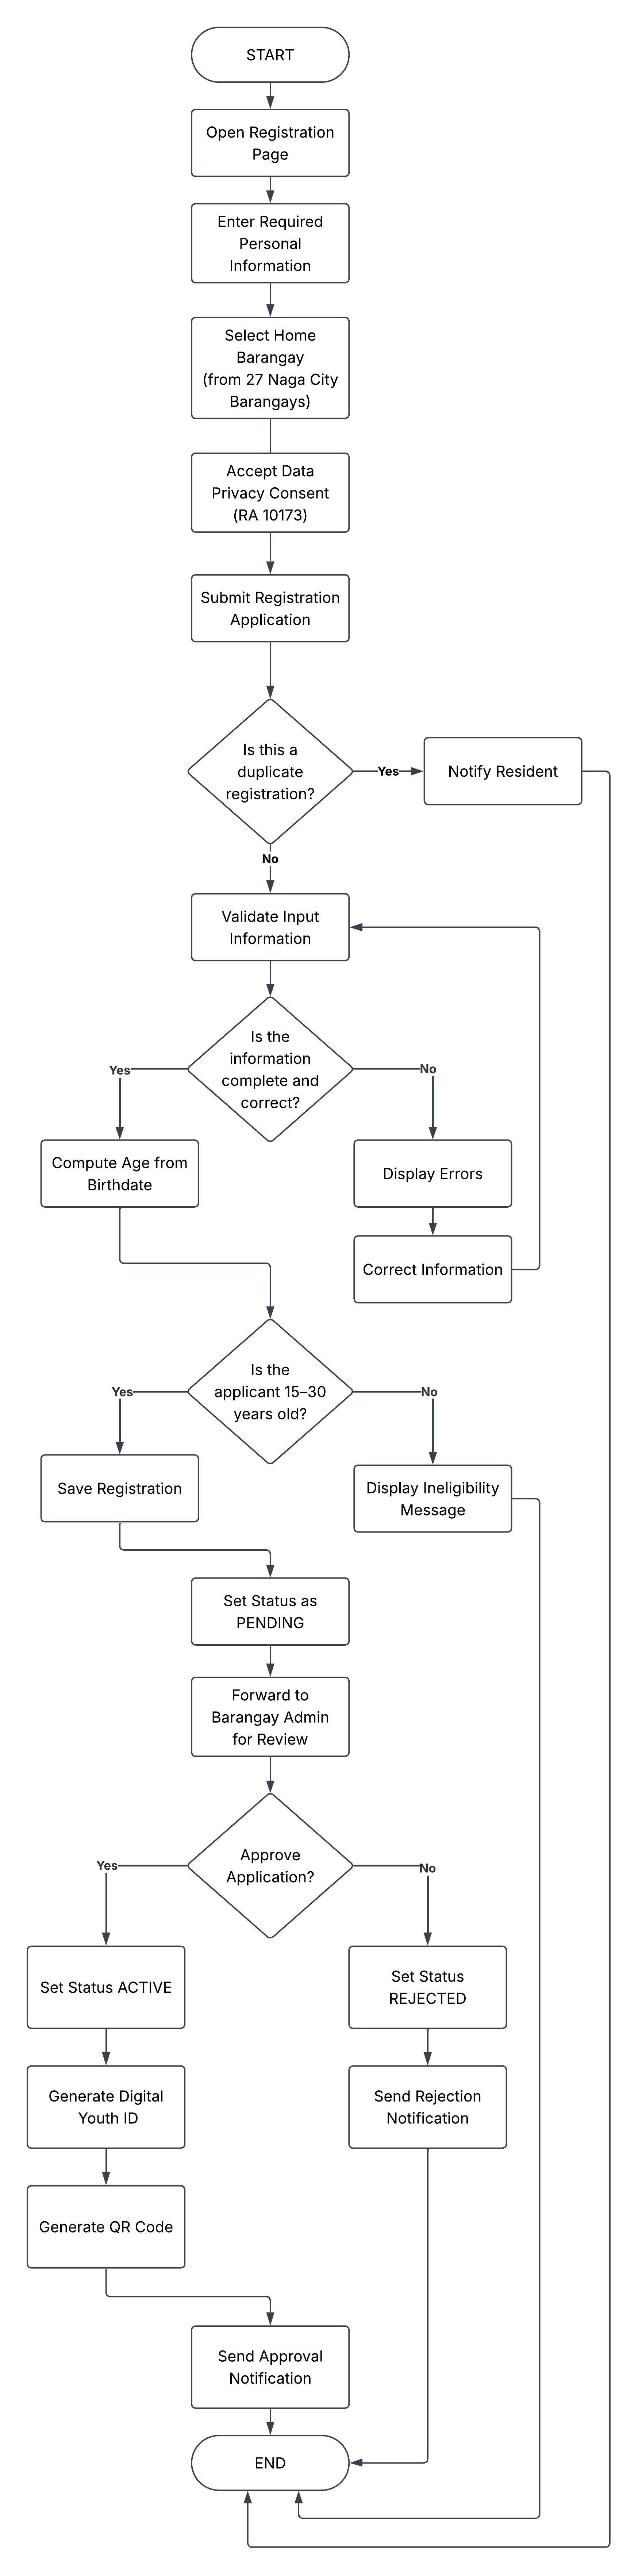
\includegraphics[width=0.90\textwidth,height=0.72\textheight,keepaspectratio]{figures/resident_registraion.png}
\caption{Resident Registration and Approval Activity Diagram}
\label{fig:registration-approval}
\end{figure}

\hspace*{\parindent}This diagram outlines the process of registering a youth constituent for a Digital Youth ID within the KABISIG system. The workflow begins when a youth constituent opens the registration page, enters personal information (full name, birthdate, address, school, guardian details, and other required fields), and submits the application. The system validates the input to check if it is complete and correct, and also validates the youth's age to ensure they are between 15 and 30 years old, as mandated by Republic Act No. 10742. If errors are found, the youth is prompted to correct them before the application proceeds.
\vspace{5mm}

\hspace*{\parindent}Once validated, the registration is saved with a status of pending and is reviewed by the Barangay Administrator or SK Secretary. At this stage, the administrator decides whether to approve or reject the application. Rejected applications trigger a notification to the youth, while approved applications result in the generation of a Digital Youth ID with a QR code for attendance tracking, along with an approval notification sent to the youth.
\vspace{5mm}

\subsubsection{Program Registration and QR Attendance}

\begin{figure}[H]
\centering
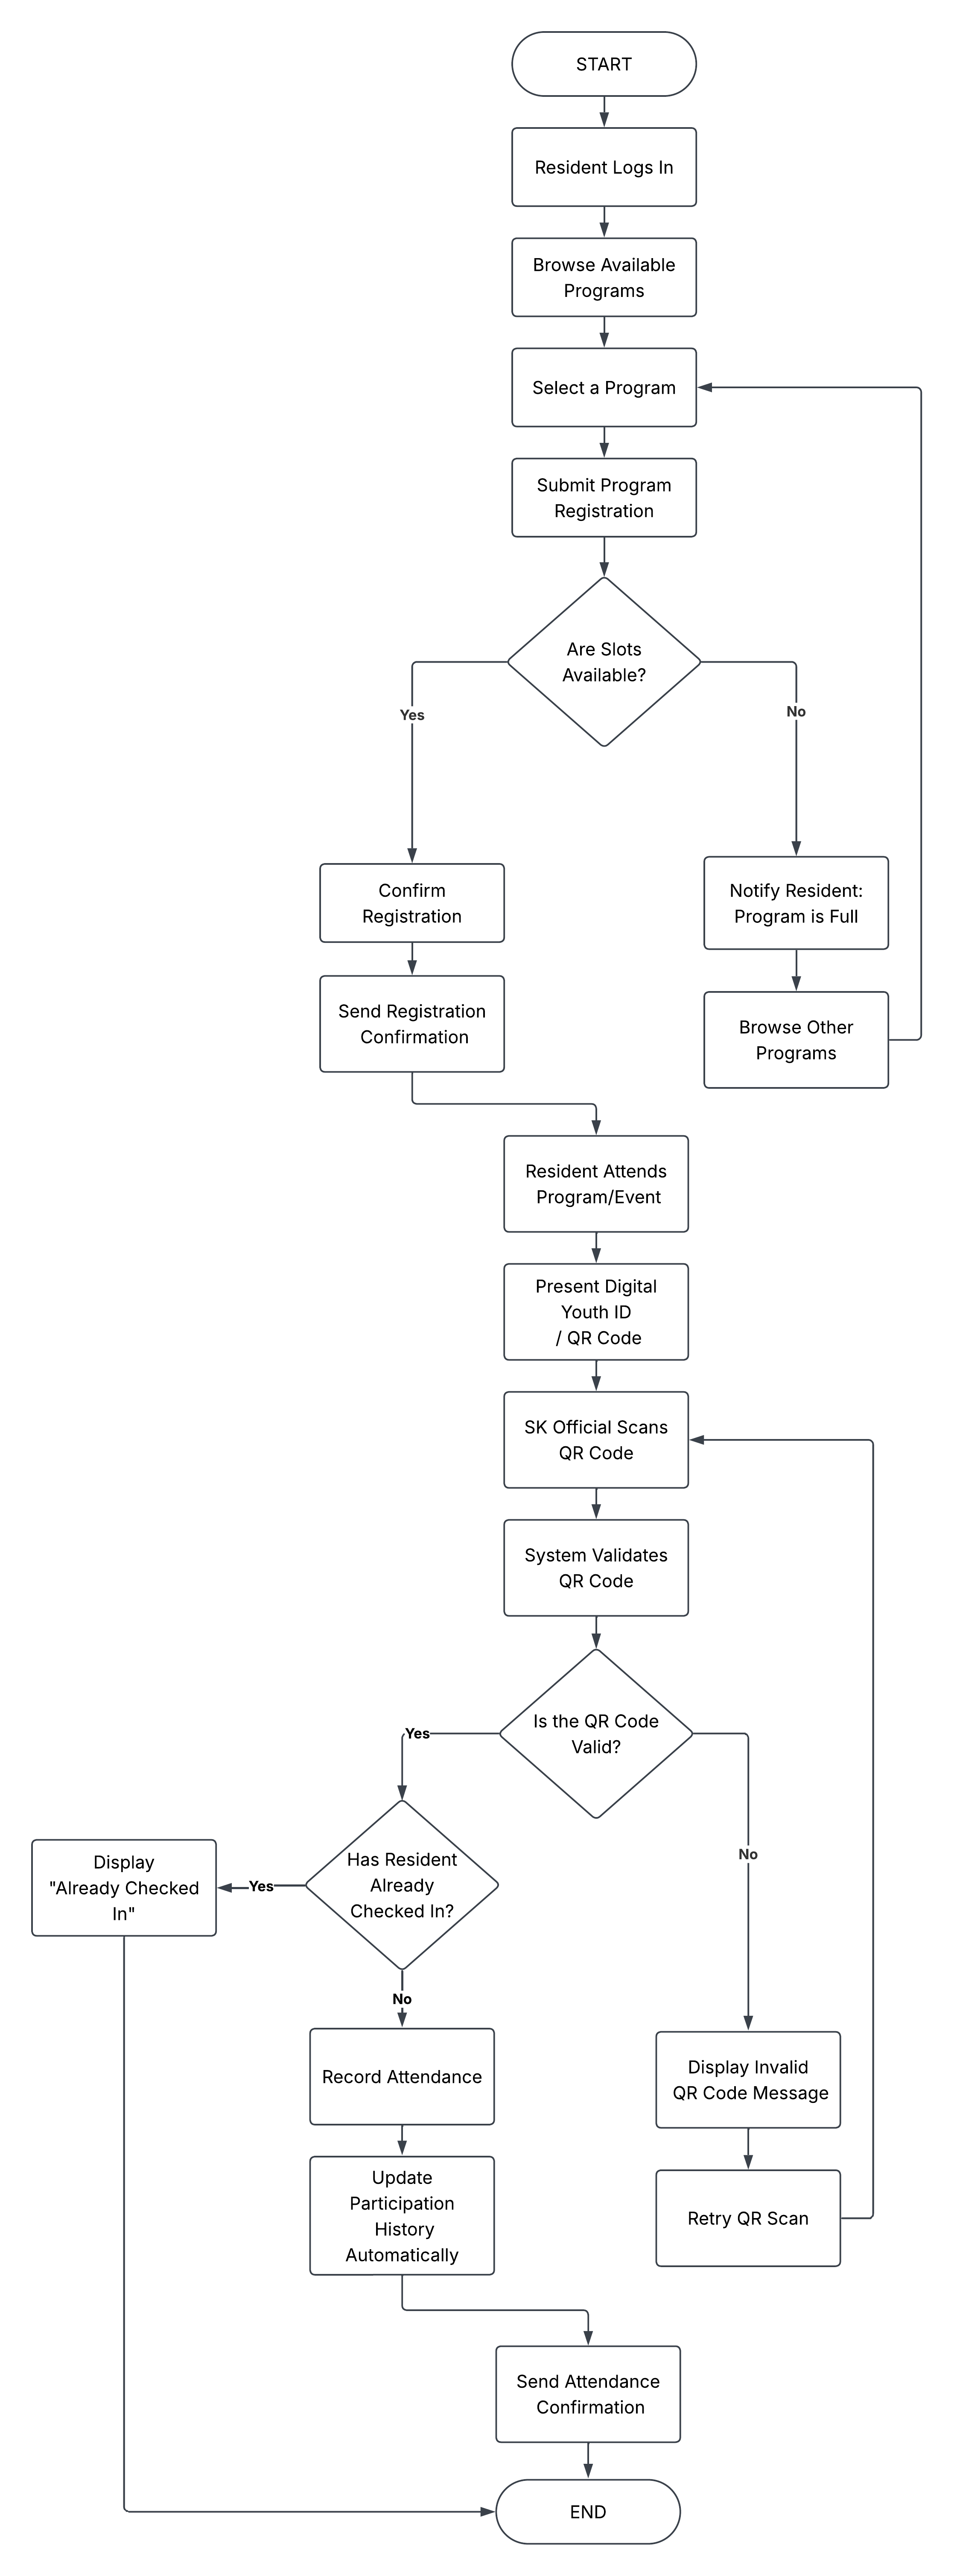
\includegraphics[width=0.90\textwidth,height=0.72\textheight,keepaspectratio]{figures/program_registration.png}
\caption{Program Registration and QR Attendance Activity Diagram}
\label{fig:program-registration}
\end{figure}

\hspace*{\parindent}This diagram shows the process of how residents register and attend programs within the KABISIG system. The workflow begins when a resident logs in, browses available programs, and selects one to join. The system checks slot availability before confirming registration. If slots are full, the resident is notified and directed back to browse other programs. Once registration is confirmed, the resident receives a notification and attends the event. Attendance is validated through QR code scanning, which the system uses to record participation. The resident's participation history is then updated automatically.
\vspace{5mm}

\subsubsection{Budget Management}

\begin{figure}[H]
    \centering
    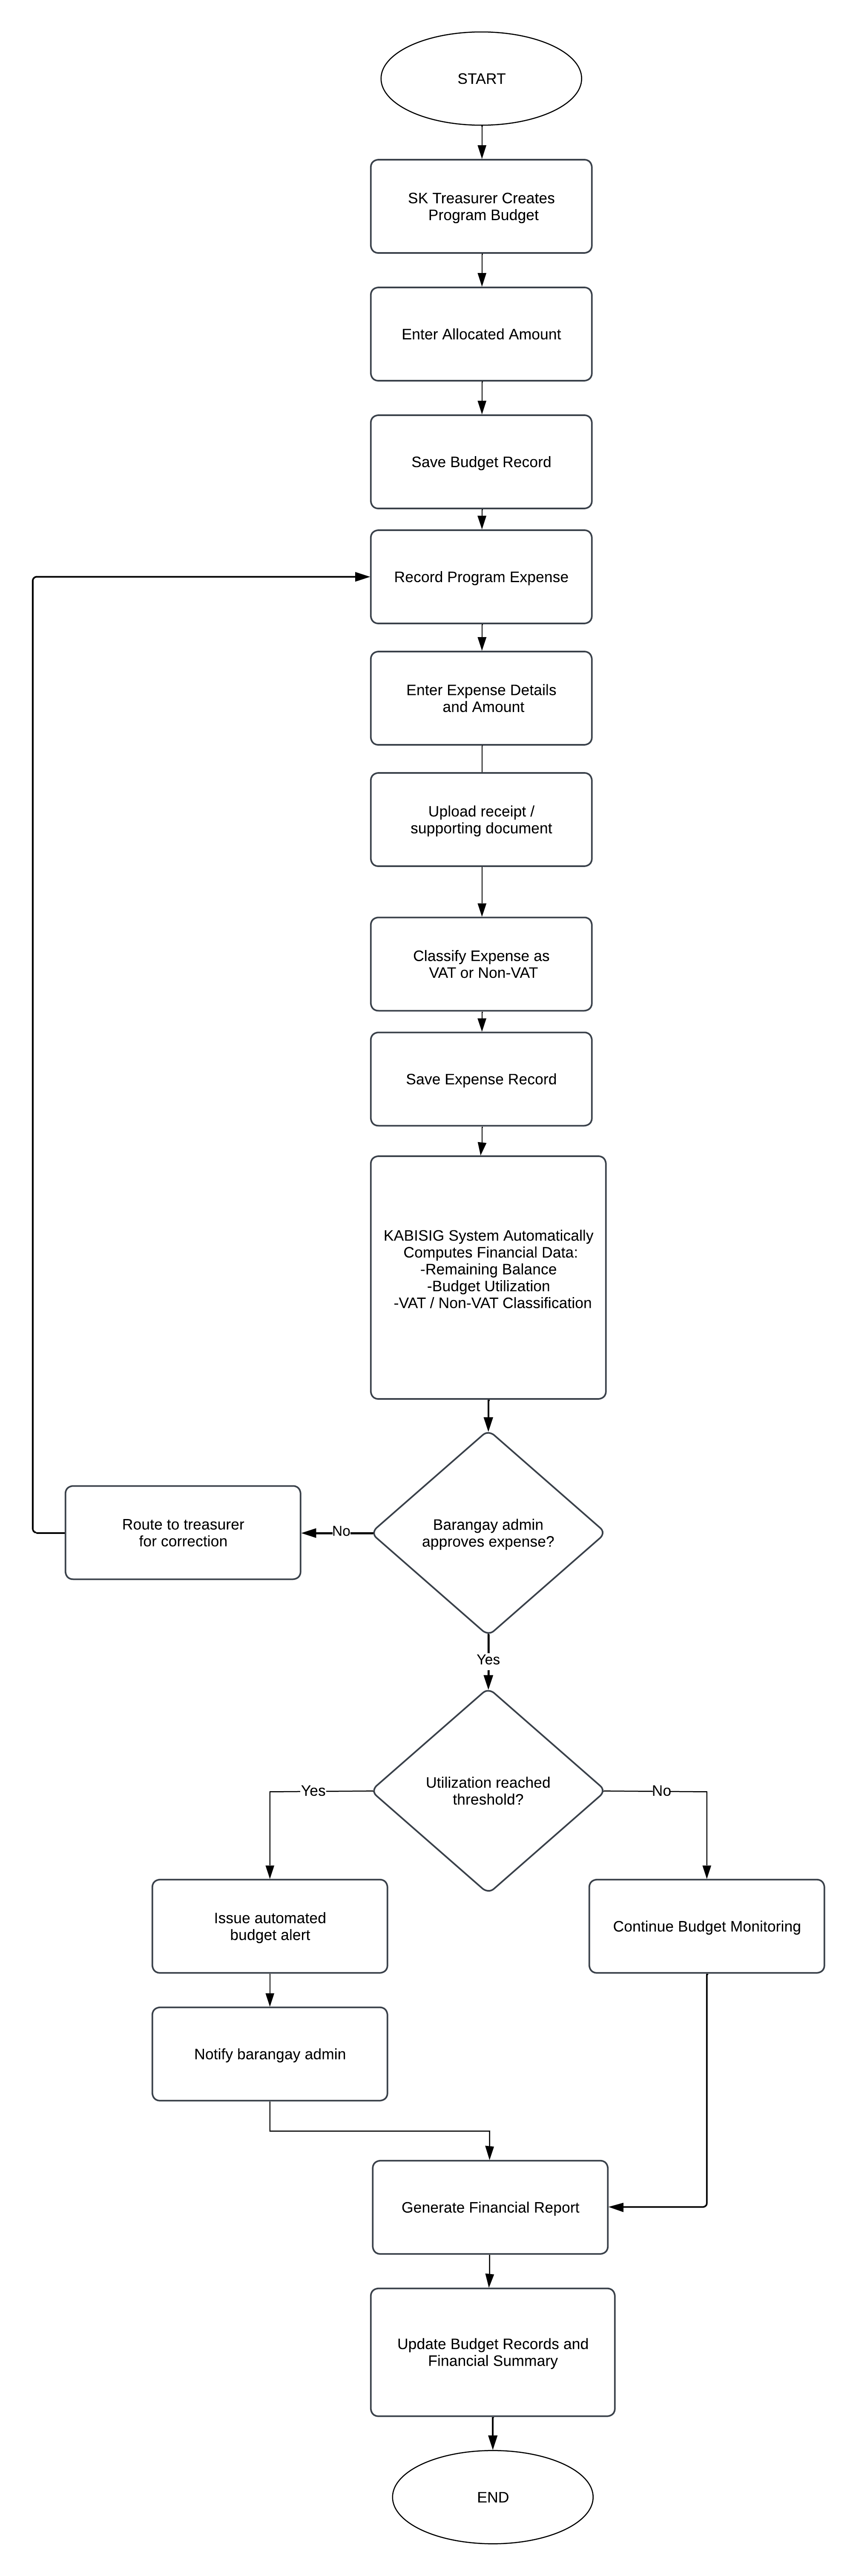
\includegraphics[width=0.90\textwidth,height=0.72\textheight,keepaspectratio]{figures/budget_management.png}
    \caption{Budget Management Activity Diagram}
    \label{fig:budget_management}
\end{figure}

\hspace*{\parindent}This diagram illustrates the process of managing program budgets within the KABISIG system. The workflow begins when the Treasurer creates a budget, enters the allocated amount, and saves the record. Expenses are then recorded, and the system automatically computes the remaining balance, budget utilization, and VAT or non-VAT classification. A decision point checks whether the budget has been exceeded. If not, the process continues normally. If exceeded, the system issues an automated budget alert to notify administrators. In both cases, the workflow leads to the generation of a financial report, which concludes the process.
\vspace{5mm}

\subsubsection{Document Approval Workflow}

\begin{figure}[H]
    \centering
    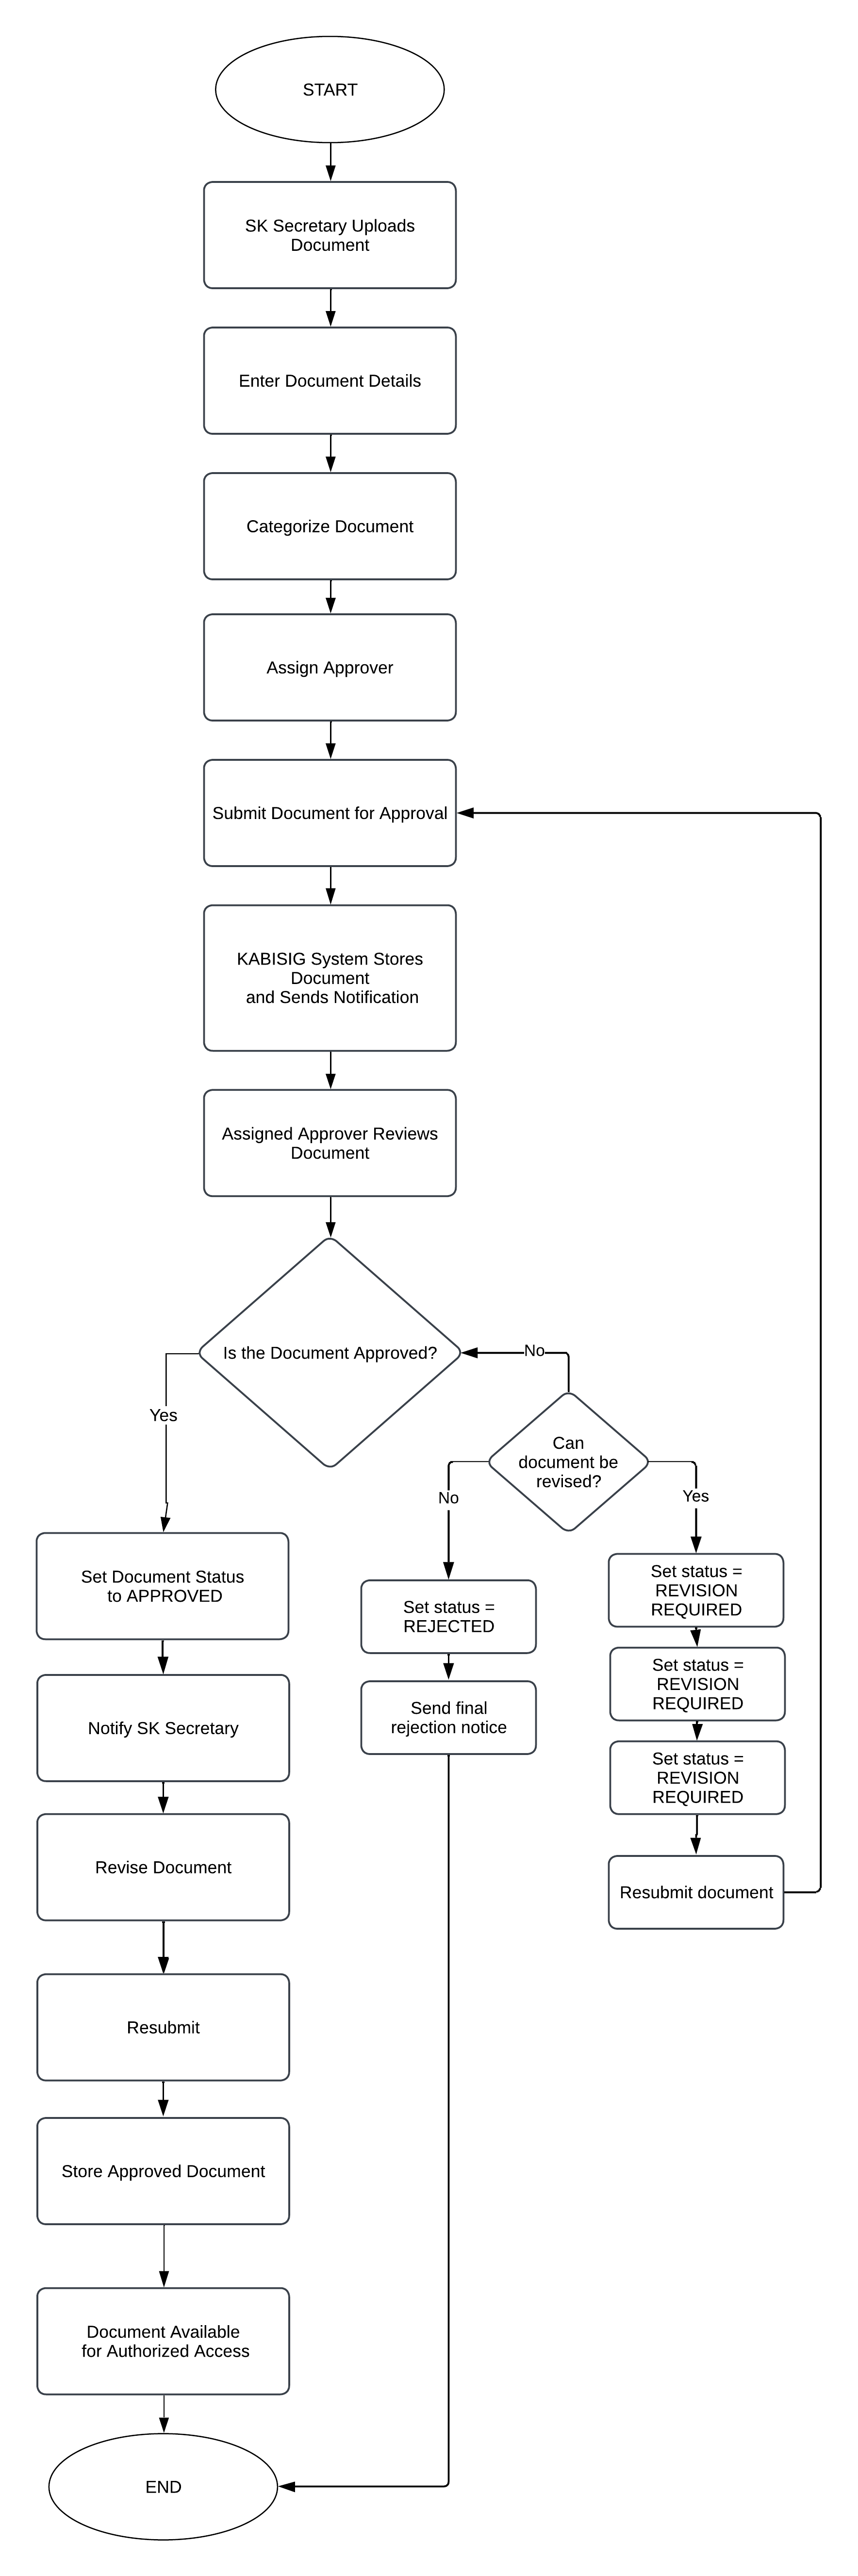
\includegraphics[width=0.90\textwidth,height=0.72\textheight,keepaspectratio]{figures/document_approval.png}
    \caption{Document Approval Workflow}
    \label{fig:document_approval}
\end{figure}

\hspace*{\parindent}This diagram shows the process of document approval within the KABISIG system. The workflow begins when the Secretary uploads a document, categorizes it, and assigns an approver. The approver is notified and reviews the document.
\vspace{5mm}

\subsubsection{Feedback and Automated Analytics}

\begin{figure}[H]
    \centering
    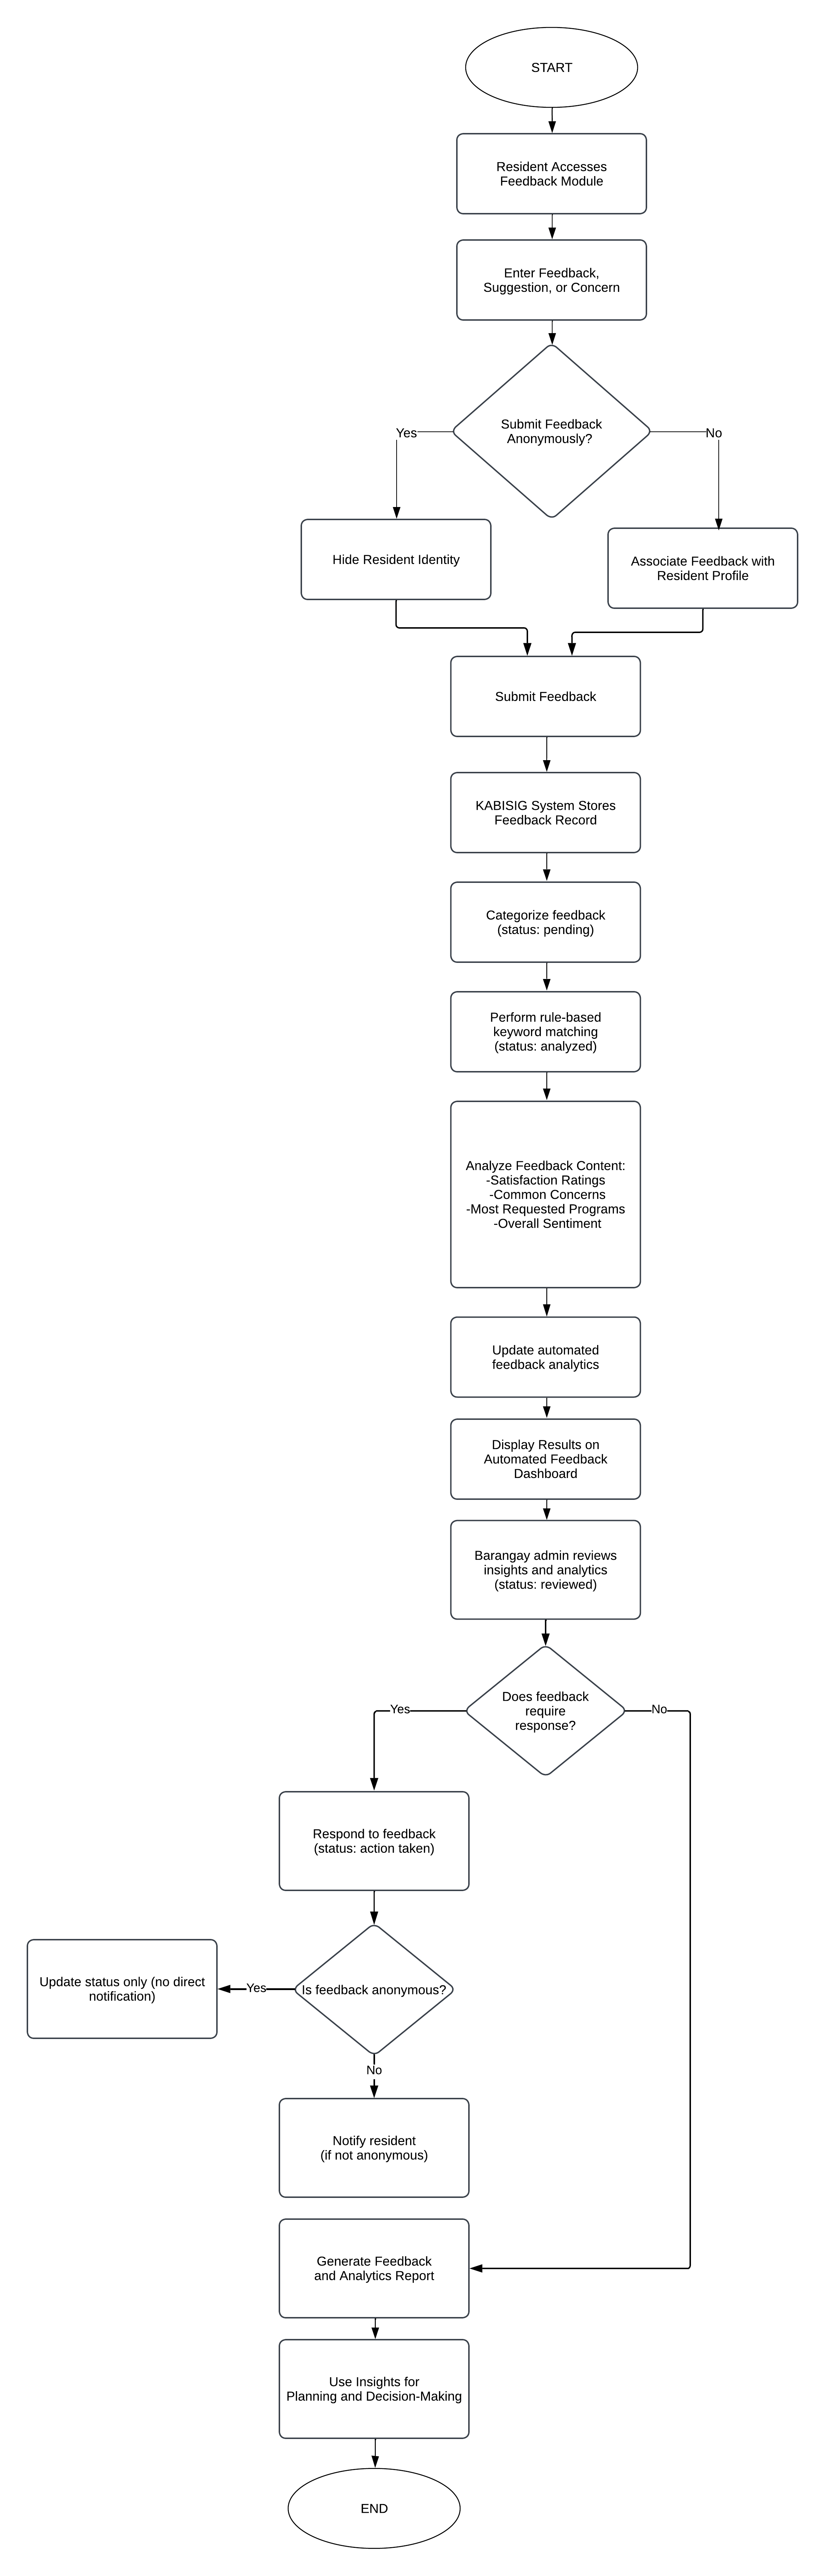
\includegraphics[width=0.90\textwidth,height=0.72\textheight,keepaspectratio]{figures/feedback_automated.png}
    \caption{Feedback and Smart Analytics Activity Diagram}
    \label{fig:feedback_analytics}
\end{figure}

\hspace*{\parindent}This diagram illustrates how resident feedback is collected and processed within the KABISIG system. The process begins when a resident submits feedback, which the system stores and categorizes. The feedback is then analyzed using rule-based keyword matching to update key indicators such as satisfaction ratings, common concerns, most requested programs, and overall sentiment. The results are displayed in an automated feedback dashboard, allowing administrators to review insights and generate reports. The process concludes with the reporting stage, ensuring that feedback is transformed into actionable information.
\vspace{5mm}

\subsubsection{Use Case Diagram}

\begin{figure}[H]
    \centering
    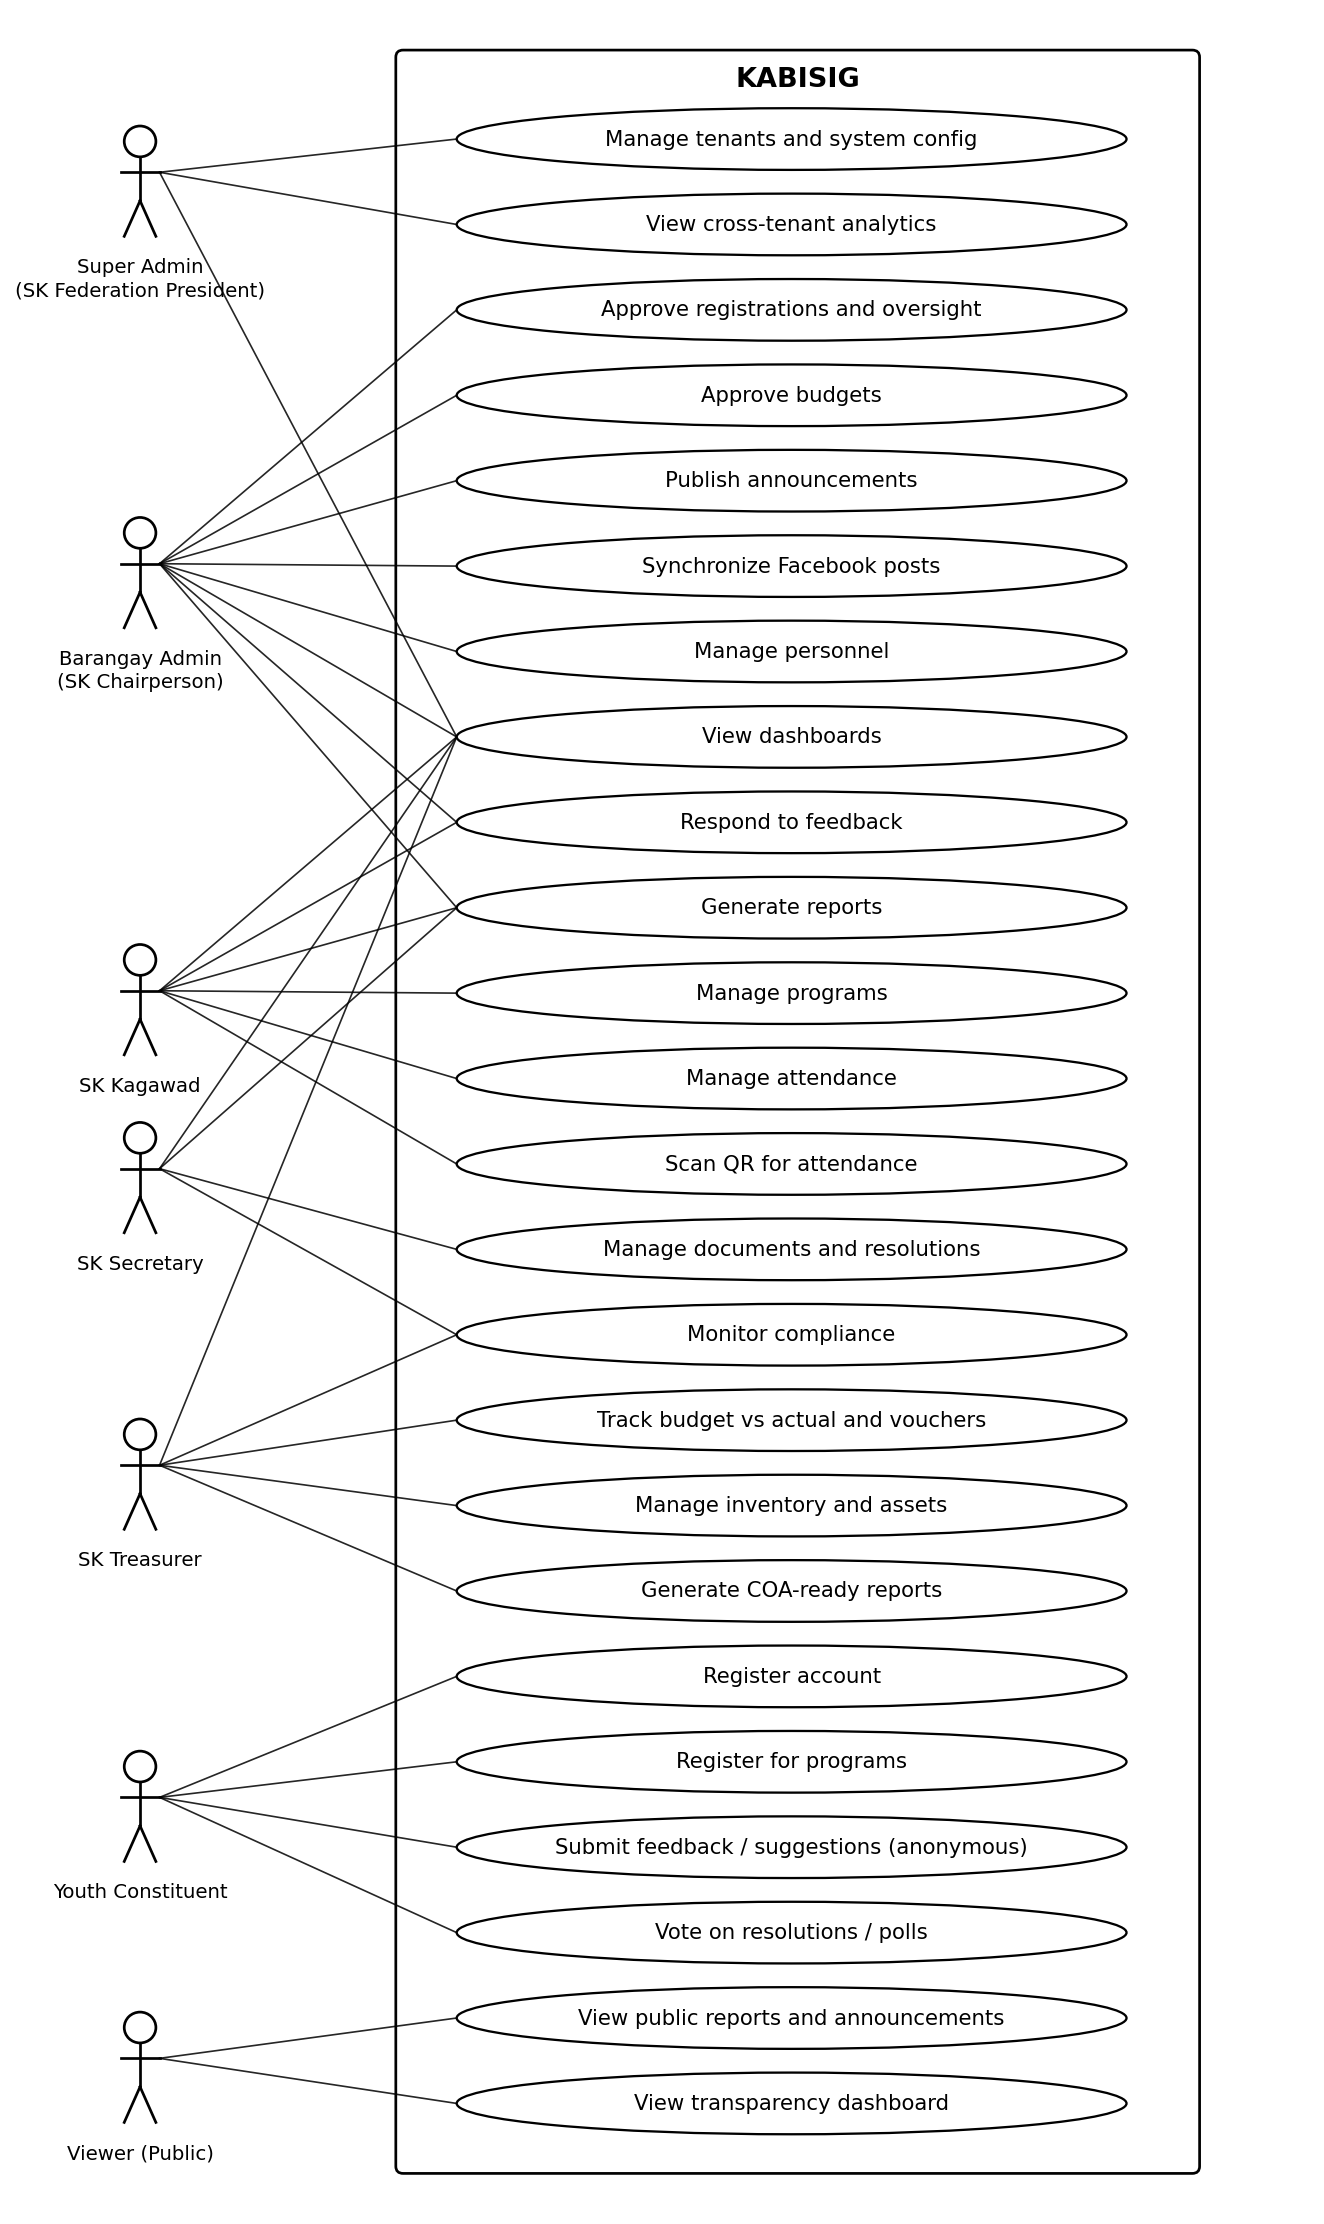
\includegraphics[width=0.90\textwidth,height=0.72\textheight,keepaspectratio]{figures/use_case.png}
    \caption{Use Case Diagram of KABISIG}
    \label{fig:use_case}
\end{figure}


\hspace*{\parindent}This diagram presents the different user roles and their interactions with the KABISIG system. On the administrative side, the Super Admin (Federation President) manages system configuration, personnel, committees, tenants, and cross-barangay analytics. The Barangay Admin (Chairperson) oversees resident profiles, program and event management, budgets, documents, resolutions, and announcements. The SK Officials (Kagawad, Secretary, Treasurer) support program operations, attendance recording, budget and expense management, and document handling. Youth Constituents register accounts, log in, join programs, record attendance via QR codes, submit feedback, and respond to polls. Viewers (public users) have limited access, focusing on announcements and public reports.
\vspace{5mm}

\subsubsection{Entity-Relationship Diagram}

\begin{figure}[H]
    \centering
    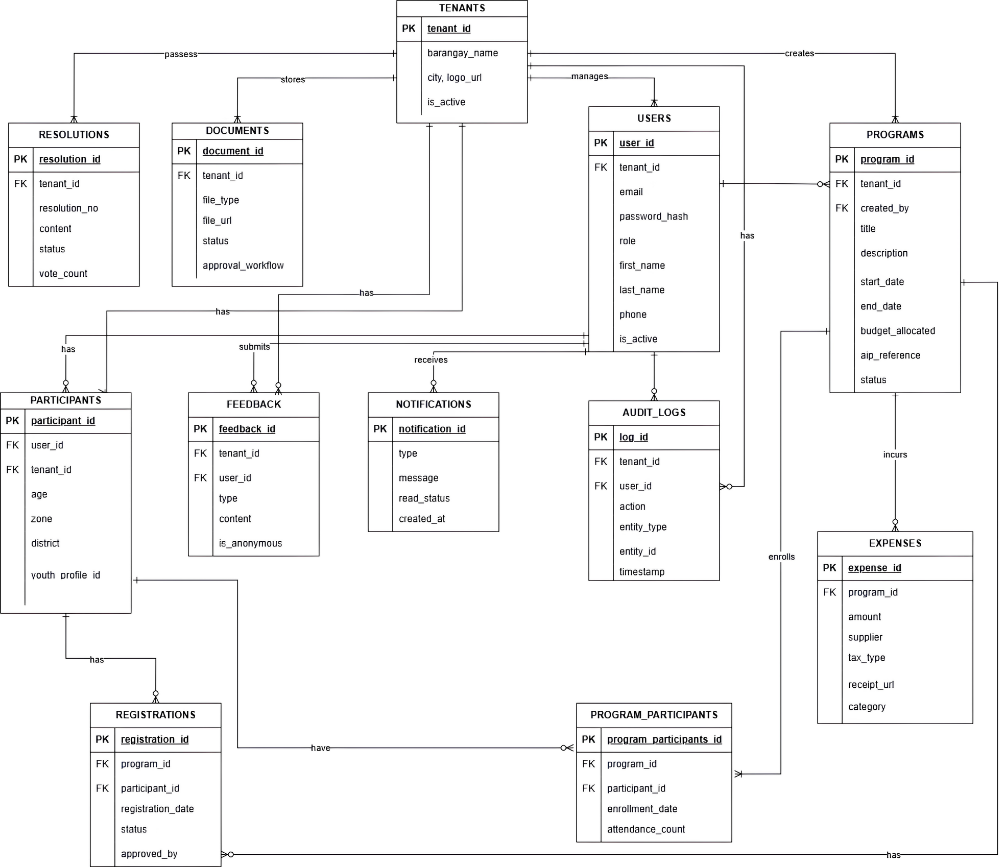
\includegraphics[width=0.90\textwidth,height=0.72\textheight,keepaspectratio]{figures/ERD.png}
    \caption{Entity-Relationship Diagram of KABISIG}
    \label{fig:erd}
\end{figure}

\hspace*{\parindent}The ERD includes the following core and additional entities required for the system's intelligent features:
\vspace{5mm}

\hspace*{\parindent}\textbf{Core Entities:}
\vspace{2mm}

\hspace*{\parindent}ROLES, USERS, BARANGAY, RESIDENT\_PROFILE, PROGRAM, PROGRAM\_REGISTRATIONS, ATTENDANCE, BUDGET, EXPENSE, INVENTORY, DOCUMENT, ANNOUNCEMENT, NOTIFICATIONS, FEEDBACK, POLL, POLL\_RESPONSE, COMMITTEE, COMMITTEE\_ASSIGNMENT, AUDIT\_LOGS
\vspace{5mm}

\hspace*{\parindent}\textbf{Additional Entities:}
\vspace{5mm}

\hspace*{\parindent}\textbf{SENTIMENT\_ANALYSIS}
\begin{itemize}
    \item sentiment\_analysis\_id (UUID, PK)
    \item feedback\_id (UUID, FK to FEEDBACK)
    \item sentiment\_label (VARCHAR 20) -- Positive, Neutral, Negative
    \item sentiment\_score (DECIMAL 3,2)
    \item category (VARCHAR 50)
    \item confidence (DECIMAL 3,2)
    \item response\_status (VARCHAR 20) -- Pending, Analyzed, Reviewed, Action Taken
    \item analyzed\_at (TIMESTAMP)
    \item created\_at (TIMESTAMP)
\end{itemize}
\vspace{5mm}

\hspace*{\parindent}\textbf{COMPLIANCE\_MONITORING}
\begin{itemize}
    \item compliance\_id (UUID, PK)
    \item tenant\_id (UUID, FK to TENANTS)
    \item compliance\_requirement (VARCHAR 255)
    \item compliance\_checklist (JSONB)
    \item report\_deadline (DATE)
    \item compliance\_status (VARCHAR 50) -- Pending, In Progress, Completed, Overdue
    \item submitted\_at (TIMESTAMP)
    \item submitted\_by (UUID, FK to USERS)
    \item approved\_by (UUID, FK to USERS)
    \item approved\_at (TIMESTAMP)
    \item reminder\_sent (BOOLEAN)
    \item created\_at (TIMESTAMP)
\end{itemize}
\vspace{5mm}

\hspace*{\parindent}\textbf{SOCIAL\_MEDIA\_POSTS}
\begin{itemize}
    \item social\_post\_id (UUID, PK)
    \item announcement\_id (UUID, FK to ANNOUNCEMENTS)
    \item tenant\_id (UUID, FK to TENANTS)
    \item facebook\_post\_id (VARCHAR 100)
    \item post\_content (TEXT)
    \item post\_status (VARCHAR 20) -- Draft, Scheduled, Posted, Failed
    \item scheduled\_time (TIMESTAMP)
    \item published\_time (TIMESTAMP)
    \item sync\_status (VARCHAR 20) -- Pending, Synced, Error
    \item error\_message (TEXT)
    \item created\_by (UUID, FK to USERS)
    \item created\_at (TIMESTAMP)
    \item updated\_at (TIMESTAMP)
\end{itemize}
\vspace{5mm}

\subsection{Development and Testing}

\subsubsection{Requirements Gathering}

\hspace*{\parindent}Requirements were collated through:
\vspace{5mm}

\begin{enumerate}
    \item Interviews with SK members such as the SK Chairperson, Kagawad, Secretary, and Treasurer to uncover issues and requirements in Naga City barangays.
    \item Review of previous reports, attendance sheets, word-processed plans, and governance documents.
    \item Analysis of existing resources including spreadsheets for tracking participants, Facebook/Messenger announcements, and manual filing systems for documents.
    \item Observation of manual processes during SK programs, SK meetings, and barangay council meetings.
    \item Review and gap analysis of panel recommendations for the current SK information systems.
\end{enumerate}
\vspace{5mm}

\subsection{Account Creation and Approval Workflow}

\hspace*{\parindent}Based on the requirements gathering activities, the following account creation and approval workflow was established:
\vspace{5mm}

\hspace*{\parindent}\textbf{Super Administrator:} The account is pre-created by the system developer during initial deployment and does not require approval from anyone, as no authority above the Super Administrator exists within the system. The SK Federation President receives credentials through a secure offline handoff and is required to change their password on first login.
\vspace{5mm}

\hspace*{\parindent}\textbf{Barangay Administrator (SK Chairperson):} The account is created directly by the Super Administrator through the Barangay Management module. The SK Chairperson does not self-register; instead, the Super Admin enters their details and the account is created with status = active immediately. The act of creation serves as the approval, reflecting the real-world process where SK Chairpersons are appointed by the SK Federation President.
\vspace{5mm}

\hspace*{\parindent}\textbf{SK Officials (Kagawad, Secretary, Treasurer):} Officials self-register through the public portal but cannot access the system until their account is approved by the Barangay Administrator. Upon registration, accounts are created with status = pending. The Barangay Admin receives a notification, reviews the applicant's details, and approves or rejects the registration through the User Management $\rightarrow$ Pending Accounts module. If approved, status changes to active and approved\_by is set to the Barangay Admin's user\_id.
\vspace{5mm}

\hspace*{\parindent}\textbf{Youth Constituents:} Youth self-register through the public youth portal, with accounts created in a pending state. The system validates age (15-30 years old) during registration. Barangay Administrators or assigned SK Officials review and approve youth registrations through the Youth Management $\rightarrow$ Pending Registrations module. Upon approval, the system automatically generates a Digital Youth ID with a QR code for attendance tracking.
\vspace{5mm}

\hspace*{\parindent}\textbf{Viewers:} Viewers do not require accounts. They access public-facing pages (Transparency Dashboard, Announcements, Program Schedules) without authentication. All public data is anonymized and aggregated for privacy compliance.
\vspace{5mm}

\hspace*{\parindent}This hierarchical approval workflow ensures that only verified barangay administrators manage SK operations, SK officials are legitimate council members appointed by their chairperson, youth constituents are verified residents within the 15-30 age range, and public transparency is maintained without creating barriers to access.
\vspace{5mm}

\section{Functional Requirements}

\subsection{System Features}

\hspace*{\parindent}The KABISIG system integrates multiple modules to support youth governance, program management, financial transparency, and community engagement. Each module provides specific functionalities that collectively ensure accountability, efficiency, and inclusivity.
\vspace{5mm}

\textbf{1. Resident Profiling and Participant Management}
\begin{itemize}
    \item \textbf{Resident Profiling} -- Keeps detailed records of residents' personal and community information.
    \item \textbf{Participant Registration, Verification, and Approval} -- Allows online sign-up with admin approval before access.
    \item \textbf{Demographic Categorization} -- Groups residents by status (e.g., student, scholar, employed, unemployed).
    \item \textbf{Zone- and District-Based Tracking} -- Organizes residents by geographic areas for easier monitoring.
    \item \textbf{Digital Resident ID Generation} -- Issues a unique digital ID for each approved participant.
    \item \textbf{QR Code Attendance Management} -- Records attendance using QR codes and prevents duplicate check-ins.
    \item \textbf{Beneficiary and Participation Monitoring} -- Tracks assistance received and participation history.
    \item \textbf{Automated Engagement Analytics} -- Calculates engagement scores using rule-based logic.
\end{itemize}
\vspace{5mm}

\textbf{2. Program, Event, and Community Governance Management}
\begin{itemize}
    \item \textbf{Program and Event Management} -- Enables creation, scheduling, and evaluation of activities.
    \item \textbf{Integrated Calendar Management} -- Centralizes schedules to avoid overlaps and conflicts.
    \item \textbf{Development Plan Monitoring} -- Monitors implementation of approved development plans.
    \item \textbf{Resolution and Ordinance Management} -- Handles drafting, approval, and archiving of official SK documents.
    \item \textbf{Committee and Responsibility Assignment} -- Assigns roles and responsibilities for projects and events.
    \item \textbf{Community Polling and Surveys} -- Collects opinions and votes from residents for decision-making.
    \item \textbf{Program Participation Monitoring} -- Tracks registrations, attendance, and completion of programs.
    \item \textbf{Automated Schedule Conflict Detection} -- Detects overlapping programs and schedule inconsistencies.
\end{itemize}
\vspace{5mm}

\textbf{3. Financial Transparency and Resource Management}
\begin{itemize}
    \item \textbf{Budget Allocation and Utilization Monitoring} -- Tracks how funds are assigned and spent for programs.
    \item \textbf{Automated Financial Computations} -- Calculates balances, utilization rates, and taxes automatically (VAT/Non-VAT).
    \item \textbf{Expense, Liquidation, and Receipt Management} -- Records and organizes financial transactions.
    \item \textbf{Budget Reversion Monitoring} -- Tracks unused funds available for reallocation or reversion.
    \item \textbf{Automated Budget Monitoring} -- Analyzes spending, detects overspending, and sends alerts.
    \item \textbf{Inventory and Asset Management} -- Keeps records of equipment, supplies, and other assets.
    \item \textbf{Asset Turnover Tracking} -- Monitors issuance, return, transfer, and disposal of assets.
    \item \textbf{Public Transparency Dashboard} -- Shows summarized financial data for public viewing.
\end{itemize}
\vspace{5mm}

\textbf{4. Document and Records Management}
\begin{itemize}
    \item \textbf{Centralized Document Repository} -- Stores all official documents securely in one place.
    \item \textbf{Document Categorization and Status Tracking} -- Organizes documents by type and monitors their progress.
    \item \textbf{Digital Approval Workflow} -- Routes documents electronically to designated signatories.
    \item \textbf{Automated PDF Report Generation} -- Creates reports like attendance sheets and financial summaries.
    \item \textbf{Automated Compliance Monitoring} -- Tracks pending approvals, overdue reports, and missing documents.
\end{itemize}
\vspace{5mm}

\textbf{5. Community Engagement and Feedback Management}
\begin{itemize}
    \item \textbf{Community Feedback Platform} -- Provides a platform for residents to share concerns and suggestions.
    \item \textbf{Suggestions and Concern Submission} -- Allows residents to submit requests and complaints.
    \item \textbf{Anonymous Feedback Support} -- Enables anonymous reporting to encourage honest participation.
    \item \textbf{Program and Project Evaluation} -- Collects participant ratings and feedback after activities.
    \item \textbf{Community Consultations and Surveys} -- Conducts surveys to support evidence-based planning.
    \item \textbf{Automated Feedback Analysis} -- Uses keyword-based (rule-based) classification to summarize feedback into concerns, requested programs, and sentiment.
\end{itemize}
\vspace{5mm}

\textbf{6. Analytics, Reporting, and Decision Support}
\begin{itemize}
    \item \textbf{Real-time Dashboards} -- Shows live summaries of registrations, attendance, budgets, and programs.
    \item \textbf{Program Performance Analytics} -- Measures participation, completion rates, satisfaction, and budget use.
    \item \textbf{Demographic and Beneficiary Analytics} -- Analyzes resident demographics and distribution of beneficiaries.
    \item \textbf{Attendance and Engagement Analytics} -- Identifies trends in participation and engagement levels.
    \item \textbf{Cross-Community Analytics} -- Compares performance and statistics across different barangays.
\end{itemize}
\vspace{5mm}

\textbf{7. Notification and Communication Management}
\begin{itemize}
    \item \textbf{Announcements and Broadcasts} -- Publishes official announcements and advisories.
    \item \textbf{Program and Event Reminders} -- Sends reminders before, during, and after activities.
    \item \textbf{Registration and Approval Notifications} -- Notifies users about registration status and approvals.
    \item \textbf{Calendar-Based Alerts} -- Generates alerts based on scheduled events and deadlines.
    \item \textbf{Compliance Reminders} -- Reminds personnel about upcoming reports, approvals, and compliance tasks.
\end{itemize}
\vspace{5mm}

\textbf{8. Organization and Personnel Management}
\begin{itemize}
    \item \textbf{Organizational Structure Management} -- Maintains the SK organizational chart and hierarchy.
    \item \textbf{Personnel Profiles and Role Management} -- Manages user accounts, roles, and access permissions.
    \item \textbf{Committee and Responsibility Management} -- Assigns committees and tracks responsibilities.
    \item \textbf{Personnel Attendance Monitoring} -- Records attendance during meetings and official activities.
    \item \textbf{Performance and Compliance Monitoring} -- Tracks personnel participation and compliance with tasks.
    \item \textbf{Administrative Oversight Dashboard} -- Provides administrators with organization-wide monitoring tools.
\end{itemize}
\vspace{5mm}

\textbf{9. Social Media Integration and Public Information}
\begin{itemize}
    \item \textbf{Official Facebook Page Integration} -- Connects the system to the SK's official Facebook page.
    \item \textbf{Automatic Announcement Synchronization} -- Publishes approved announcements directly to Facebook.
    \item \textbf{Scheduled Facebook Posting} -- Allows announcements to be posted automatically at set times.
    \item \textbf{Auto-generated Facebook Posts} -- Formats posts with event details, images, and QR codes.
    \item \textbf{Public Information Synchronization} -- Ensures consistency of public announcements between KABISIG and Facebook.
    \item \textbf{Post Status Tracking} -- Monitors posts with status: Draft, Scheduled, Posted, Failed.
\end{itemize}
\vspace{5mm}

\subsubsection{Sprint Planning}

\begin{table}[H]
\centering
\caption{Sprint Planning Phases}
\label{tab:sprint-planning}
\small
\begin{tabular}{|p{2.5cm}|p{1.5cm}|p{4cm}|p{5.5cm}|}
\hline
\textbf{Phase} & \textbf{Duration} & \textbf{Focus} & \textbf{Key Deliverables} \\
\hline
Phase 1: Planning and Documentation & Months 1--2 & Planning the project, identifying the system requirements, performing the analysis and designing of the system. & Completion of system requirements, scope and limitations, definition of user roles, use case scenarios, database design, UI/UX prototyping, system architecture design, project documentation and development plan. \\
\hline
Phase 2: Foundation Development & Month 3 & Designing the architecture and functionalities of the system. & Authentication processes, role based authorization, multi-tenancy, user management, database development, initial system interface, and web responsive design. \\
\hline
Phase 3: Core Operations Development & Month 4 & SK management functionality implementation. & Youth profiling, participant registration, program management, calendar management, attendance management, expense tracking, budgeting and simple report generation. \\
\hline
Phase 4: Governance and Engagement Features & Month 5 & Designing the modules to provide transparency and youth engagement. & Feedback management system for Boses ng Kabataan, issue management, youth survey, document and record management, notifications and public viewing capabilities. \\
\hline
Phase 5: Analytics and System Integration & Month 6 & Adding advanced functionalities and enhancements of the system. & Dashboards analytics, federation level analytics, automated reports, mobile responsiveness and API services. \\
\hline
Phase 6: Testing, Deployment, and Optimization & Month 7 & System testing, refinement, and preparation for deployment. & Functional testing, usability testing, User Acceptance Testing (UAT), security testing, performance tuning, bug fixing, user feedback driven improvements, user documentation and training material development. \\
\hline
\end{tabular}
\end{table}
\vspace{5mm}

\subsection{Version Control}

\hspace*{\parindent}The process utilizes Git version control which allows tracking changes made to the code, collaboration between developers, and reverting to a reliable version whenever necessary. Branch protection policies, pull request reviews, and continuous integration pipelines via GitHub Actions in total provide for the high-quality and stable nature of the code.
\vspace{5mm}

\subsection{Testing and Evaluation Procedures}

\subsubsection{Types of Testing}

\hspace*{\parindent}\textbf{Functional Testing:} Evaluation will cover CRUD operations, internal reports, RBAC, multi-tenancy, document approval process, notification functionality, and the precision of budget computations. Such approach is typical for software testing according to ISO 25010 and will be used to evaluate similar barangay information systems.
\vspace{5mm}

\hspace*{\parindent}\textbf{Usability Testing:} The usability evaluation will focus on the ease of navigation for the SK representatives and youth users in both the web and mobile versions of the system in terms of success rate of performing such tasks as creating programs, registration, giving feedback, and uploading documents. In order to assess the user satisfaction level, Technology Acceptance Model (TAM) and the Unified Theory of Acceptance and Use of Technology (UTAUT) will be used.
\vspace{5mm}

\hspace*{\parindent}\textbf{Performance Testing:} Evaluation will include real-time data processing, load time less than 2 seconds, API response time less than 500 ms, PDF creation time, and notification dispatch latency.
\vspace{5mm}

\hspace*{\parindent}\textbf{Security Testing:} Evaluation will include server-side security, RBAC, enforcement of RLS policies, data encryption, protection against penetration, and document access management. This corresponds to ISO/IEC 27001:2022 requirements.
\vspace{5mm}

\hspace*{\parindent}\textbf{Cross-Browser and Mobile Compatibility Testing:} Evaluation will include functional tests, layout consistency, and responsiveness in such popular browsers as Chrome, Firefox, Edge, Safari for desktop users and iOS Safari, Android Chrome for mobile users without the need for developing a dedicated app.
\vspace{5mm}

\subsubsection{Evaluation Criteria and Metrics}

\hspace*{\parindent}The system was evaluated using a five-point Likert scale based on:
\vspace{5mm}

\hspace*{\parindent}\textbf{ISO 25010 Software Quality Model:}
\begin{itemize}
    \item Functional Suitability
    \item Usability
    \item Performance Efficiency
    \item Reliability
    \item Security
\end{itemize}
\vspace{5mm}

\hspace*{\parindent}\textbf{Technology Acceptance Model (TAM):}
\begin{itemize}
    \item Perceived Usefulness (PU)
    \item Perceived Ease of Use (PEOU)
    \item Behavioral Intention to Use
    \item Actual System Use
\end{itemize}
\vspace{5mm}

\hspace*{\parindent}\textbf{Unified Theory of Acceptance and Use of Technology (UTAUT):}
\begin{itemize}
    \item Performance Expectancy
    \item Effort Expectancy
    \item Social Influence
    \item Facilitating Conditions
\end{itemize}
\vspace{5mm}

\hspace*{\parindent}\textbf{Custom Engagement Metrics:}
\begin{itemize}
    \item Monthly Active Users (MAU): Target $\geq$ 60\%
    \item Program Registration Rate: Target $\geq$ 90\%
    \item Attendance Rate: Target $\geq$ 75\%
    \item Feedback Submission Rate: Target $\geq$ 40\%
    \item SK Official Adoption Rate: Target $\geq$ 80\%
    \item Document Processing Time: Target $\leq$ 50\% reduction vs. manual
    \item Budget Reporting Accuracy: Target $\geq$ 98\%
\end{itemize}
\vspace{5mm}

\subsection{Implementation and Deployment Plan}

\subsubsection{Deployment Environment}

\hspace*{\parindent}Vercel is a tool used to deploy websites with automatic optimization of performance, serverless hosting, and secured handling of environment variables. The system is mobile responsive, allowing use of all features on any mobile web browser available without having to install another application. Supabase manages hosting of PostgreSQL with automatic backups, point in time recovery, row level security, real time databases, and geographical redundancy.
\vspace{5mm}

\subsubsection{User Training and Documentation}

\hspace*{\parindent}Users were oriented through:
\vspace{5mm}

\begin{enumerate}
    \item Organized system demonstrations for SK officials across Naga City barangays
    \item Step-by-step system usage guides for each user role
    \item Video tutorials for youth self-registration, feedback submission, and document upload
    \item Administrator documentation for tenant management, RBAC configuration, and document approval workflow setup
    \item SK Secretary/Treasurer-specific guides for document management and financial reporting
    \item Super Administrator training for cross-barangay analytics interpretation
\end{enumerate}
\vspace{5mm}

\subsubsection{Maintenance and Future Enhancements}

\hspace*{\parindent}The system is adaptable for future modifications:
\vspace{5mm}

\begin{itemize}
    \item Sophisticated analysis and advanced reporting on budget and program outcomes
    \item Email and SMS notification dissemination
    \item Enhanced mobile-responsive interface features
    \item Reinforced data protection, backup, and recovery protocols
    \item Interoperability APIs for national government database integration
    \item Integration with Naga City government digital services
\end{itemize}
\vspace{5mm}

\subsection{Summary}

\hspace*{\parindent}The methodology ensures that the project, KABISIG, uses an agile approach in accordance with internationally approved evaluation standards. The system thus increases its usefulness in solving operational challenges of the Sangguniang Kabataan program and participants in an effective manner. The step-by-step approach allows systematic validation at each phase while incorporating feedback from SK officials, and youth participants.
\vspace{5mm}

\subsection{User Interface and System Screens}

\hspace*{\parindent}The KABISIG system features a clean, modern, and mobile-responsive user interface designed to provide an intuitive experience across all user roles. The interface follows a consistent design language with the KABISIG color palette (Deep Blue \#1a237e, Vibrant Red \#d32f2f, White \#ffffff, and Gold \#fdd835) and a minimalist, government-appropriate aesthetic. Each screen is designed with the user's role and tasks in mind, ensuring efficient navigation and task completion.
\vspace{5mm}

\hspace*{\parindent}\textbf{Note:} The data presented in all screenshots are sample/placeholder data used for demonstration purposes only. They do not represent actual SK records, financial transactions, or personal information of any barangay, official, or youth constituent.
\vspace{5mm}

\subsubsection{Public Screens and Authentication}

\hspace*{\parindent}The public-facing screens provide unauthenticated users with access to system information and registration capabilities. The Public Transparency Portal allows citizens to view SK financial data, budget utilization, and program expenditures. This screen displays key metrics including city youth demographics, total federation budget, and total disbursed funds with utilization percentage. The Municipal Public Auditing Desk provides detailed expense tracking with transaction details, supplier information, and tax classifications.
\vspace{5mm}

\begin{figure}[H]
\centering
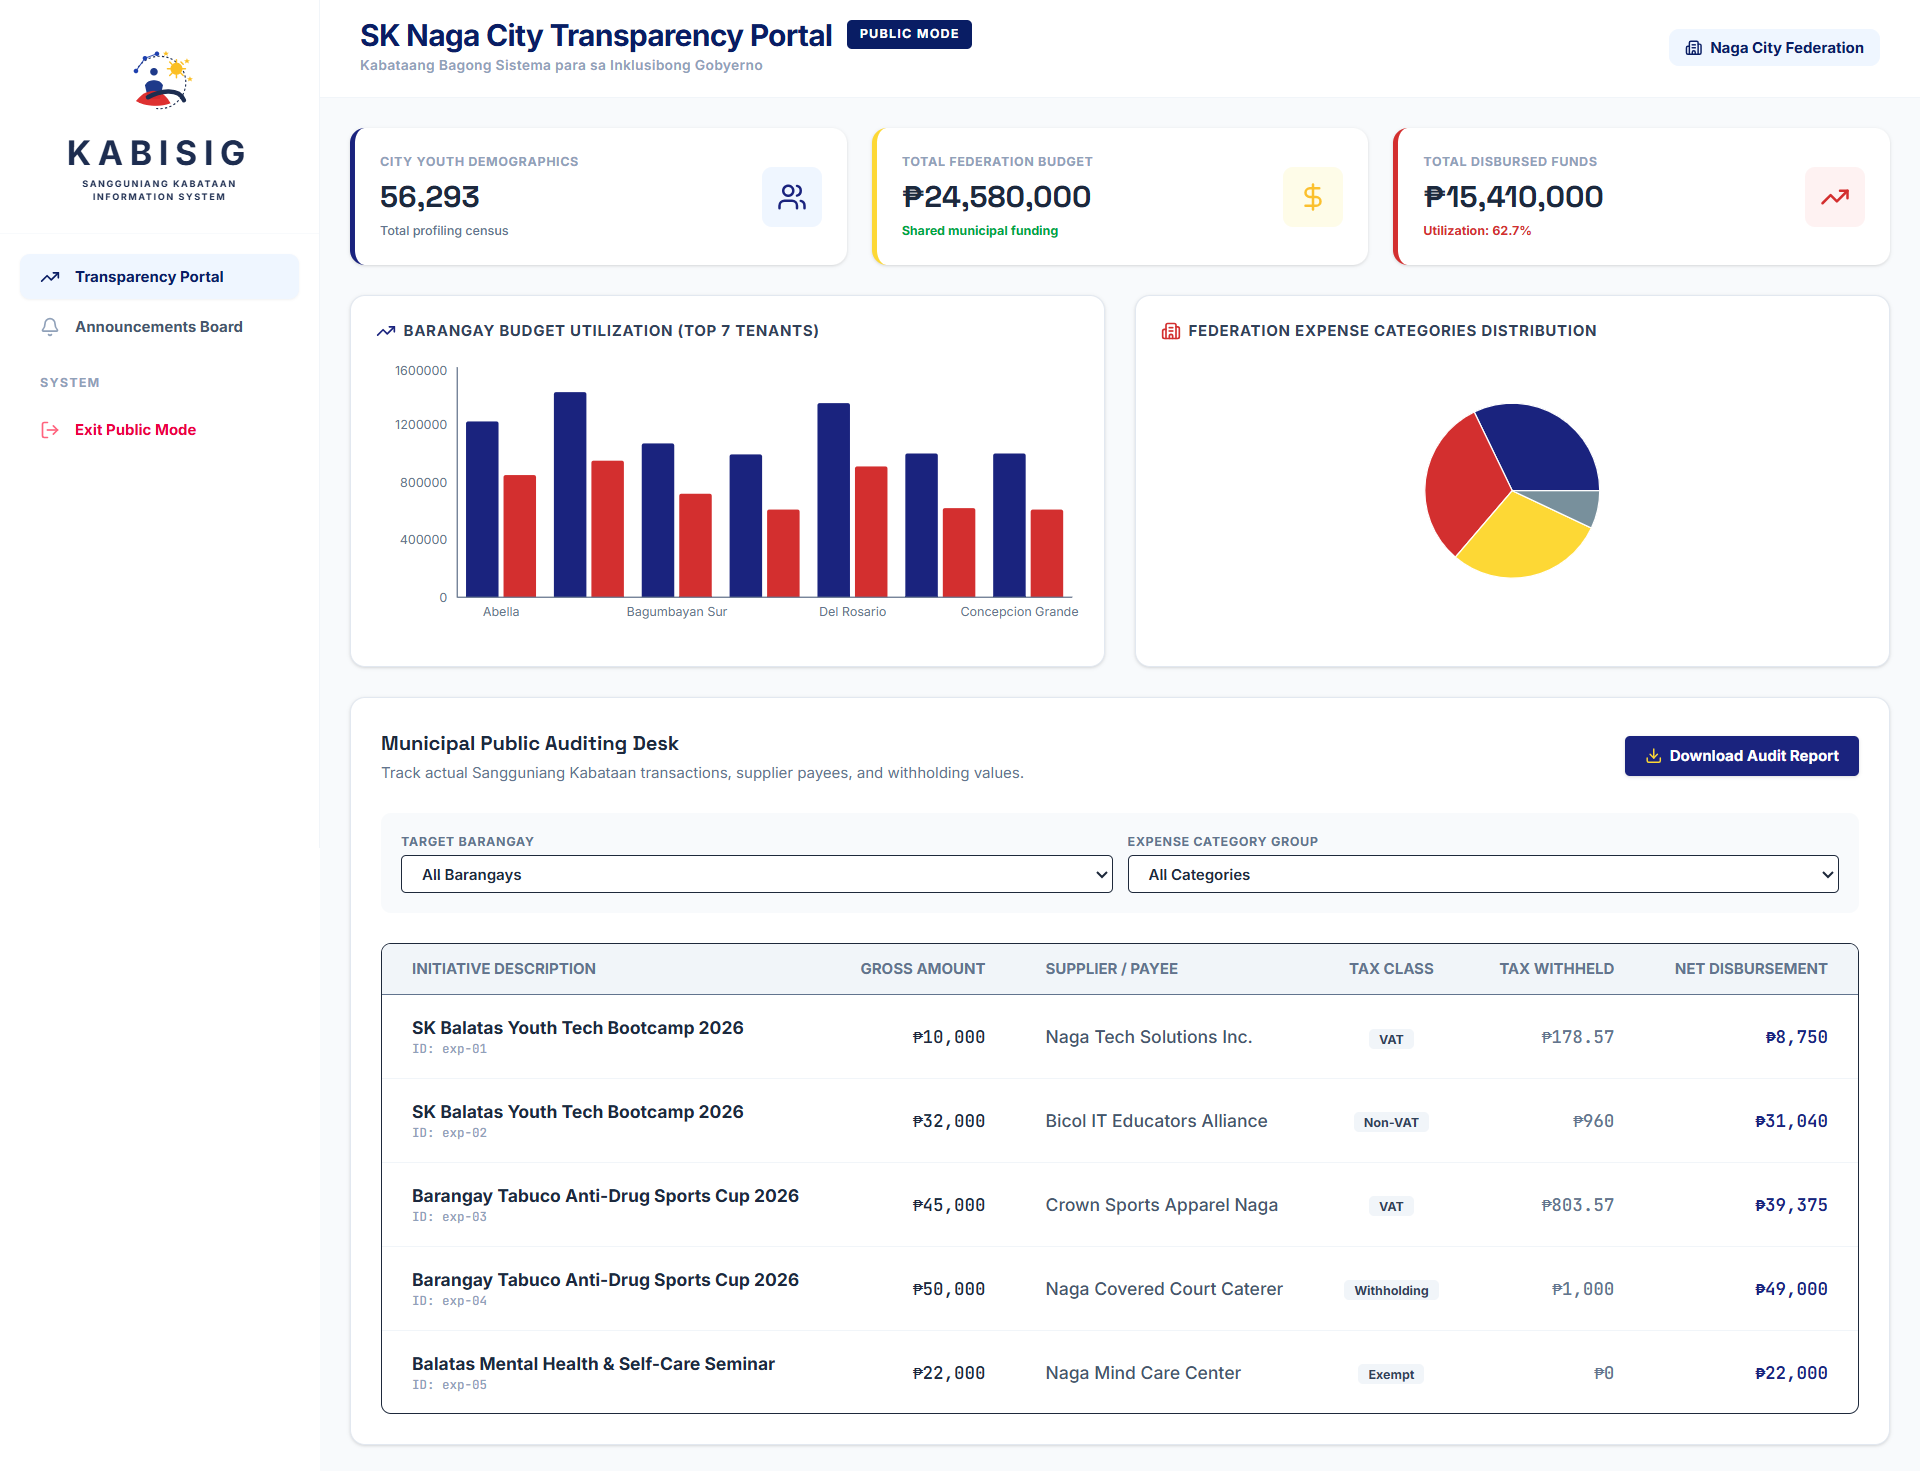
\includegraphics[width=0.45\textwidth]{figures/transparency_portal1.png}
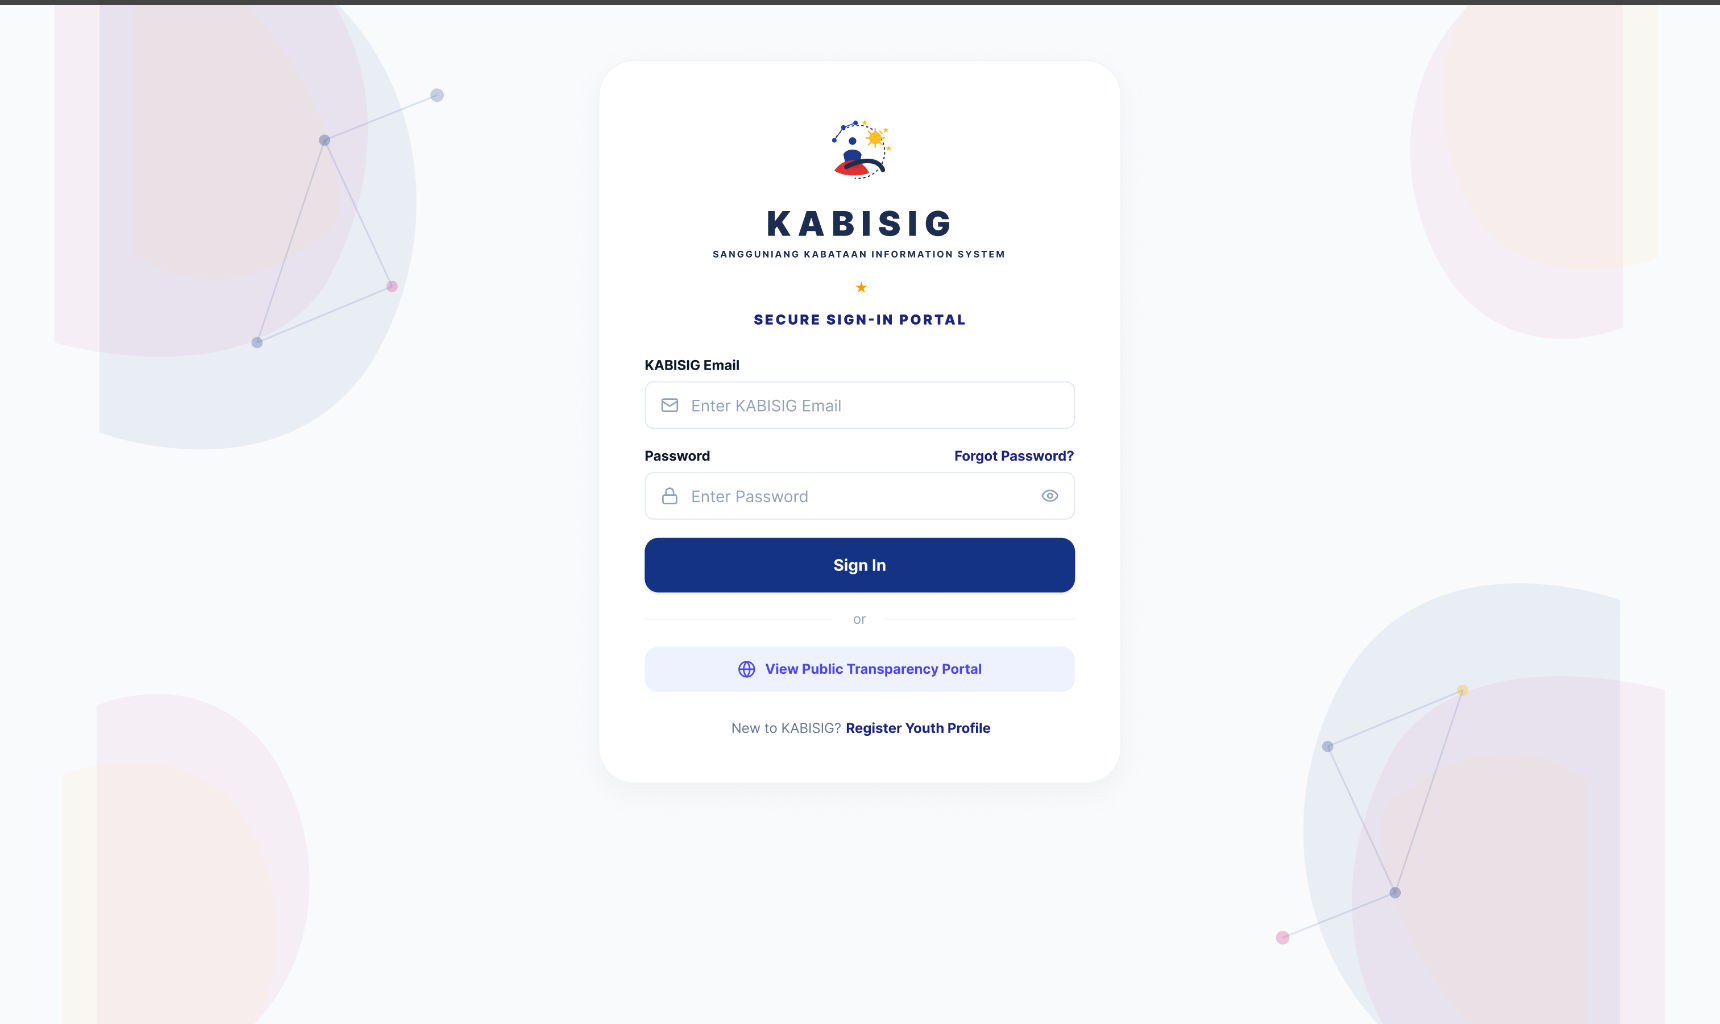
\includegraphics[width=0.45\textwidth]{figures/landing_page.png}
\caption{Public Transparency Portal and Landing Page (Sample Data)}
\label{fig:public_screens}
\end{figure}

\hspace*{\parindent} The authentication flow includes the Secure Sign-In Portal, Create Profile page, and Mandatory Password Change screen. Users are required to change temporary passwords upon first login, ensuring account security. The sign-in portal provides options for both registered users and public access to transparency data.\vspace{5mm}

\begin{figure}[H]
\centering
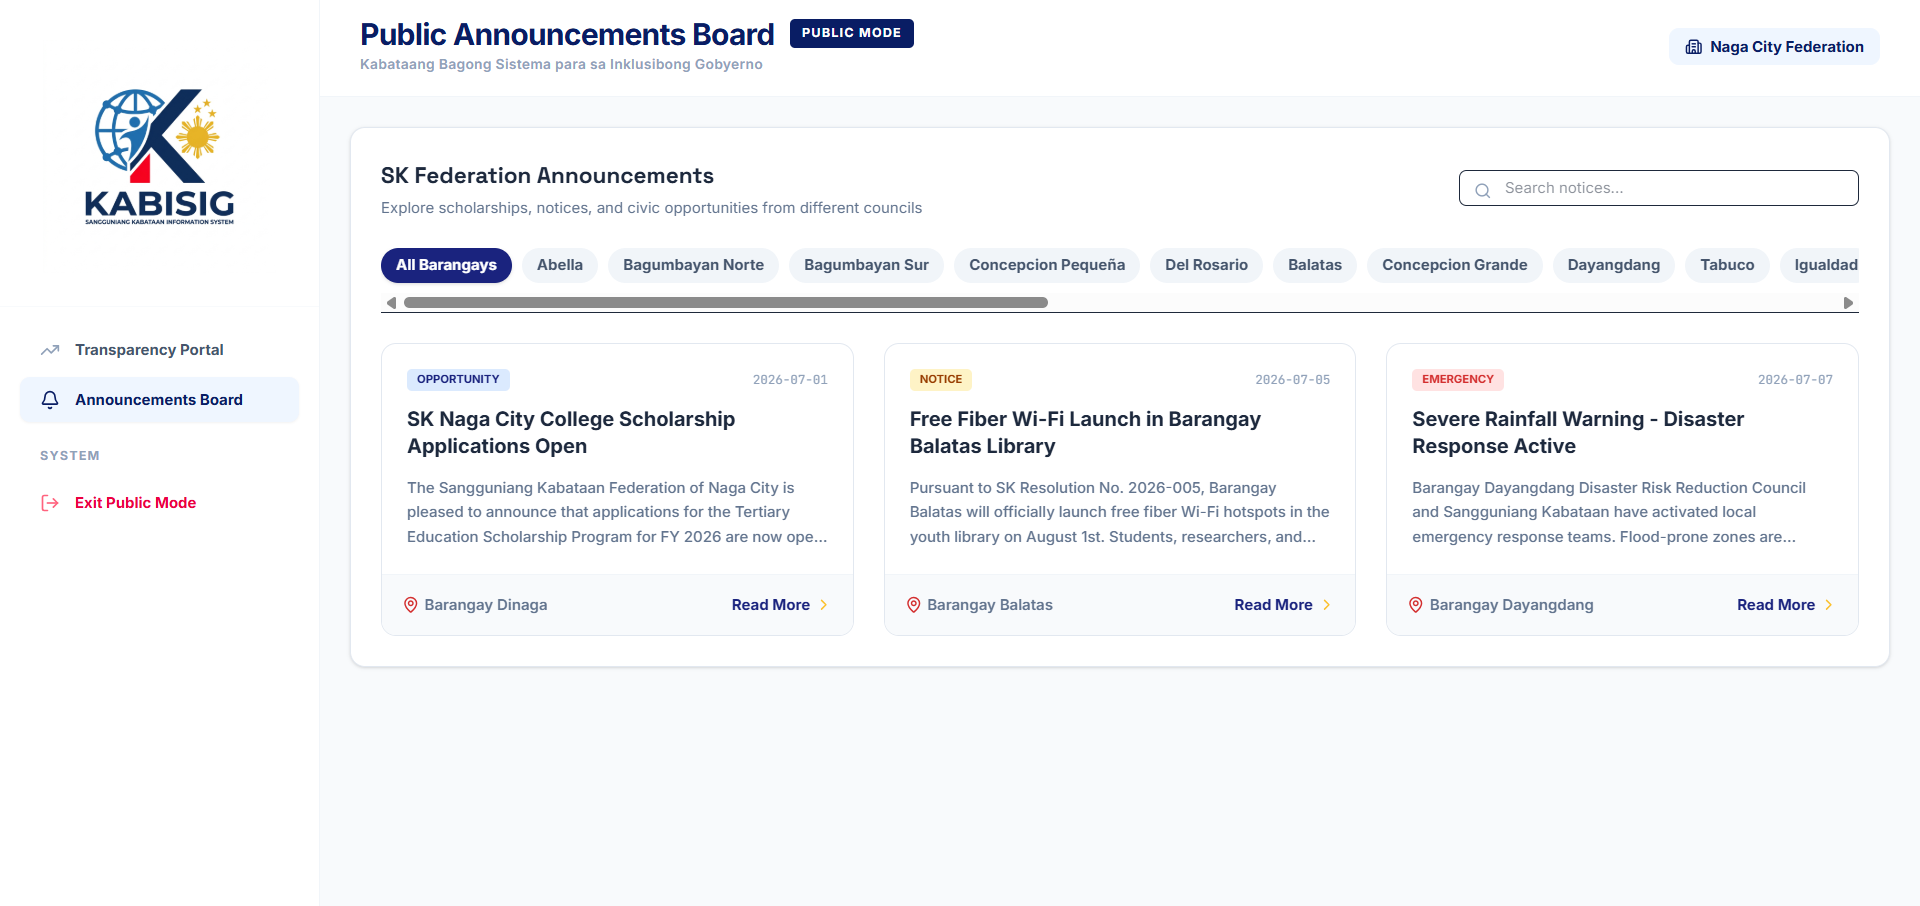
\includegraphics[width=0.30\textwidth]{figures/transparency_portal2.png}
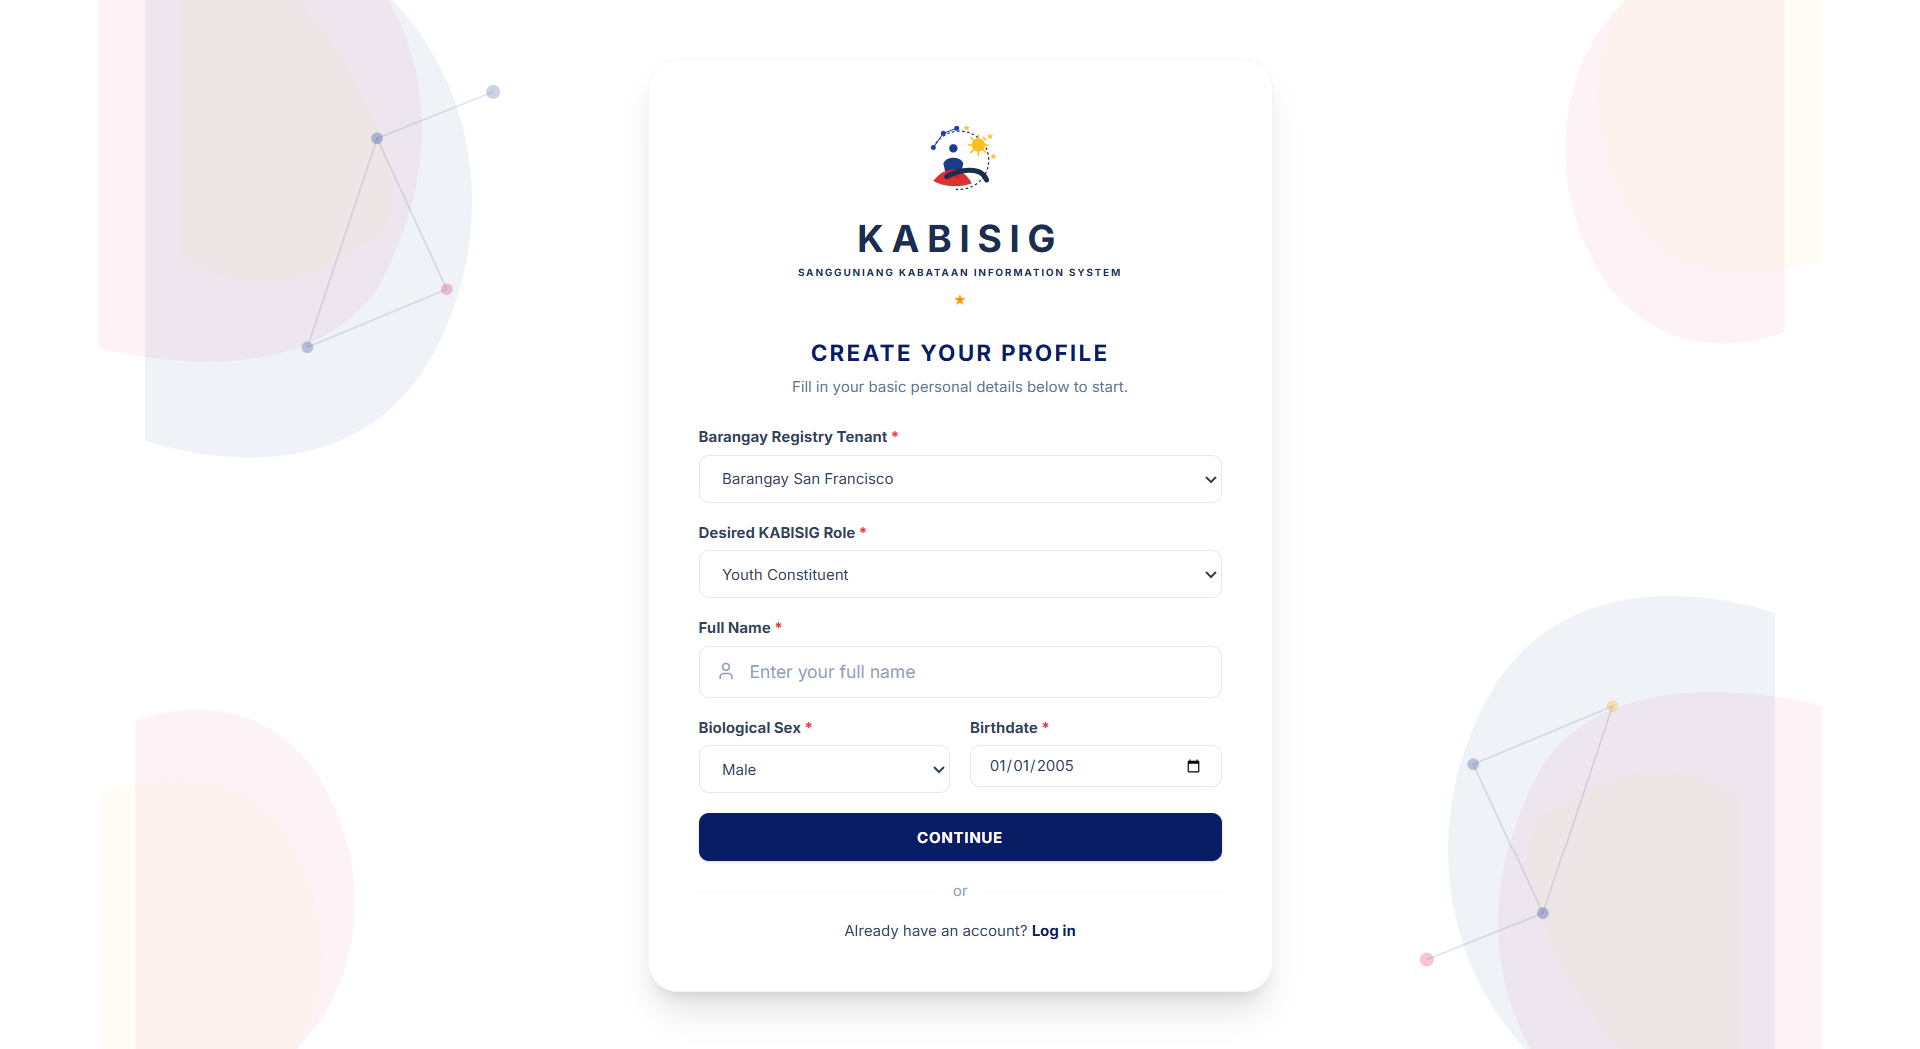
\includegraphics[width=0.30\textwidth]{figures/create_profile.png}
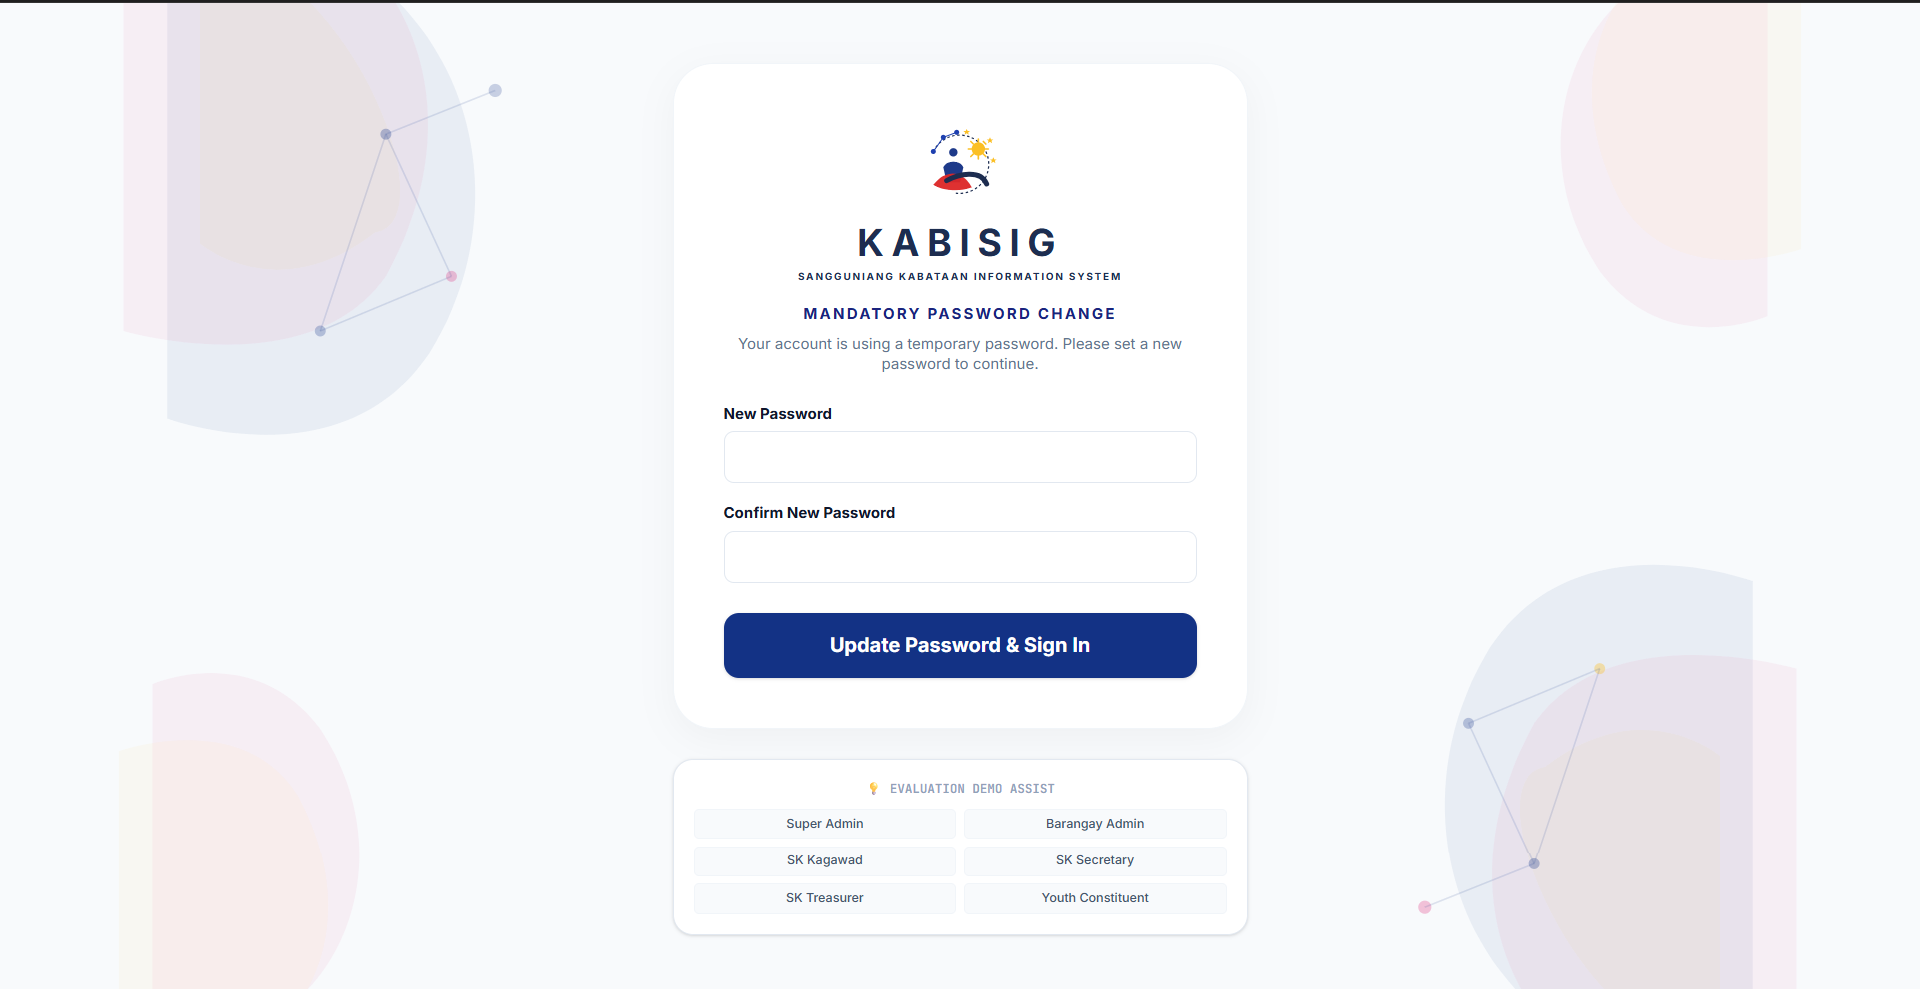
\includegraphics[width=0.30\textwidth]{figures/password_change.png}
\caption{Authentication Screens: Sign-In Portal, Create Profile, and Password Change (Sample Data)}
\label{fig:auth_screens}
\end{figure}

\subsubsection{Super Administrator Screens}

\hspace*{\parindent} The Super Administrator (SK Federation President) dashboard provides a comprehensive overview of all 27 barangays in Naga City. The Federation Dashboard displays key metrics including total barangays, total youth, active programs, and total budget. The welcome screen greets the SK Federation President with a personalized message and role badge, providing quick access to system-wide statistics and management tools.\vspace{5mm}

\begin{figure}[H]
\centering
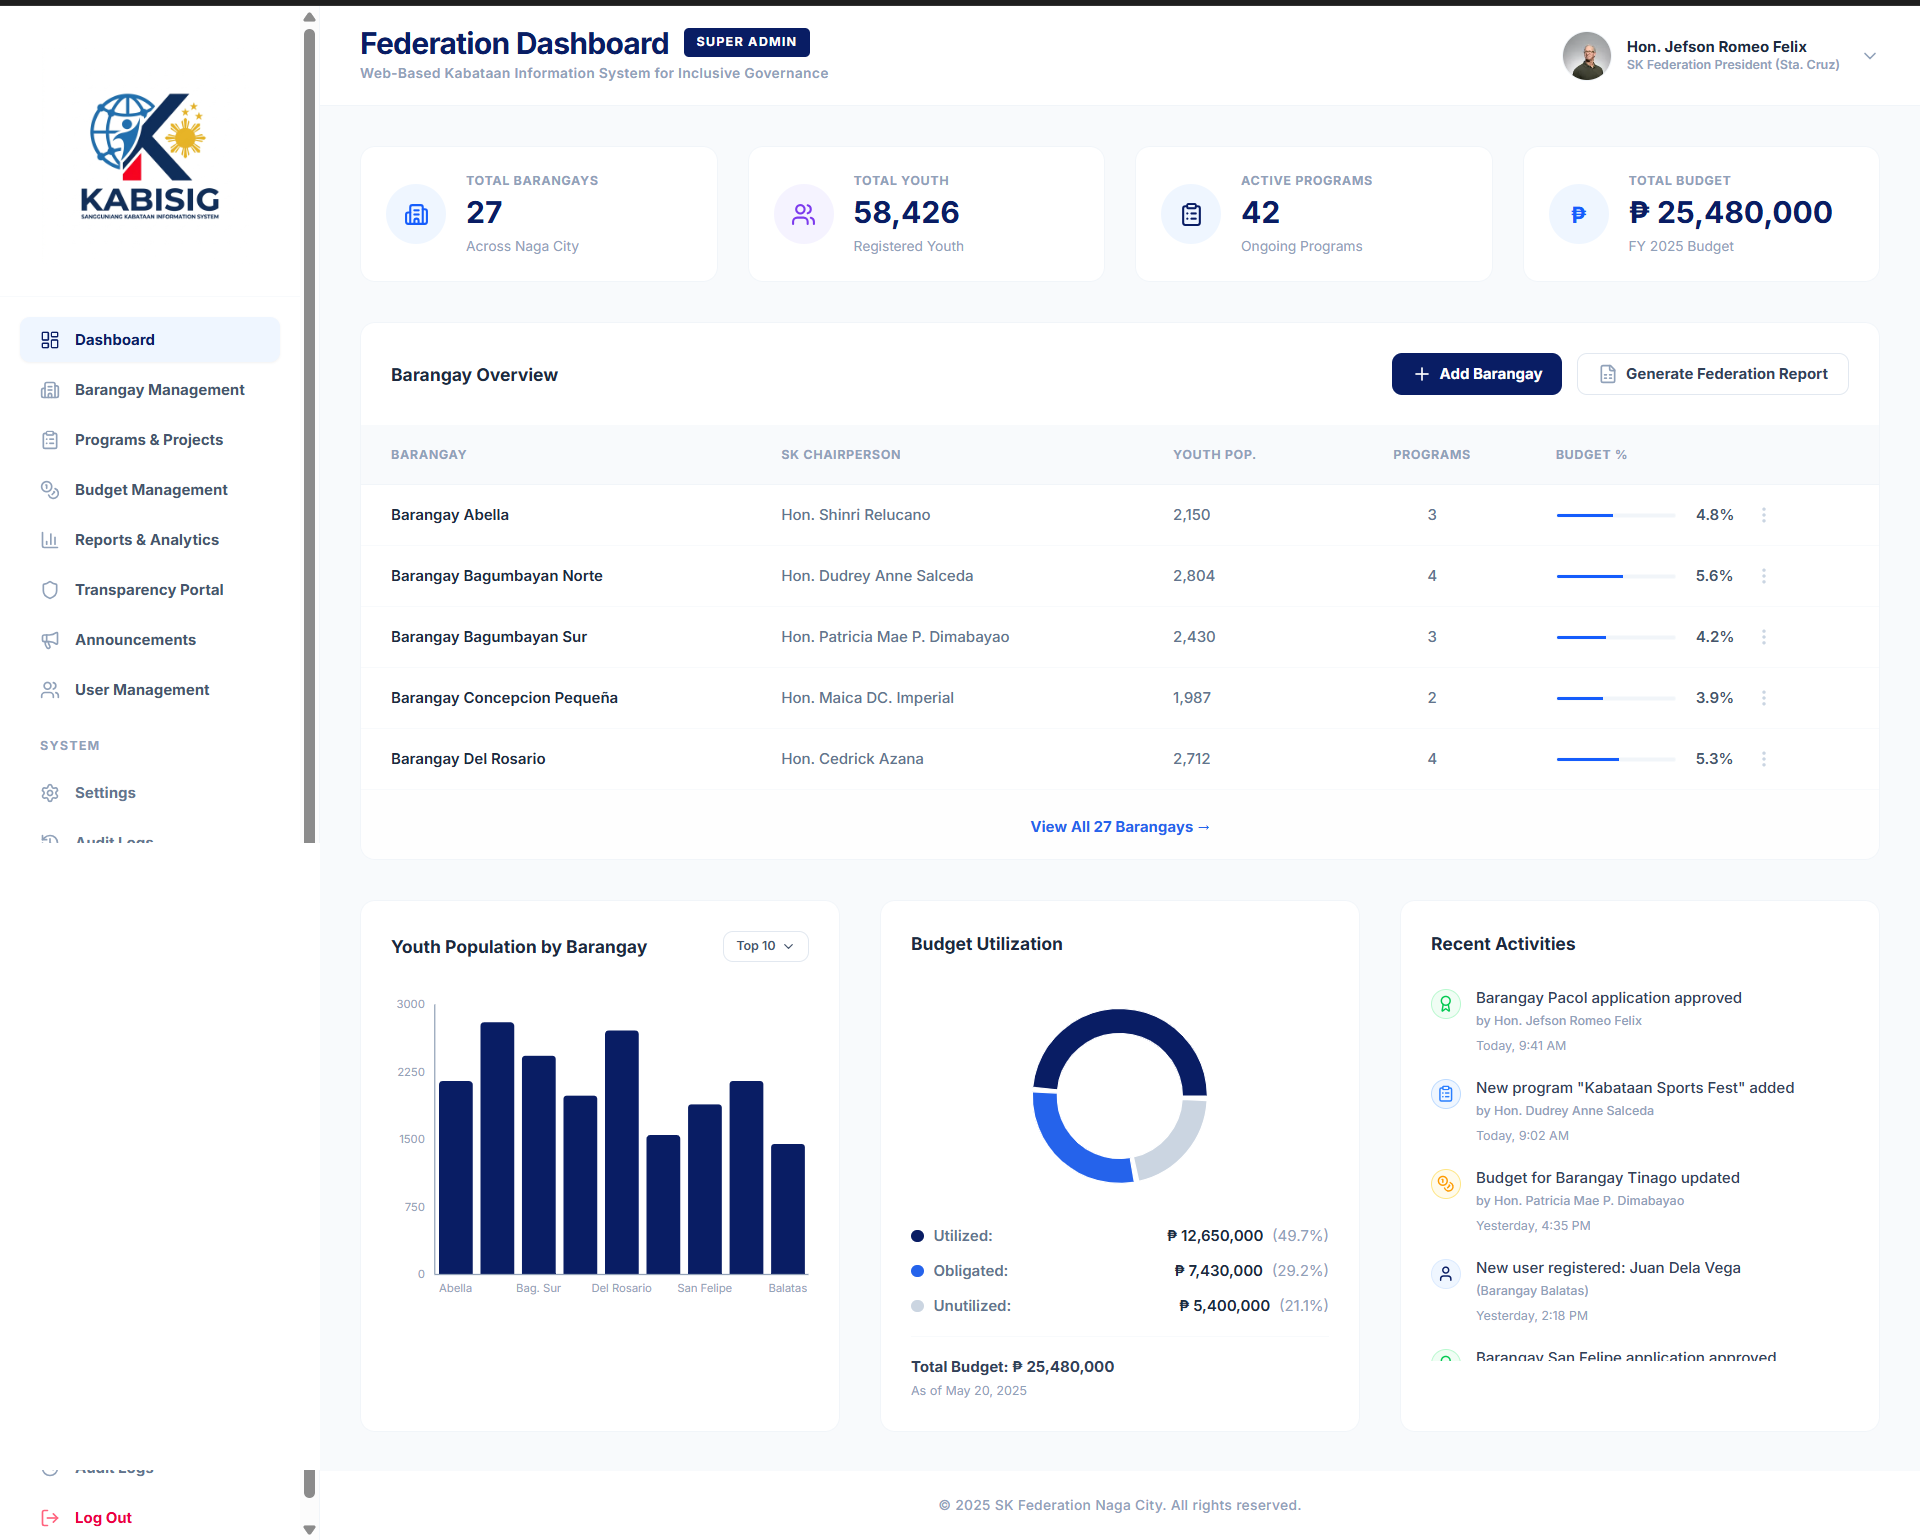
\includegraphics[width=0.45\textwidth]{figures/super_admin_dashboard.png}
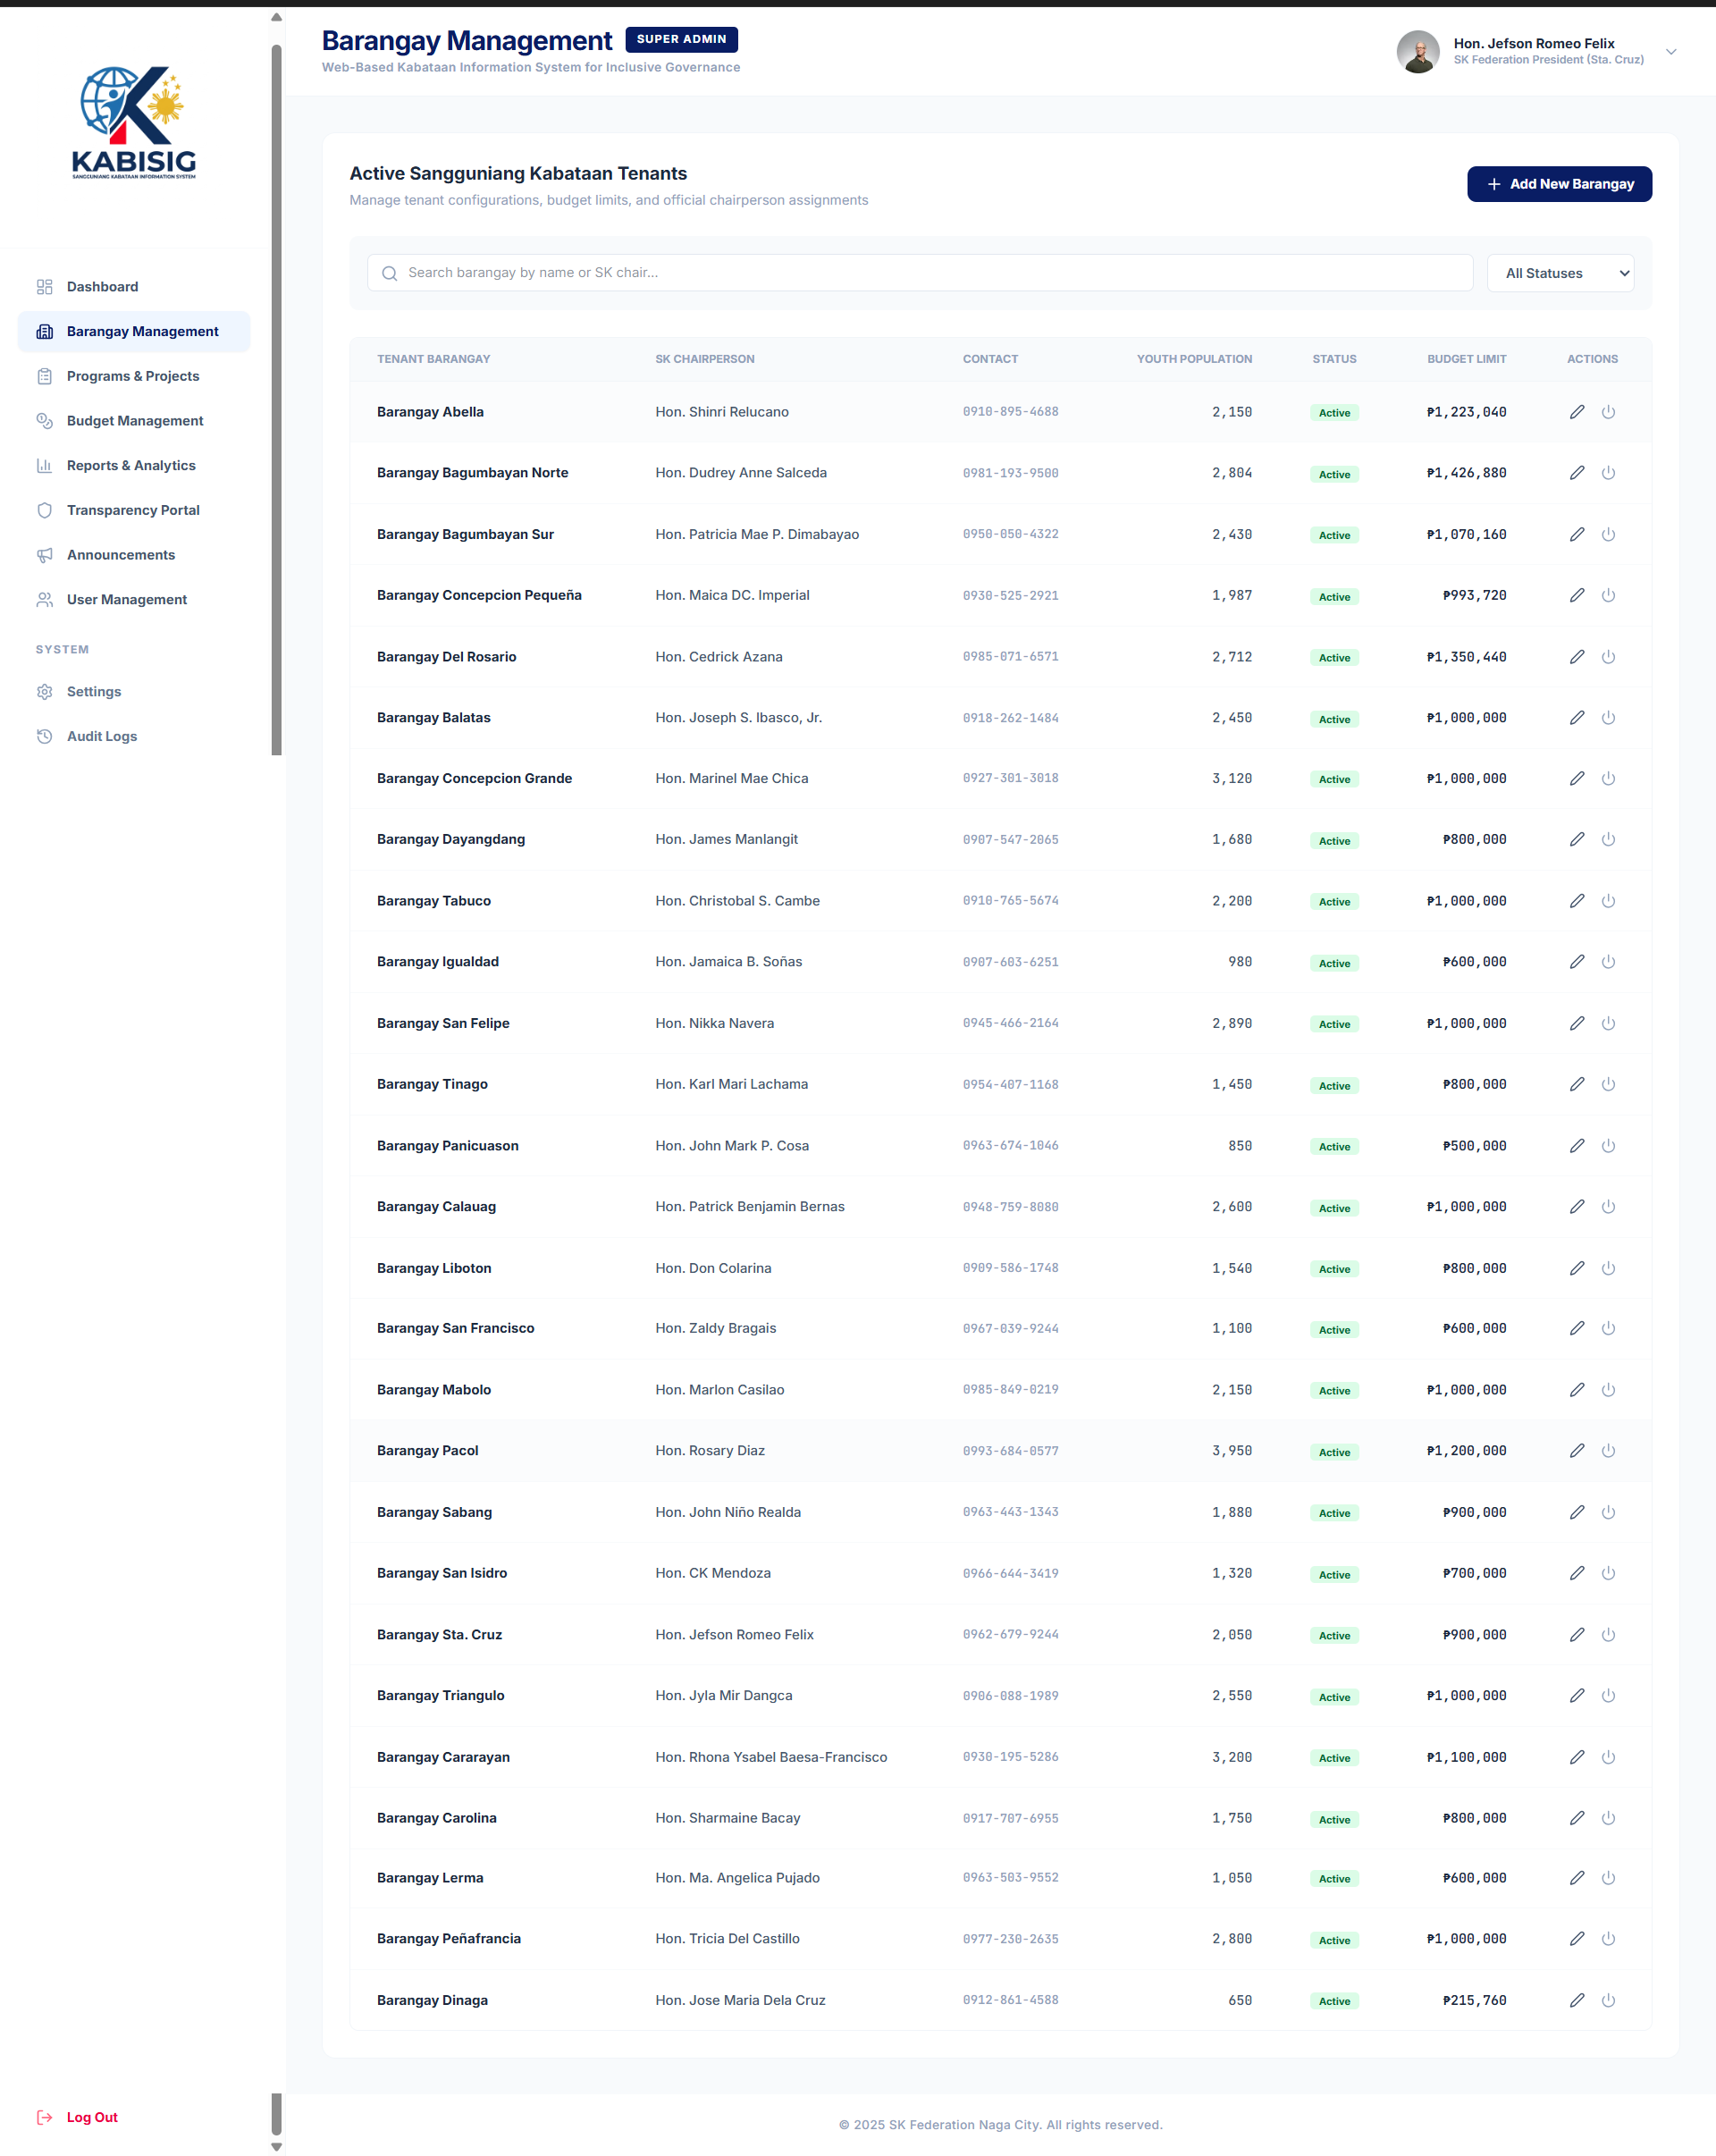
\includegraphics[width=0.45\textwidth]{figures/barangay_overview.png}
\caption{Super Administrator Federation Dashboard and Barangay Overview (Sample Data)}
\label{fig:super_admin}
\end{figure}

\hspace*{\parindent} The barangay overview lists each barangay with its SK Chairperson, youth population, program count, and budget utilization percentage. The dashboard also includes visual analytics such as Youth Population by Barangay charts and Budget Utilization distribution. Recent activities are logged for monitoring purposes, including barangay application approvals, program additions, and budget updates.\vspace{5mm}

\subsubsection{Barangay Administrator Screens}

\hspace*{\parindent} The Barangay Admin Dashboard provides SK Chairpersons with a focused view of their specific barangay's statistics and activities. Key metrics include youth population, active programs, total budget, and pending approvals. Quick action buttons provide access to Create Program, View Registrations, and Manage Documents functionalities.\vspace{5mm}

\begin{figure}[H]
\centering
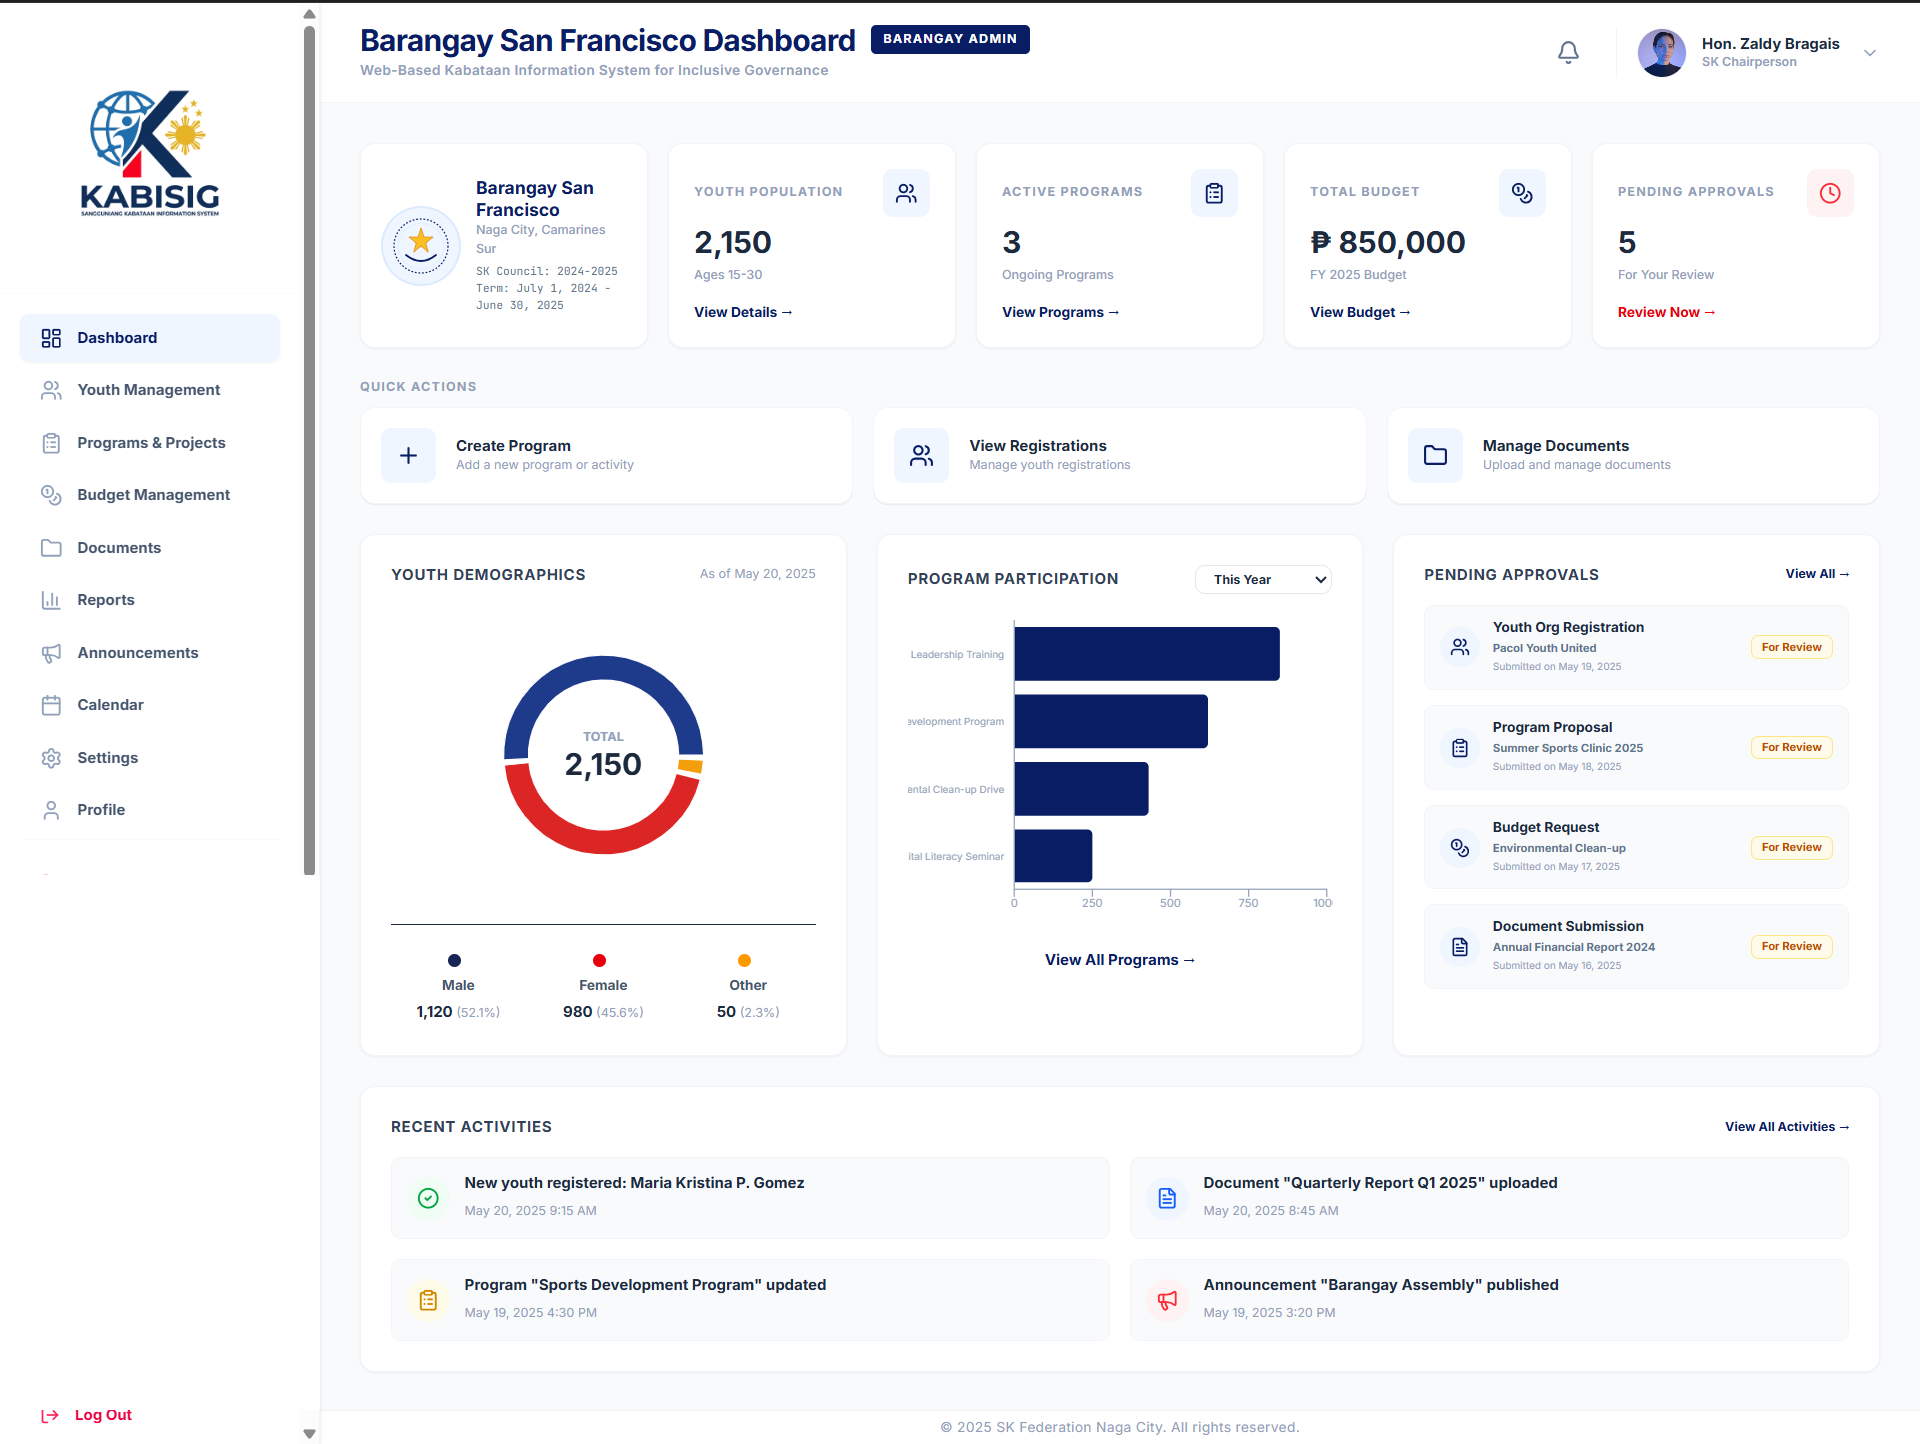
\includegraphics[width=0.45\textwidth]{figures/barangay_admin_dashboard.png}
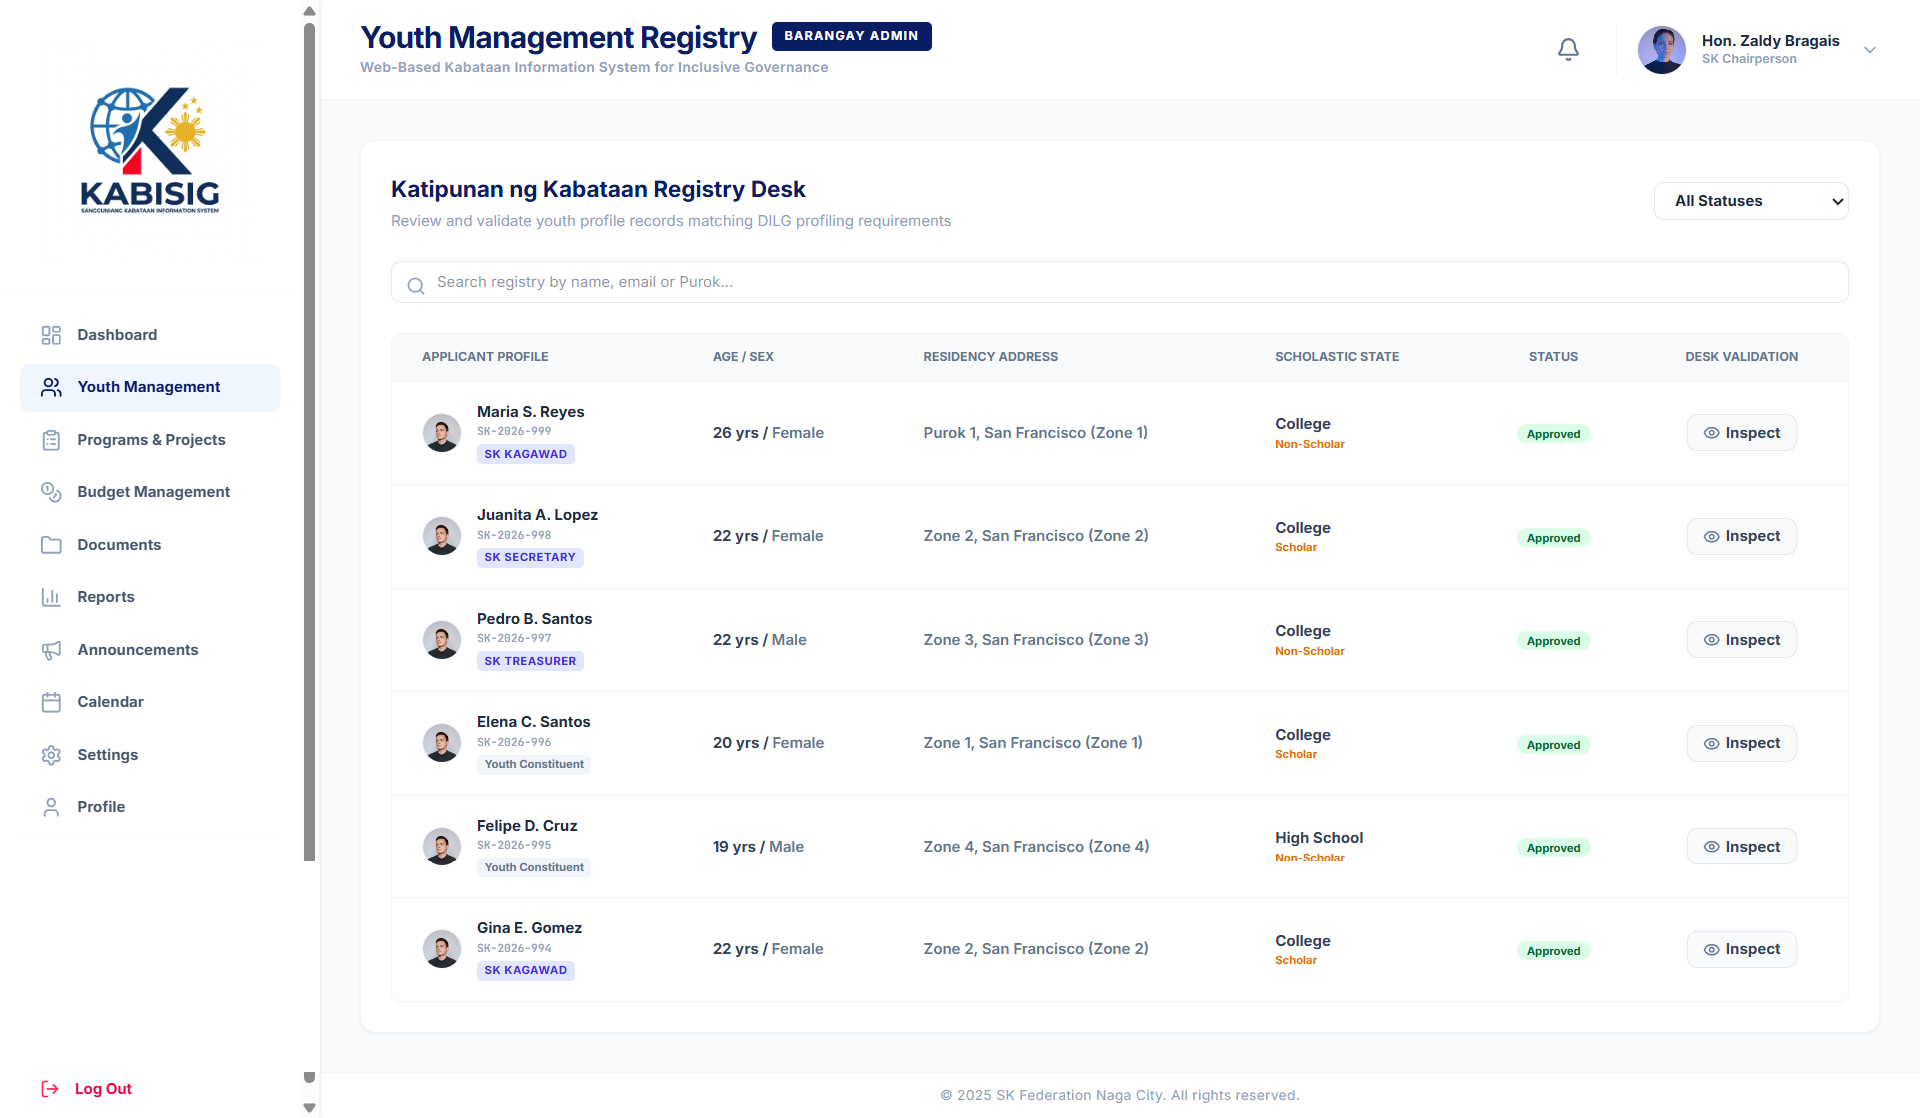
\includegraphics[width=0.45\textwidth]{figures/youth_management.png}
\caption{Barangay Admin Dashboard and Youth Management (Sample Data)}
\label{fig:barangay_admin}
\end{figure}

\hspace*{\parindent} The Youth Management module allows Barangay Admins to view and approve youth registrations, generate Digital Youth IDs, and manage beneficiary records. Pending registrations are displayed with approve/reject actions, ensuring only verified residents gain access to SK services.\vspace{5mm}

\hspace*{\parindent} The Facebook Page Synchronization module enables Barangay Admins to connect KABISIG with their official SK Facebook page. This feature ensures consistent public communication by automatically synchronizing announcements, program postings, and updates between KABISIG and Facebook. The Social Sync dashboard provides a comprehensive social announcements ledger with status tracking for all posts.\vspace{5mm}

\begin{figure}[H]
\centering
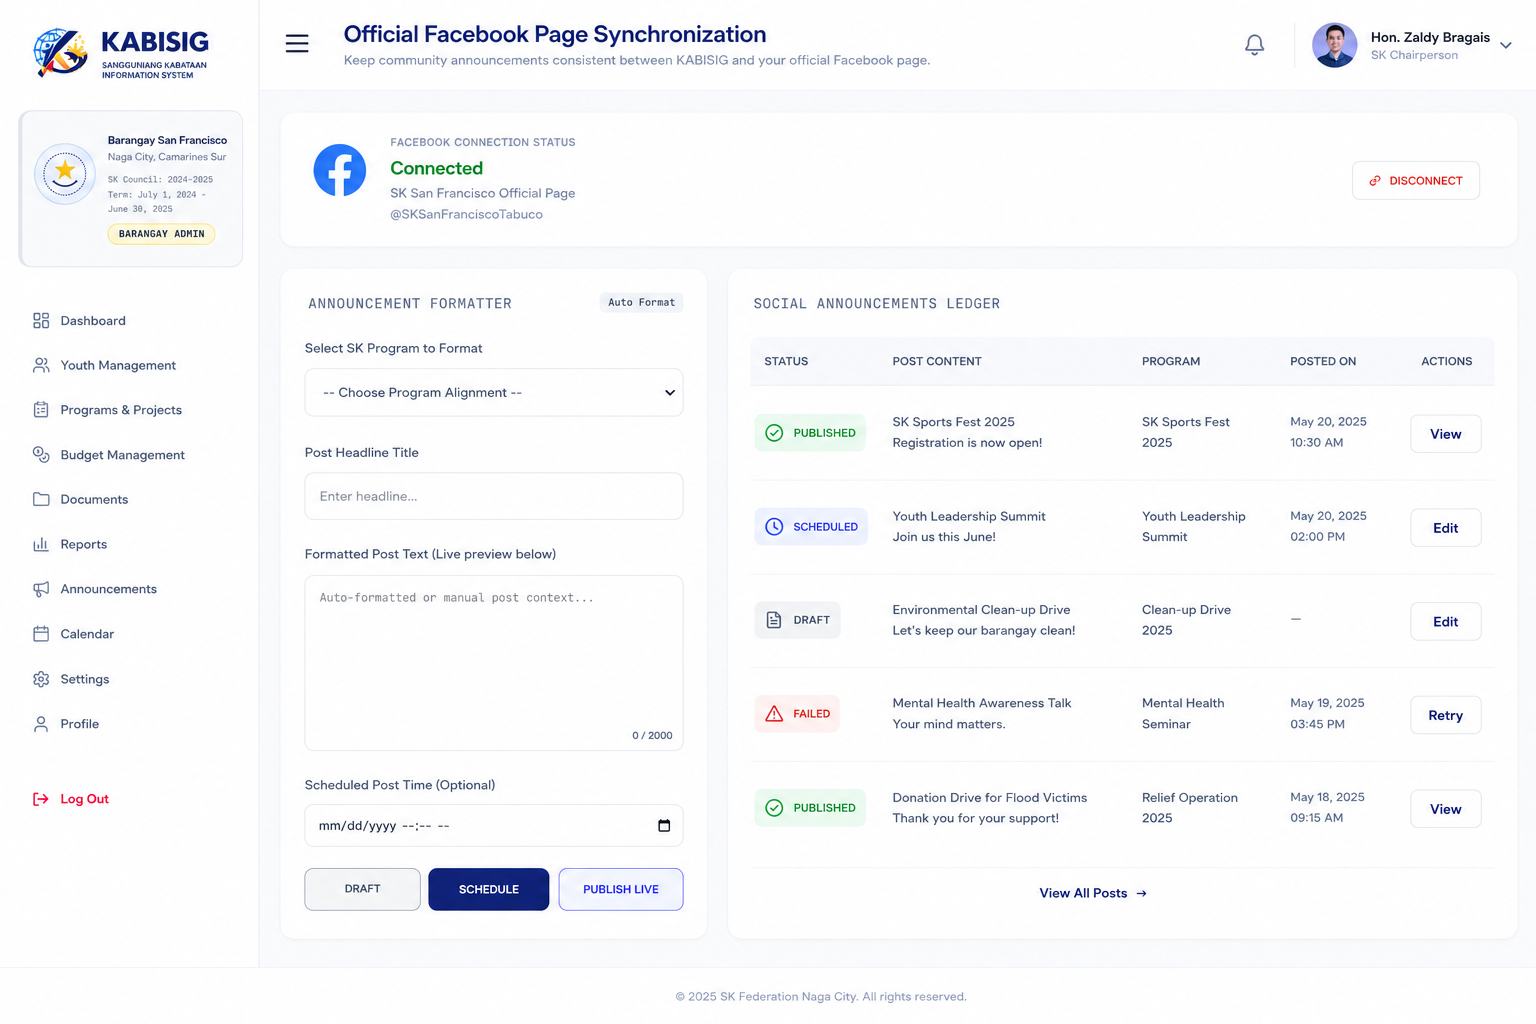
\includegraphics[width=0.45\textwidth]{figures/facebook_sync.png}
\caption{Barangay Admin Facebook Page Synchronization (Sample Data)}
\label{fig:facebook_sync}
\end{figure}

\hspace*{\parindent} The Social Sync interface includes the following key features:\vspace{3mm}

\begin{itemize}
    \item \textbf{Announcement Formatter:} Users can select SK programs to format, enter post headlines, and generate auto-formatted Facebook post content with live preview.
    \item \textbf{Post Status Tracking:} Each social media post is tracked with status badges (Published, Scheduled, Draft, Failed) for easy monitoring and management.
    \item \textbf{Social Announcements Ledger:} A comprehensive ledger displays all posts with their status, content, associated program, and posting date. Actions include View, Edit, and Retry for failed posts.
    \item \textbf{Scheduled Posting:} Users can schedule posts for future publication with configurable date and time.
    \item \textbf{Post Statistics:} Summary cards show the count of Scheduled, Draft, and Published posts for quick overview.
\end{itemize}

\vspace{5mm}

\subsubsection{SK Kagawad Screens}

\hspace*{\parindent} The SK Kagawad workspace includes the Attendance Tracking module with QR scanner functionality. The scanner uses the device's camera via WebRTC and the Web Barcode Detection API, allowing officials to scan youth QR codes for attendance marking. Manual entry mode is also available as a backup option.\vspace{5mm}

\begin{figure}[H]
\centering
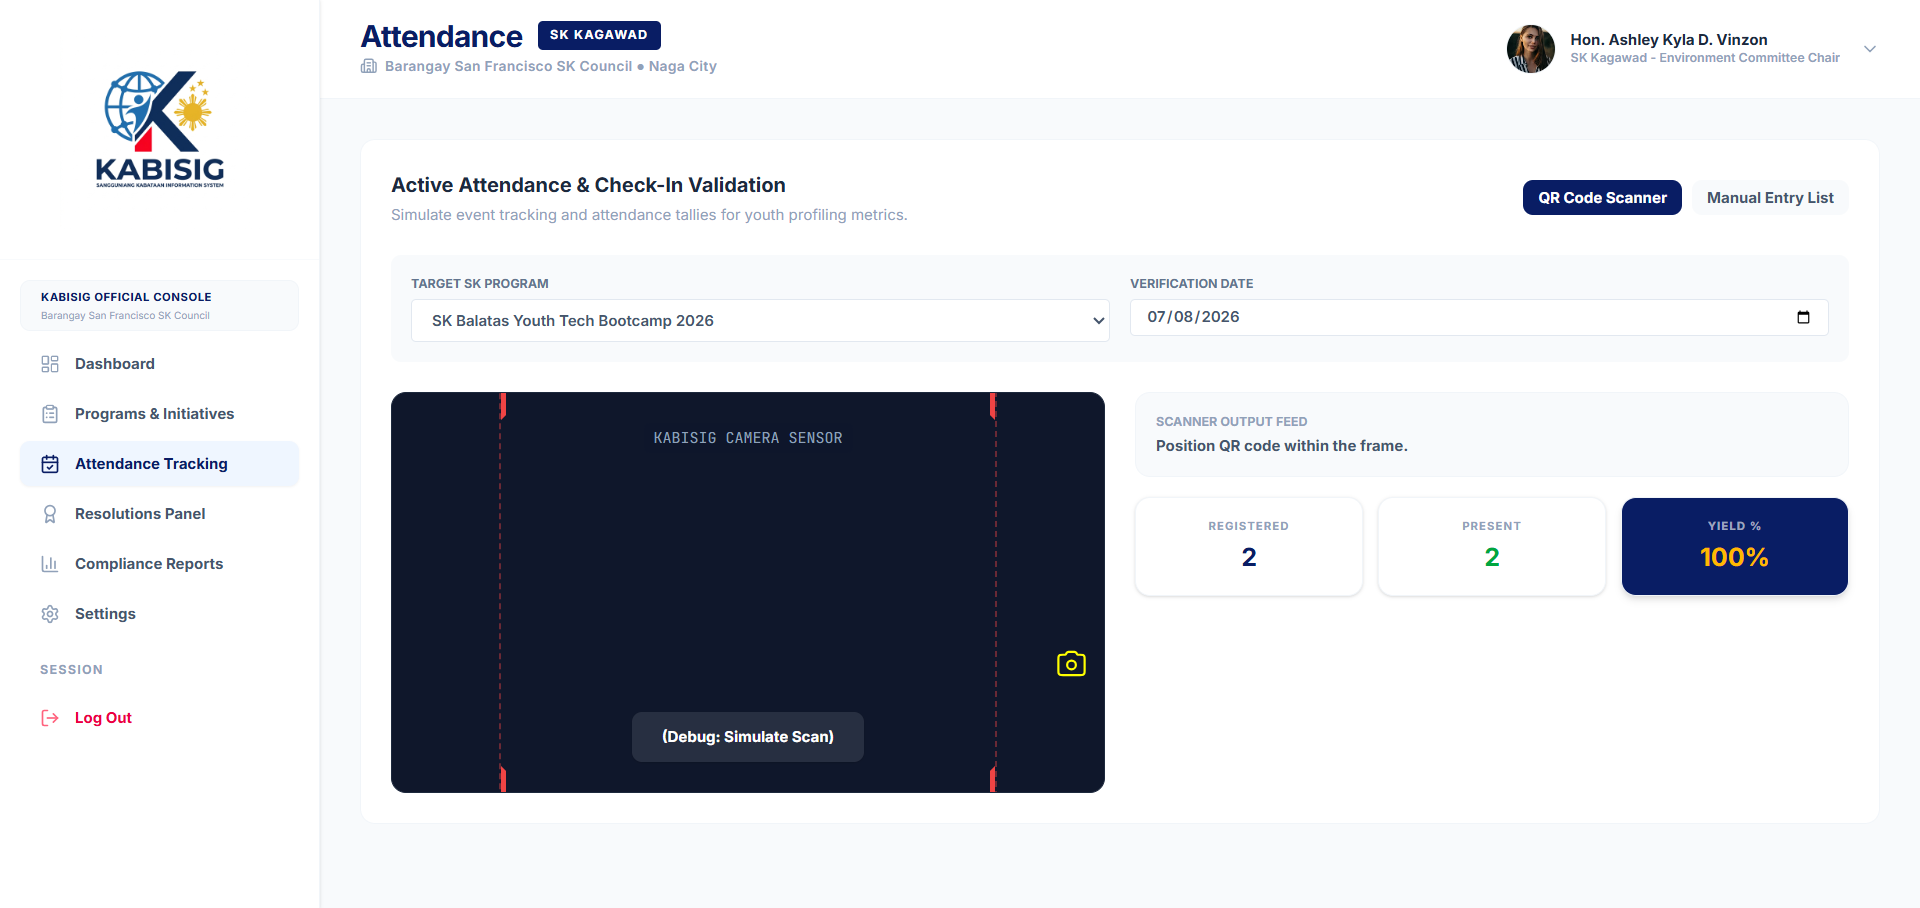
\includegraphics[width=0.45\textwidth]{figures/kagawad_attendance.png}
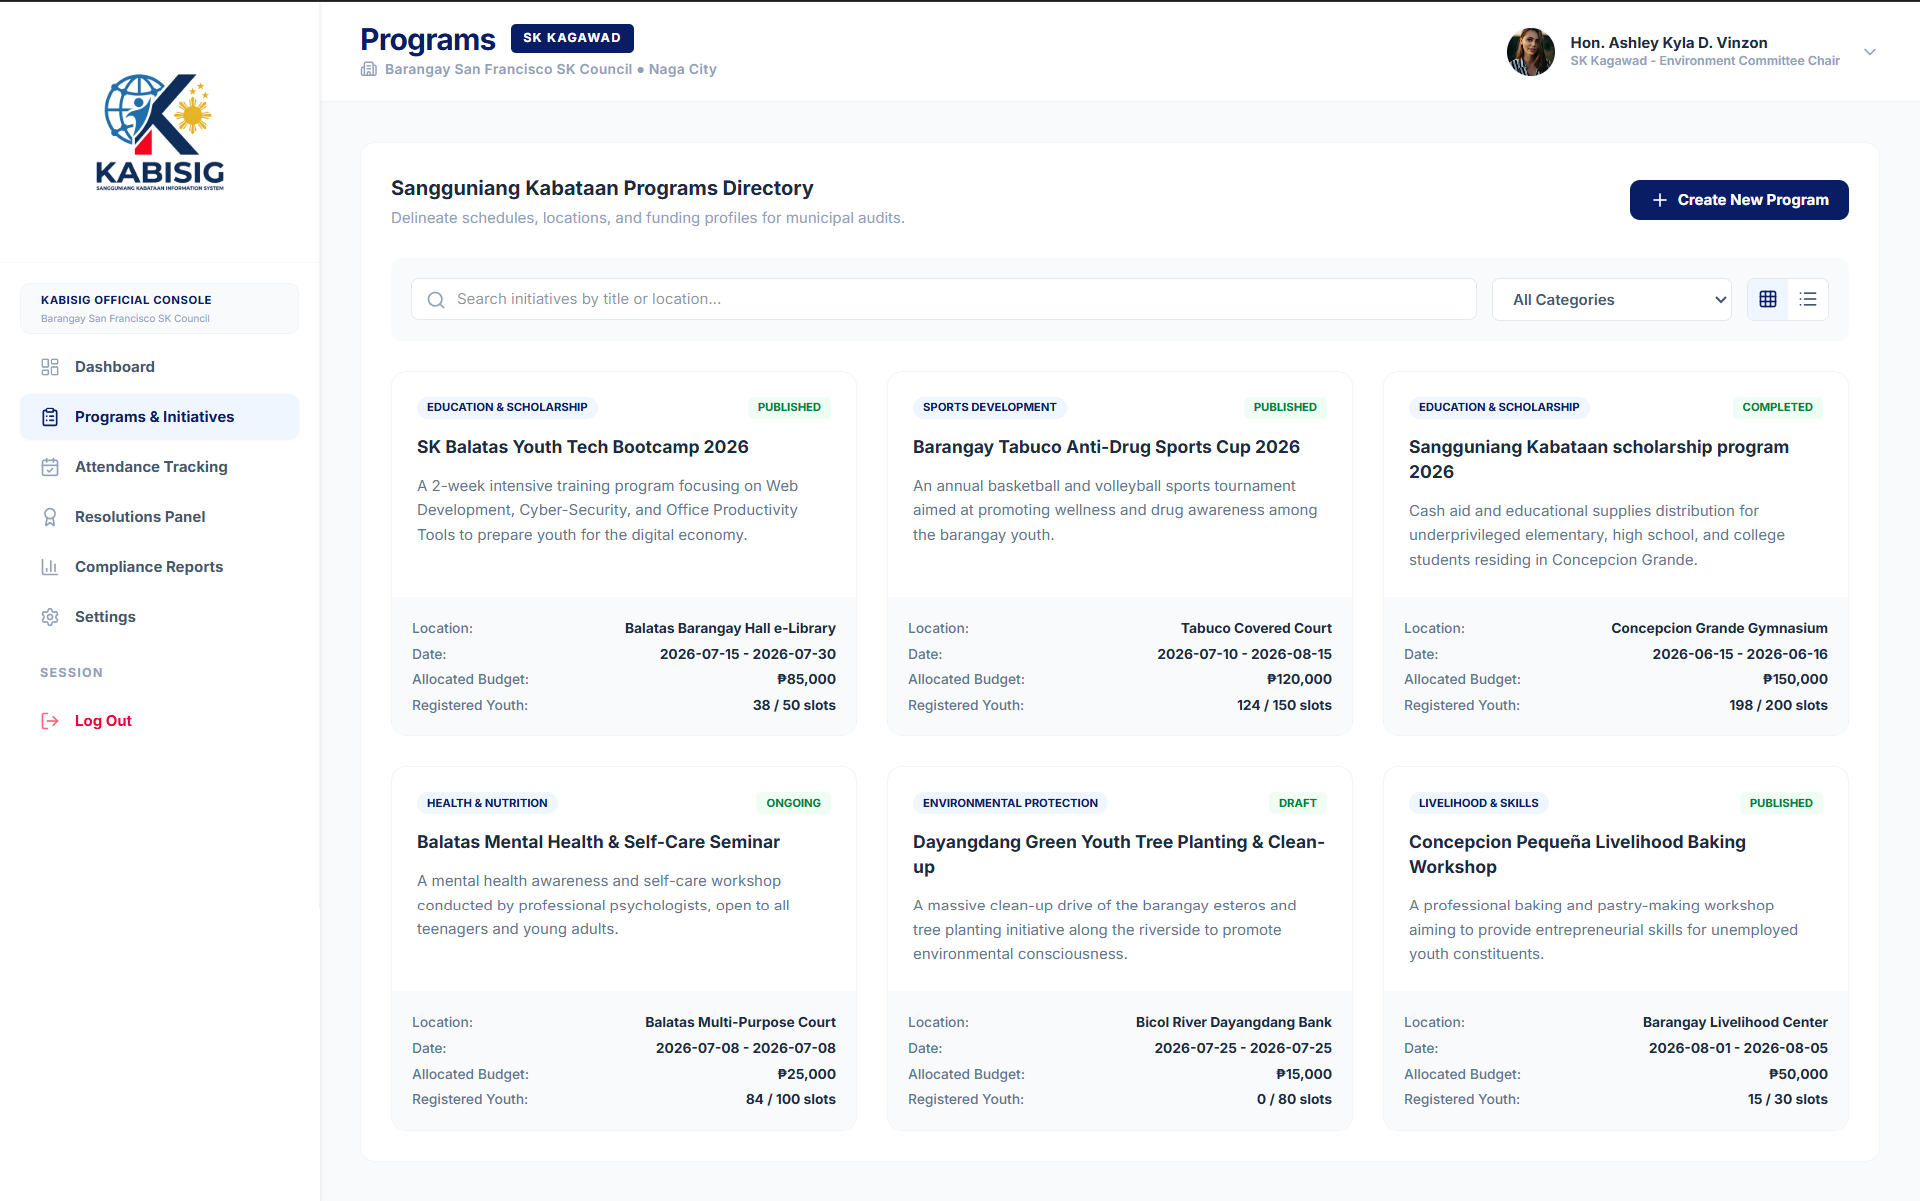
\includegraphics[width=0.45\textwidth]{figures/program_management.png}
\caption{SK Kagawad Attendance Tracking and Program Management (Sample Data)}
\label{fig:kagawad}
\end{figure}

\hspace*{\parindent} The Program Management screen displays program cards with key information including title, date, status, budget, and registrations. SK Kagawad can create, edit, and manage programs, with calendar view and list view options for flexible program tracking.\vspace{5mm}

\subsubsection{SK Secretary Screens}

\hspace*{\parindent} The SK Secretary Document Repository provides centralized document management for governance documents. Users can upload documents, categorize them by type (Resolutions, Vouchers, Reports, Budget), and track document status (Approved, Pending, Draft). The search and filter functionality enables efficient document retrieval.\vspace{5mm}

\begin{figure}[H]
\centering
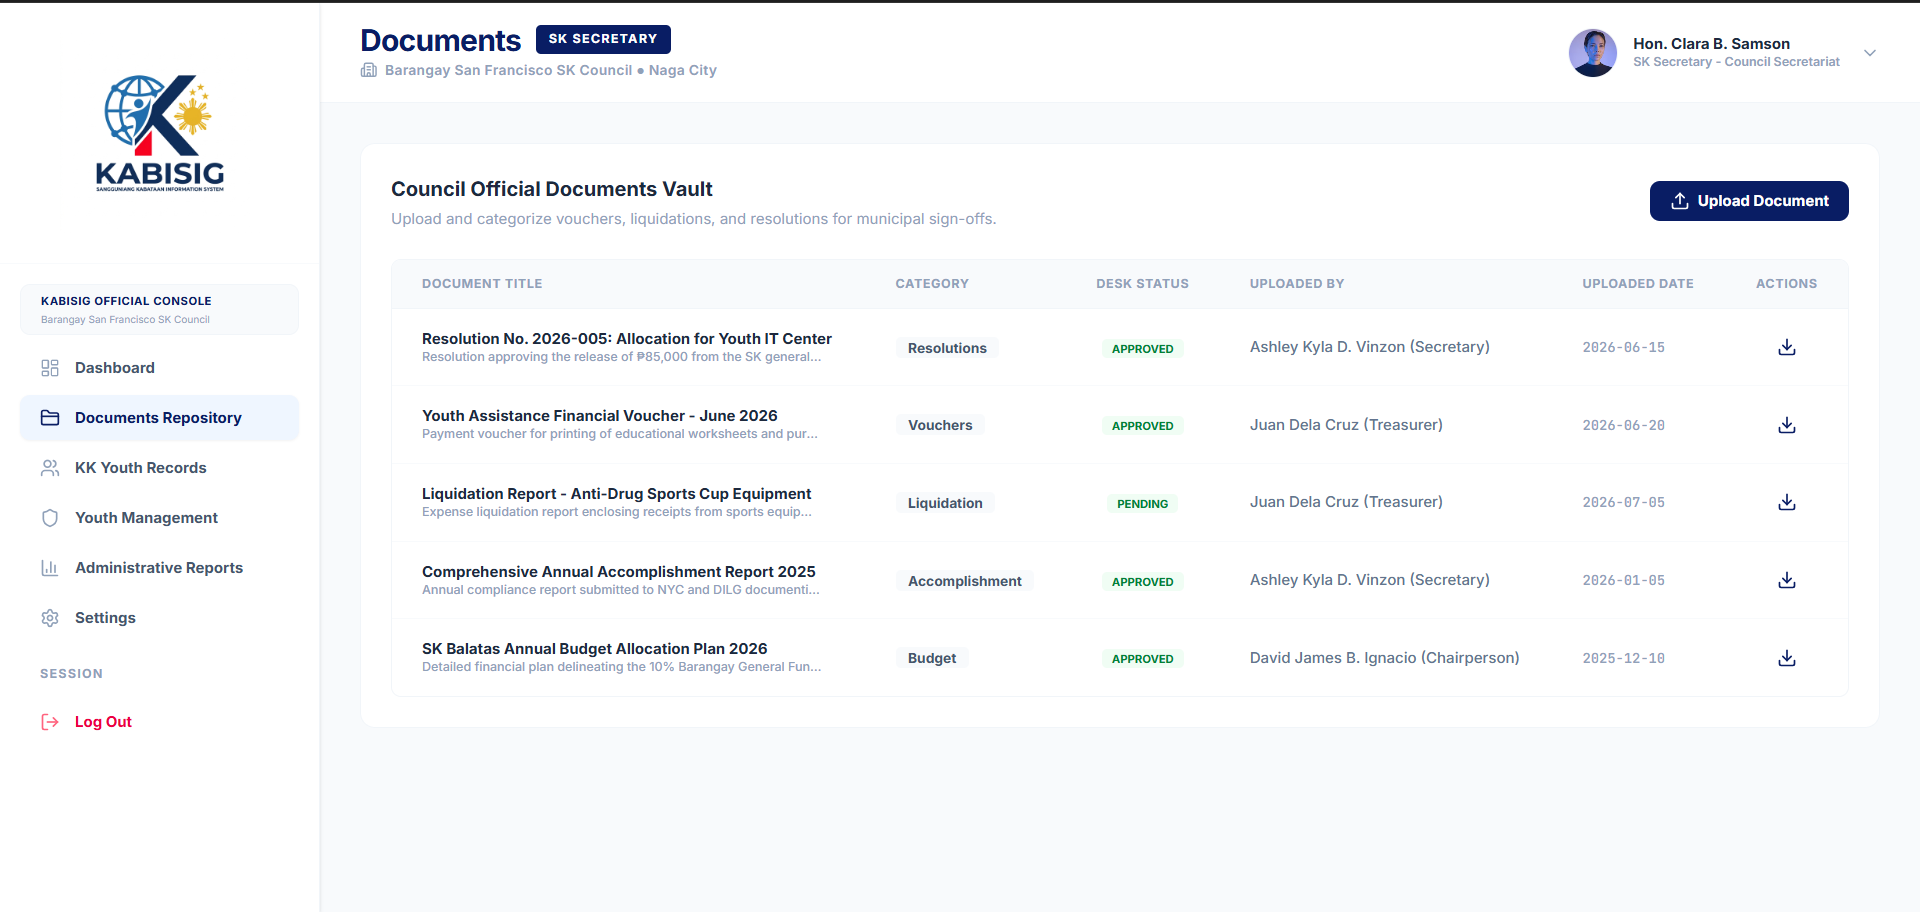
\includegraphics[width=0.45\textwidth]{figures/document_repository.png}
\caption{SK Secretary Document Repository (Sample Data)}
\label{fig:secretary}
\end{figure}

\hspace*{\parindent} Each document card displays the title, description, status badge, and date. Status badges use color coding: Approved (Green), Pending (Yellow), and Draft (Gray). Document actions include View, Download, Edit, and Route for Approval.\vspace{5mm}

\subsubsection{SK Treasurer Screens}

\hspace*{\parindent} The SK Treasurer Inventory Registry tracks SK council properties and assets. The interface displays property items with category group, quantity, condition, and location information. Users can register new assets and search the inventory.\vspace{5mm}

\begin{figure}[H]
\centering
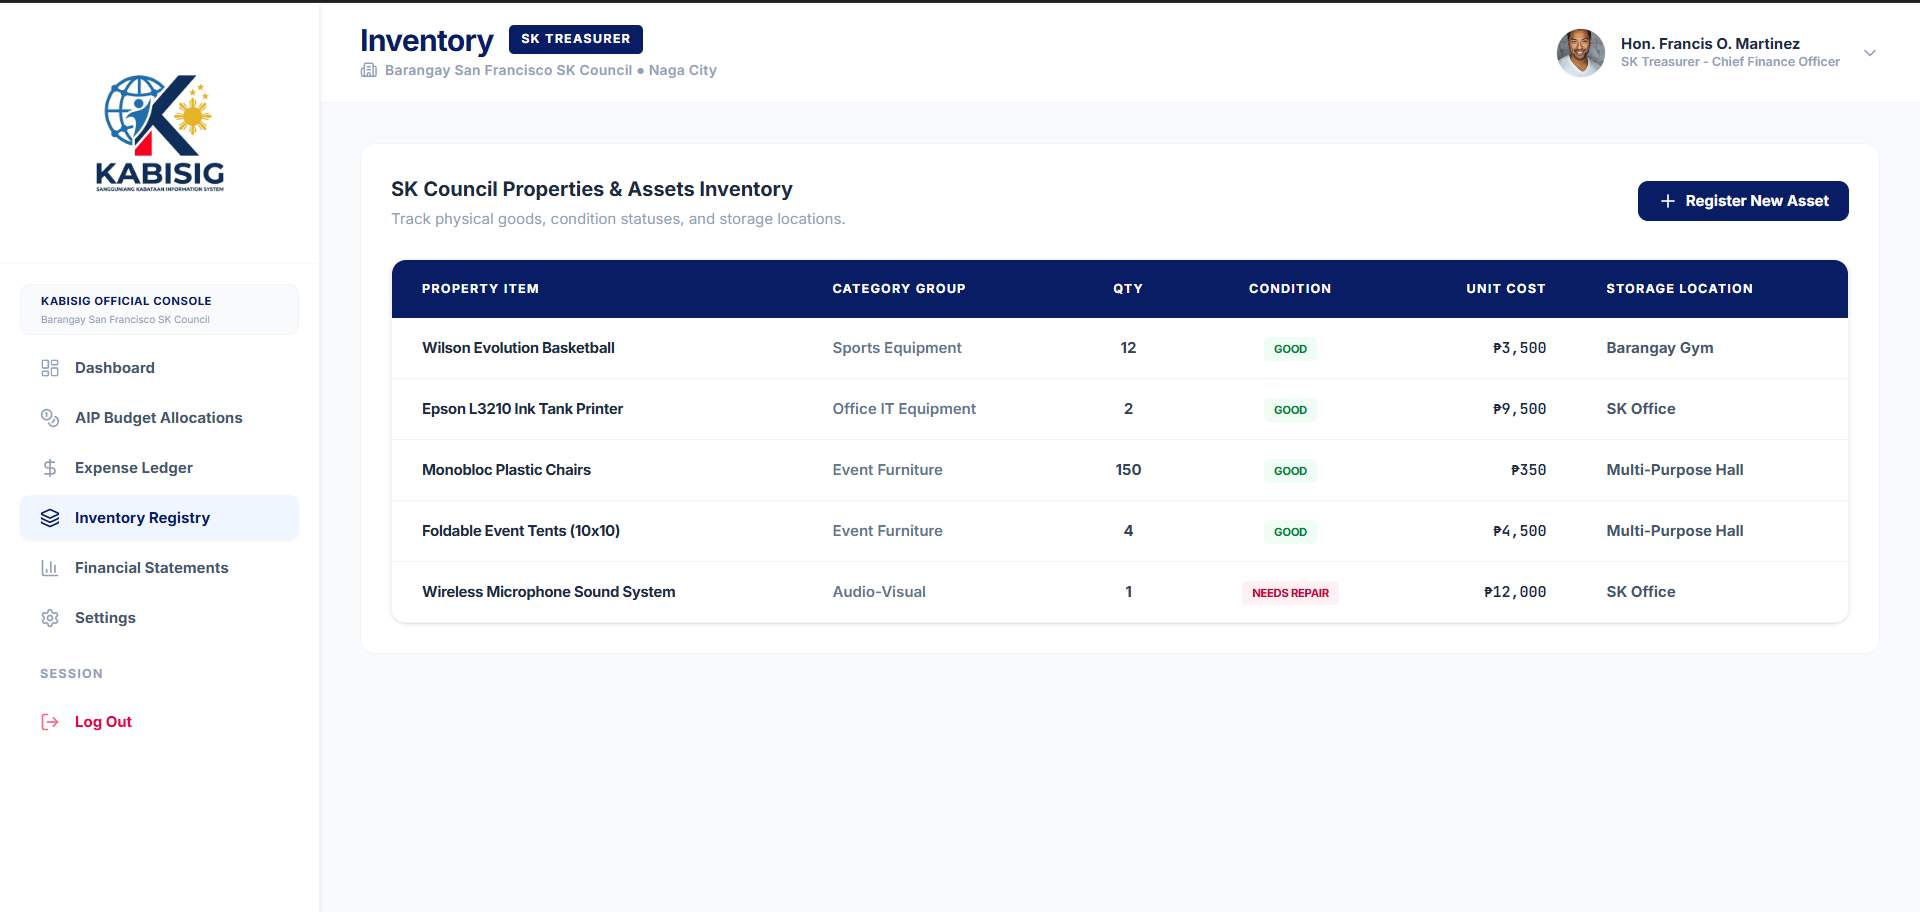
\includegraphics[width=0.45\textwidth]{figures/treasurer_inventory.png}
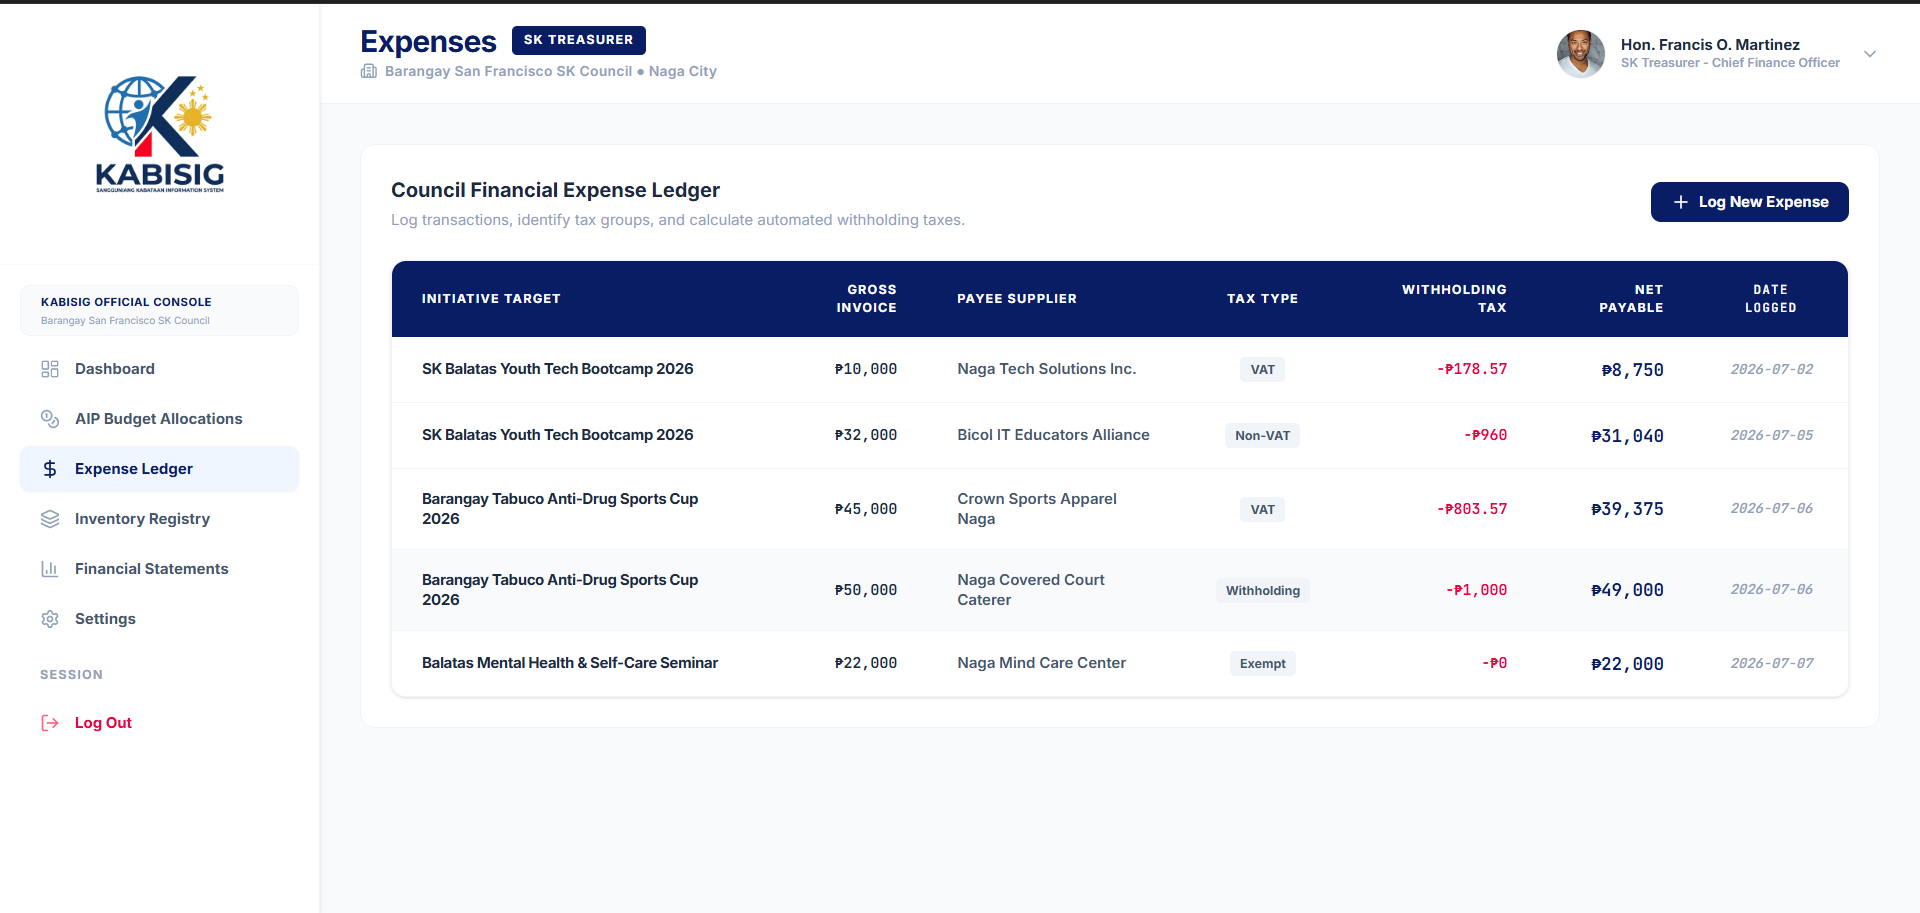
\includegraphics[width=0.45\textwidth]{figures/Expense_management.png}
\caption{SK Treasurer Inventory Registry and Budget Management (Sample Data)}
\label{fig:treasurer}
\end{figure}

\hspace*{\parindent} The Budget Management screen provides financial oversight with automated VAT/Non-VAT computation. Expense items display initiative description, gross amount, tax class, net disbursement, and status. The system automatically generates budget utilization reports and alerts for overspending.\vspace{5mm}

\subsubsection{Youth Constituent Screens}

\hspace*{\parindent} The Youth Dashboard provides a personalized homepage for youth constituents, displaying their Digital Youth ID, key statistics (barangay youth population, ongoing programs, participation count, active polls), and upcoming programs. The Digital Youth ID includes serial number, address, and verification status.\vspace{5mm}

\begin{figure}[H]
\centering
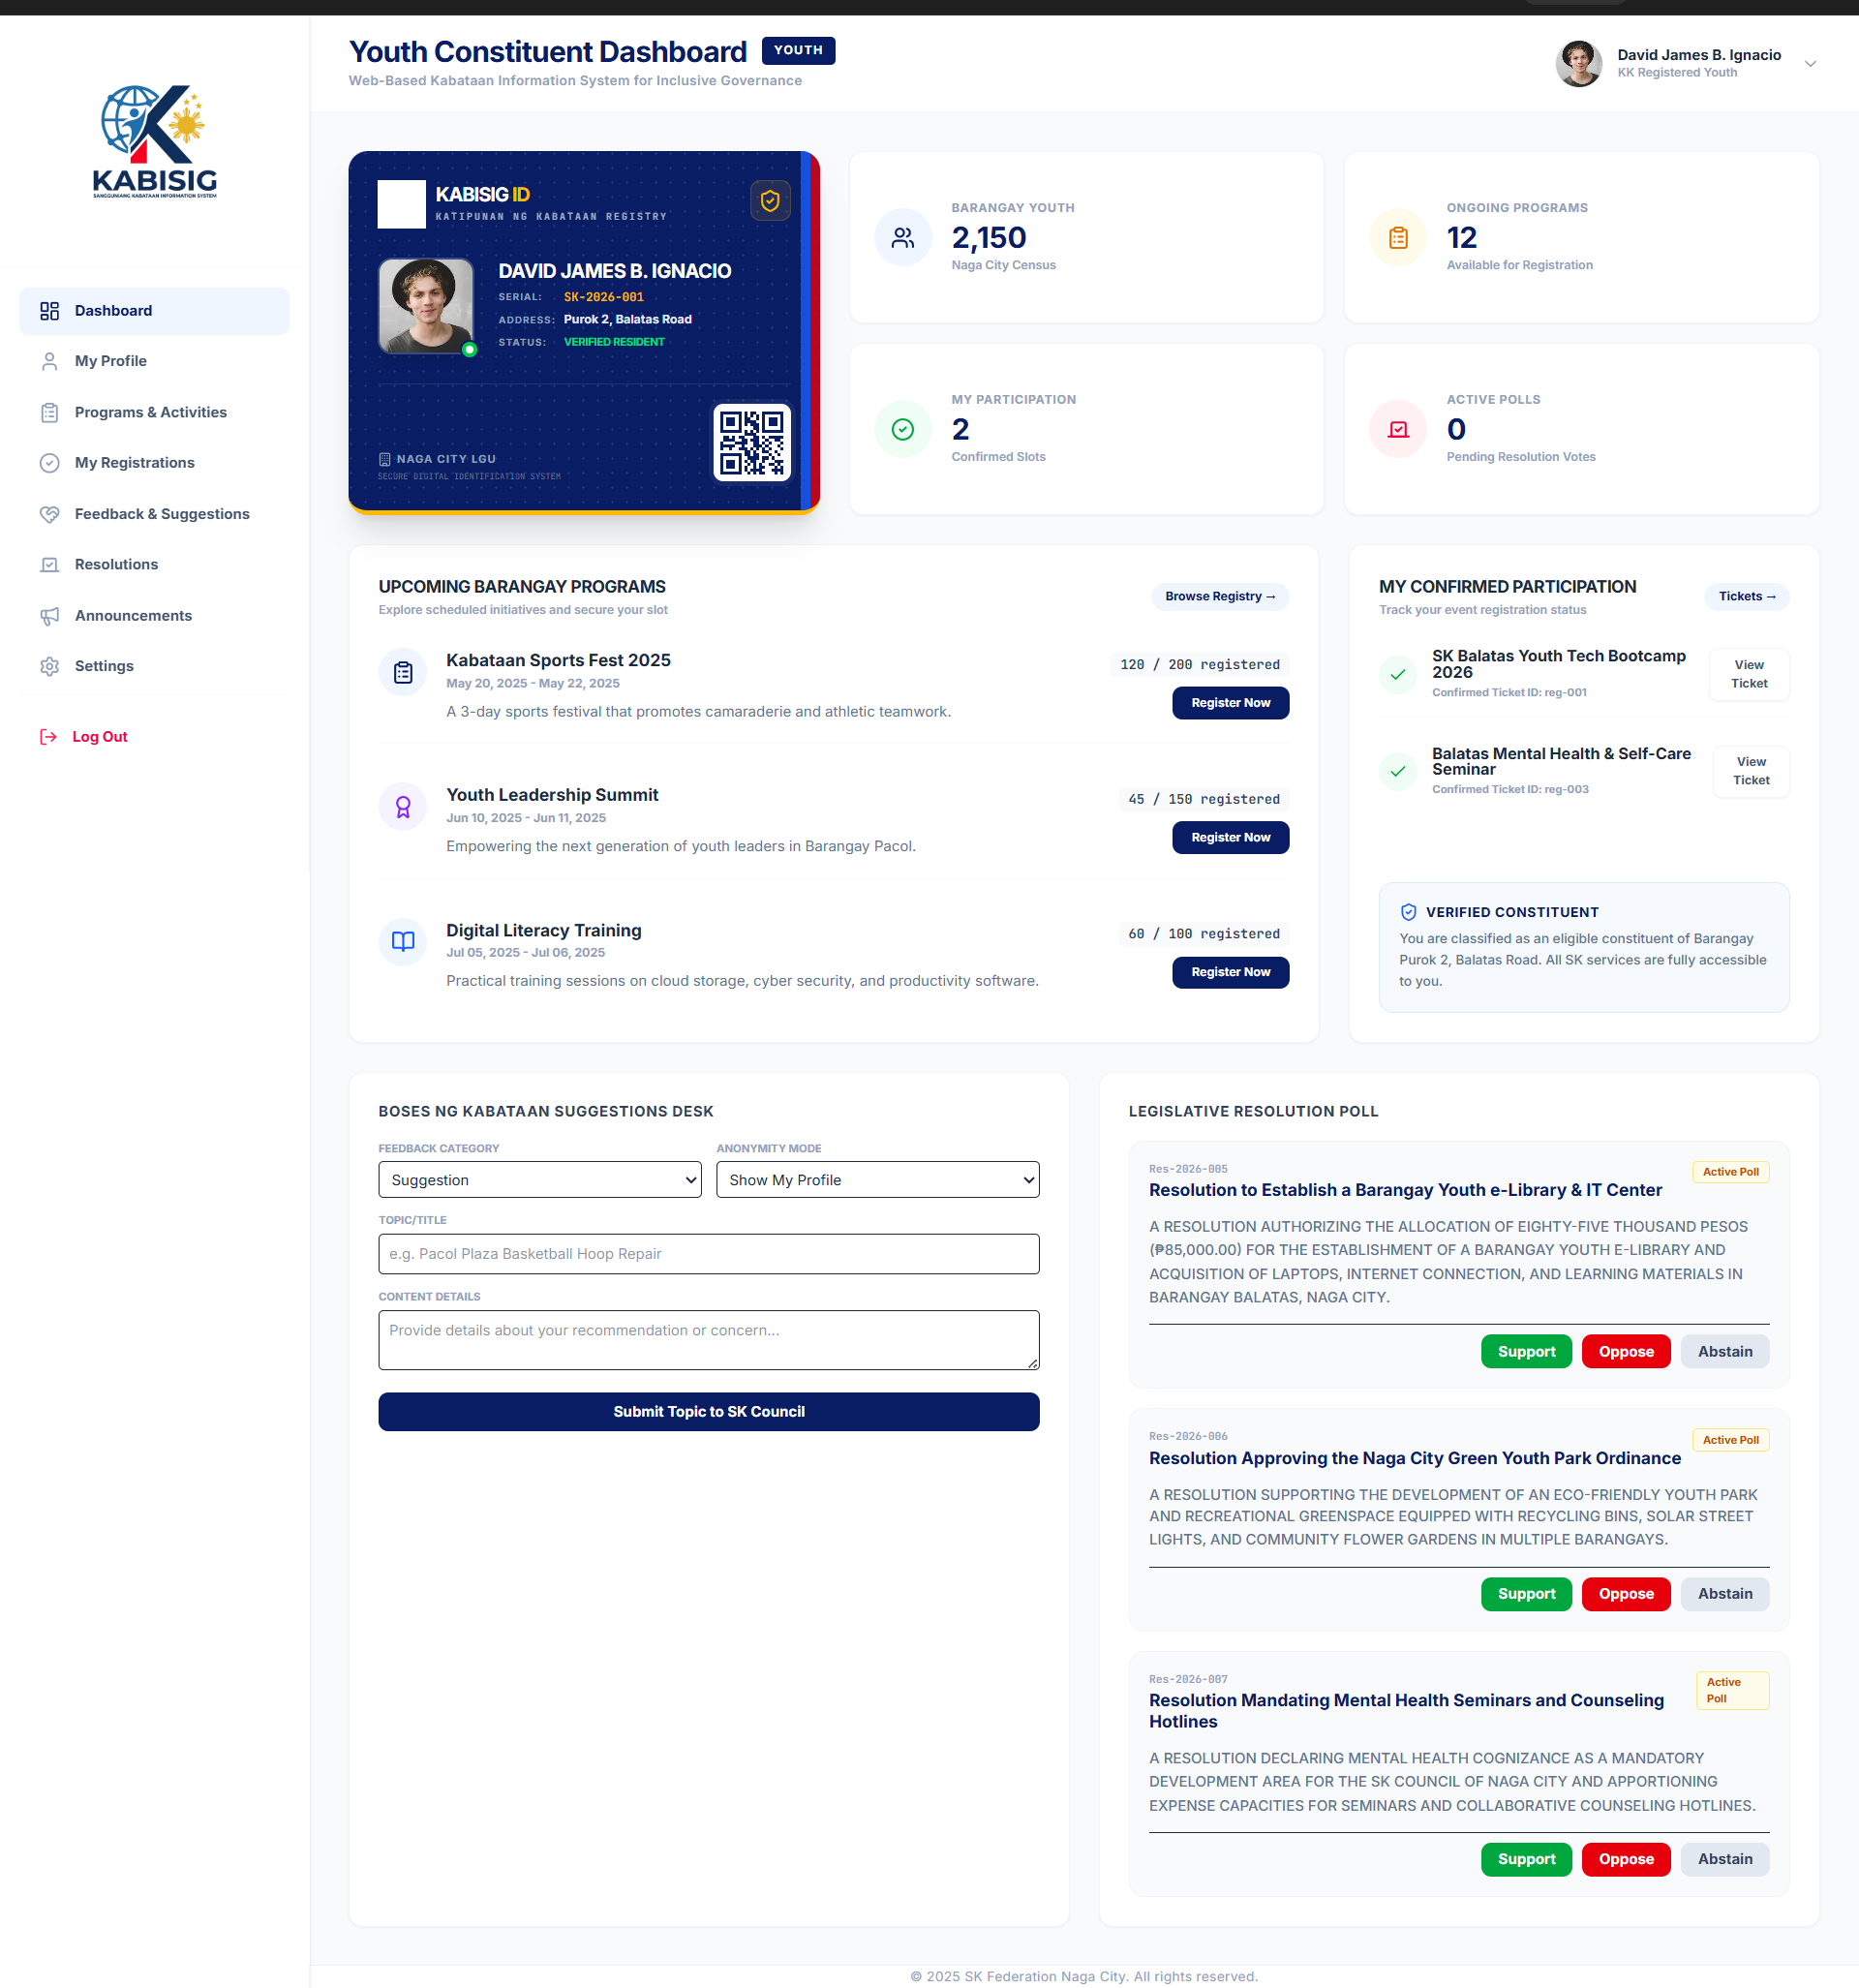
\includegraphics[width=0.45\textwidth]{figures/youth_dashboard.png}
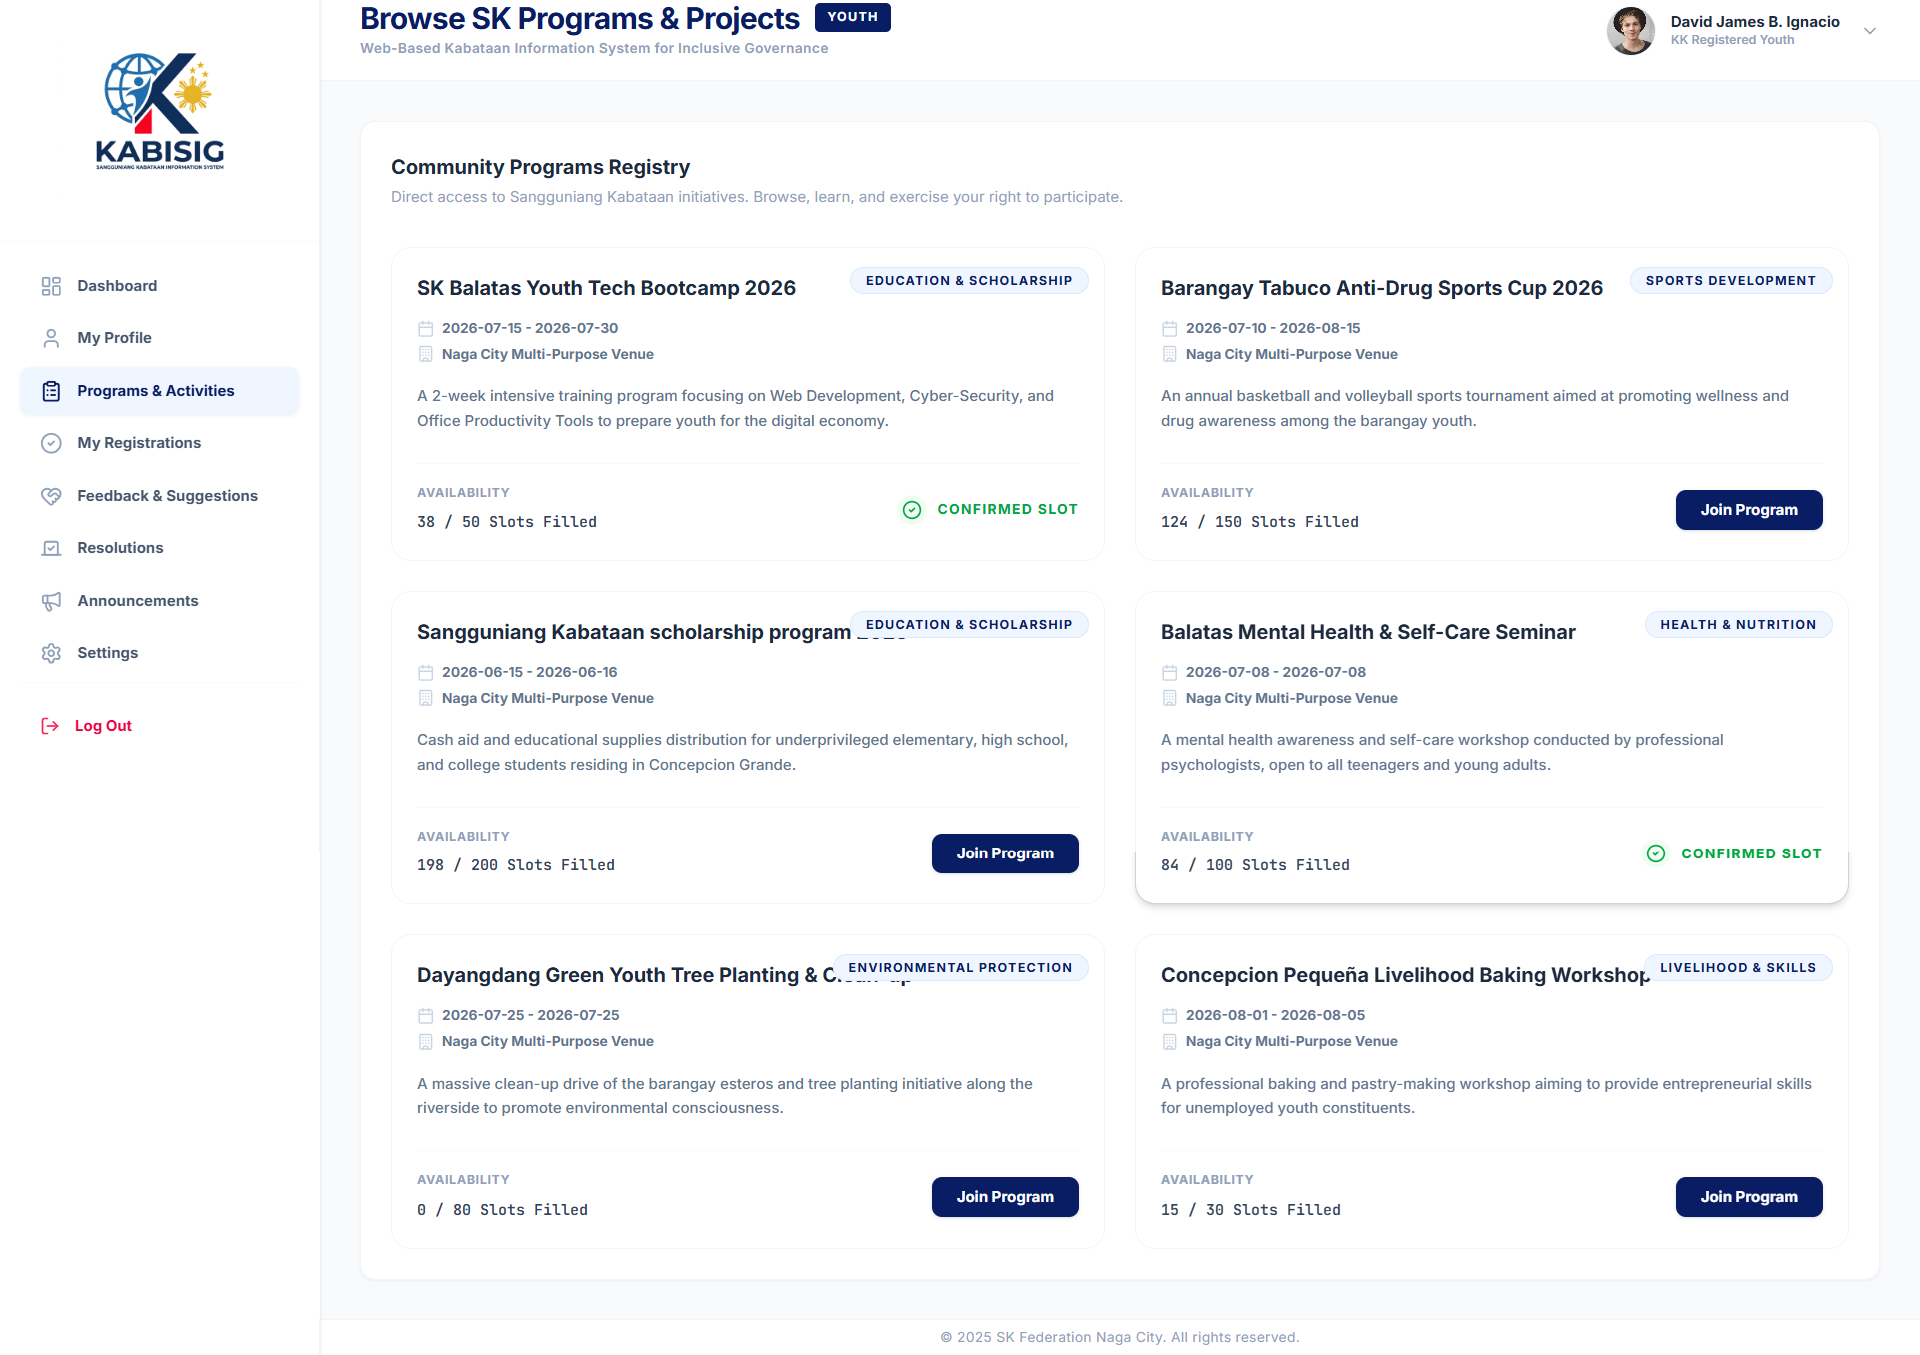
\includegraphics[width=0.45\textwidth]{figures/programs_browse.png}
\caption{Youth Dashboard and Program Browsing Screens (Sample Data)}
\label{fig:youth}
\end{figure}

\hspace*{\parindent} The Browse Programs screen displays available SK programs with details including title, category, date range, location, description, and slot availability. Youth can register for programs with a single click, and confirmed registrations are displayed in the My Confirmed Participation section.\vspace{5mm}

\hspace*{\parindent} The Boses ng Kabataan feedback module allows youth to submit suggestions, concerns, and inquiries to their SK Council. Users can select feedback categories, choose anonymity preferences, and track submission history with status updates and responses from SK officials.\vspace{5mm}

\begin{figure}[H]
\centering
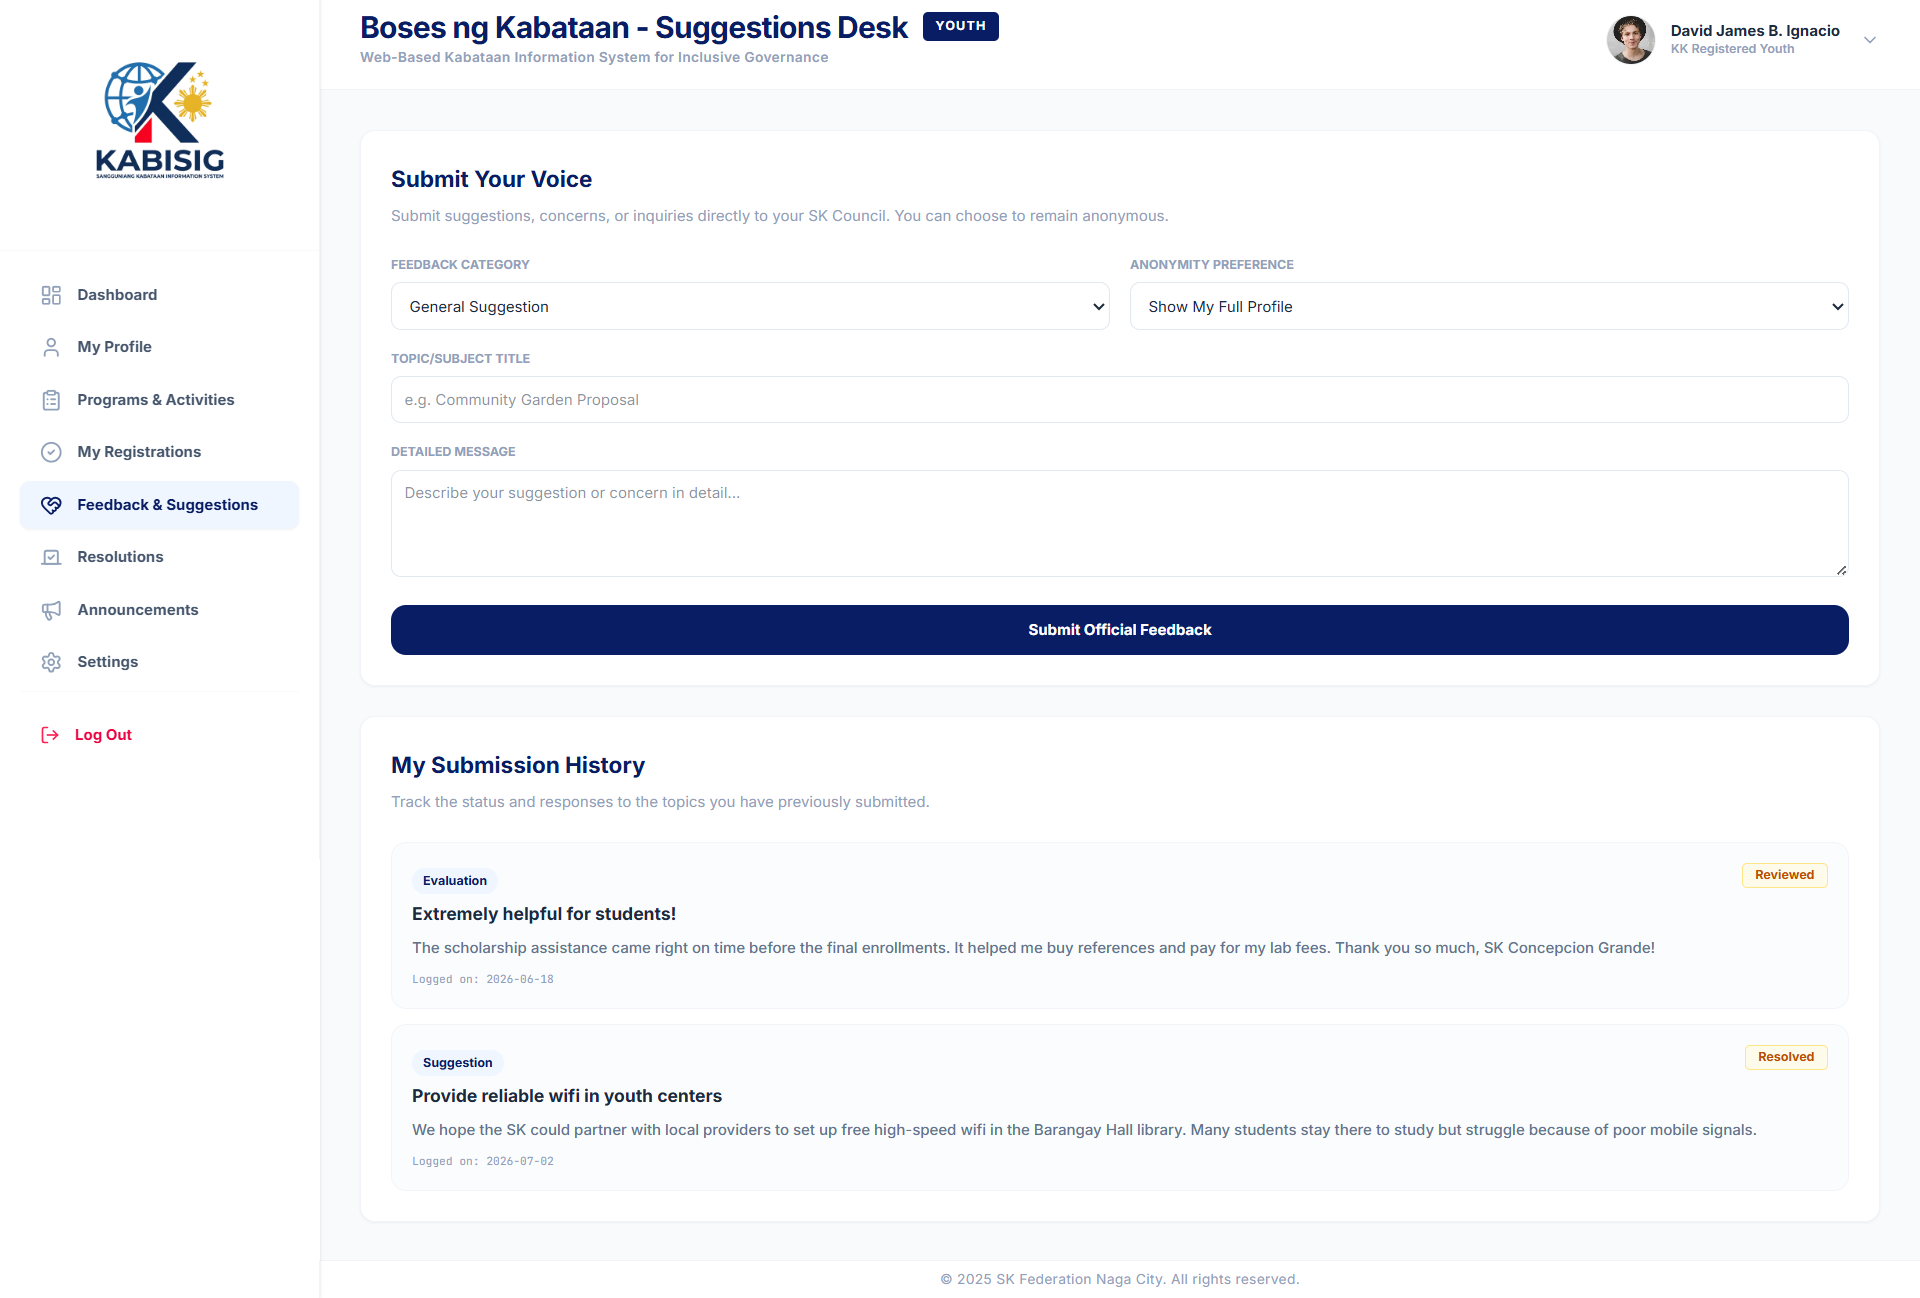
\includegraphics[width=0.45\textwidth]{figures/boses_ng_kabataan.png}
\caption{Boses ng Kabataan Feedback Module (Sample Data)}
\label{fig:feedback}
\end{figure}

\subsubsection{Mobile Responsive Design}

\hspace*{\parindent} All KABISIG screens are designed with a mobile-first approach, ensuring optimal usability on smartphones, tablets, and desktop devices. The interface features touch-friendly elements with minimum 44px touch targets, clear visual hierarchy, and intuitive navigation patterns. Users can efficiently access all system features through any modern web browser without requiring a native application download.\vspace{5mm}

\begin{figure}[H]
\centering
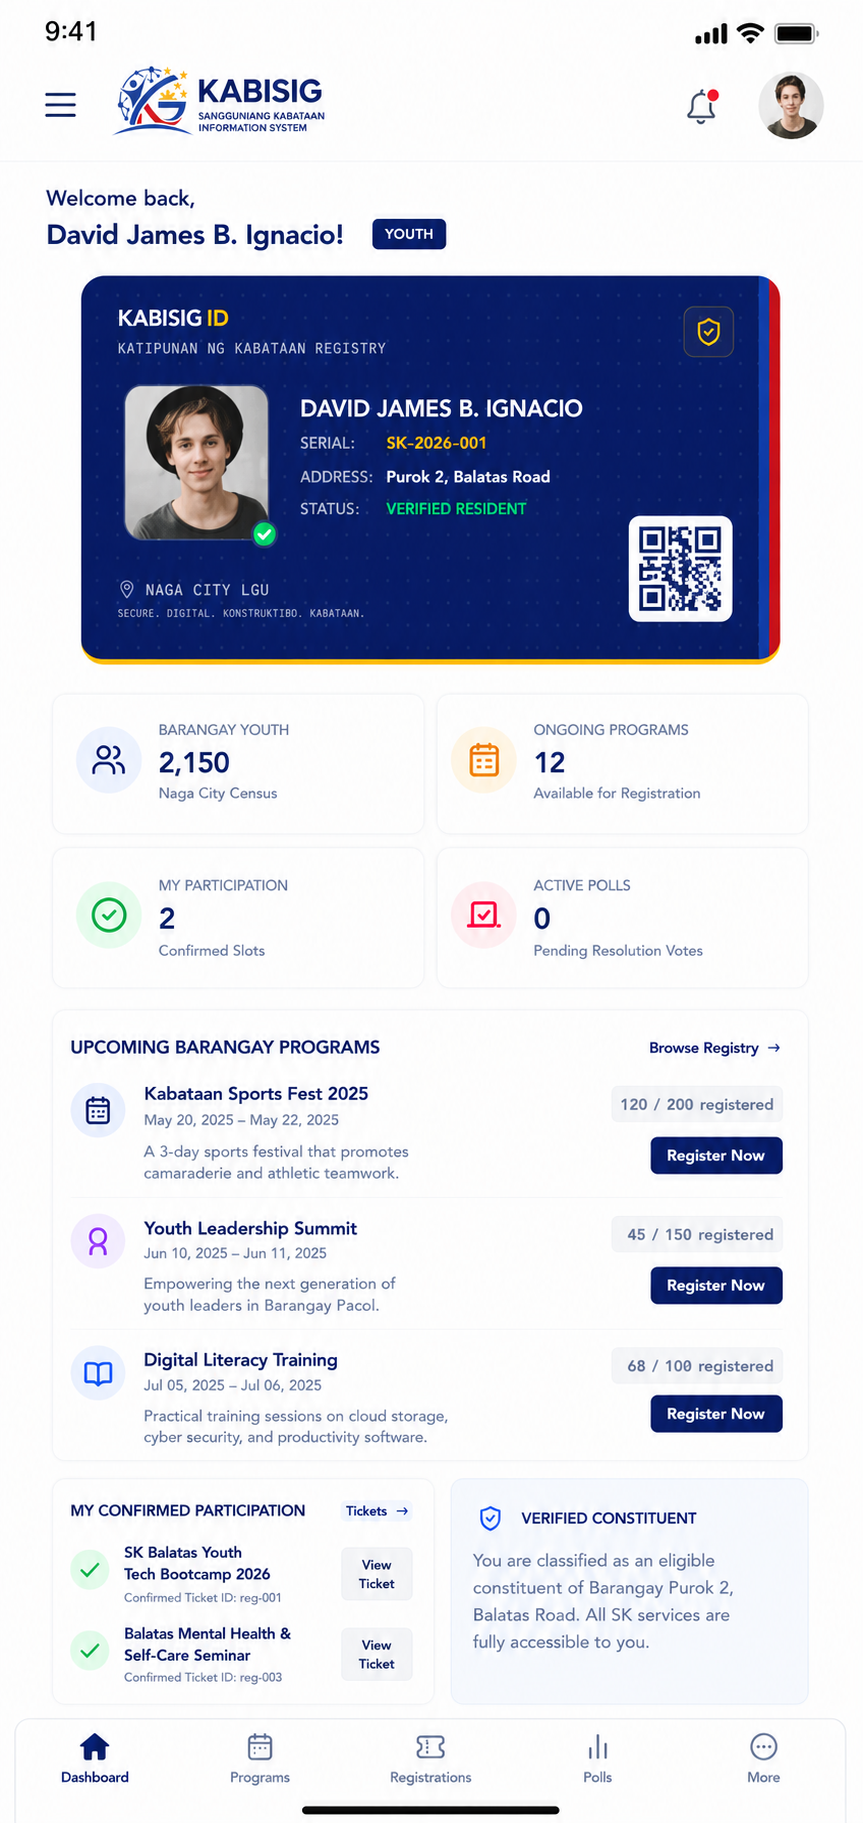
\includegraphics[width=0.30\textwidth]{figures/mobile_dashboard.png}
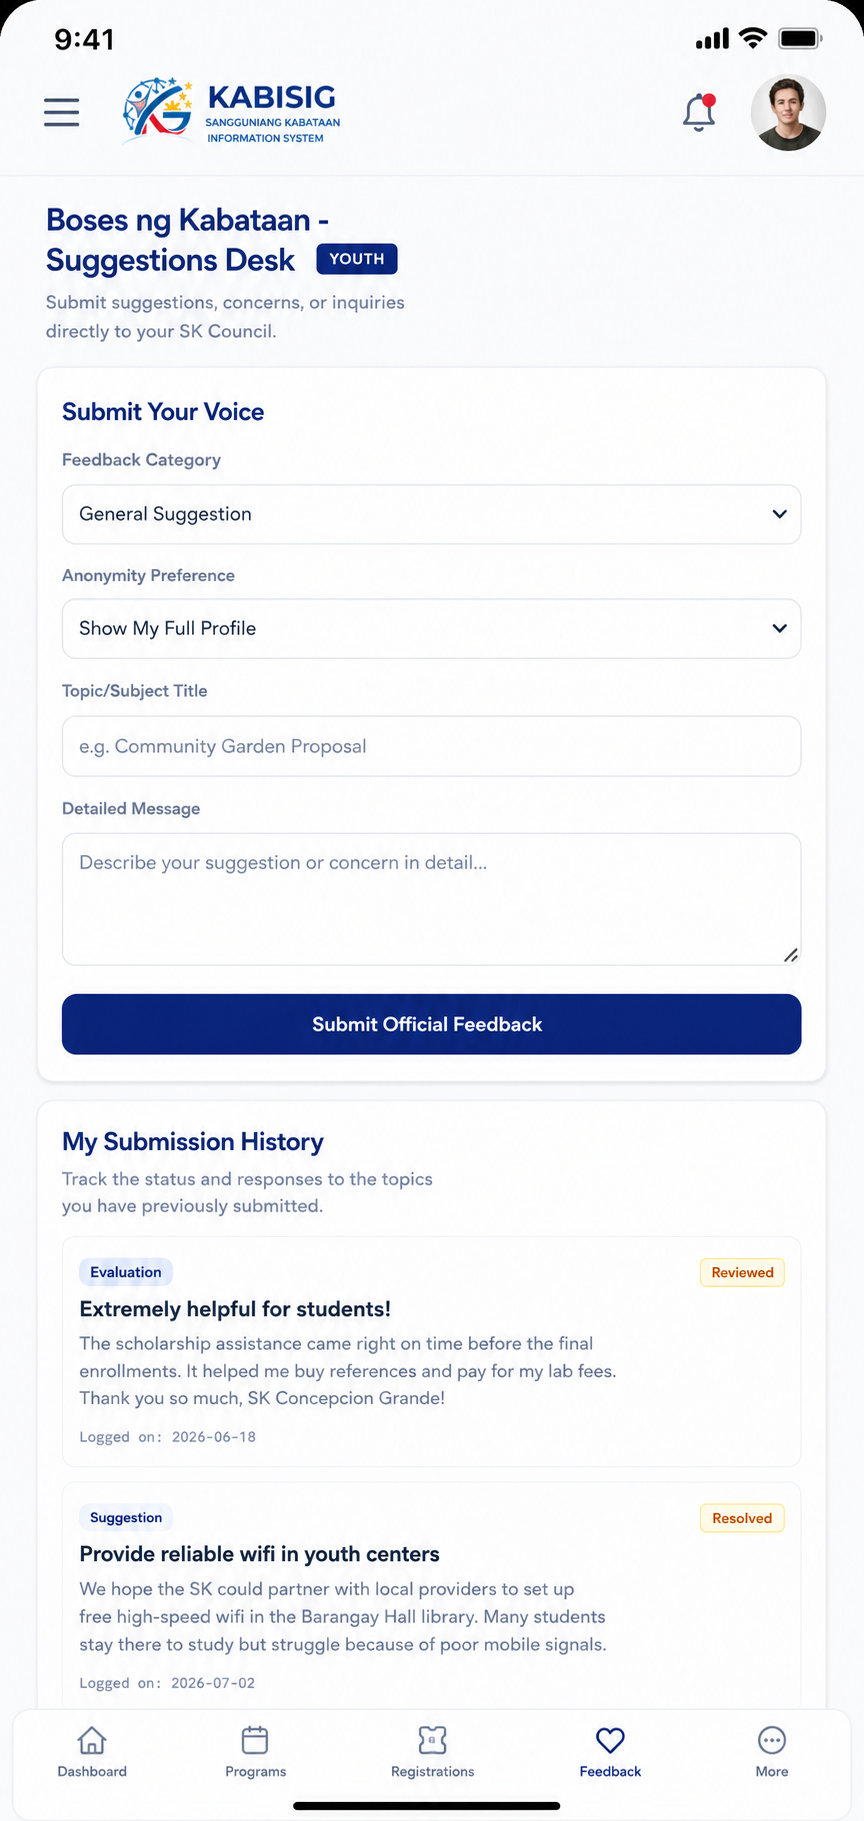
\includegraphics[width=0.30\textwidth]{figures/mobile_feedback.png}
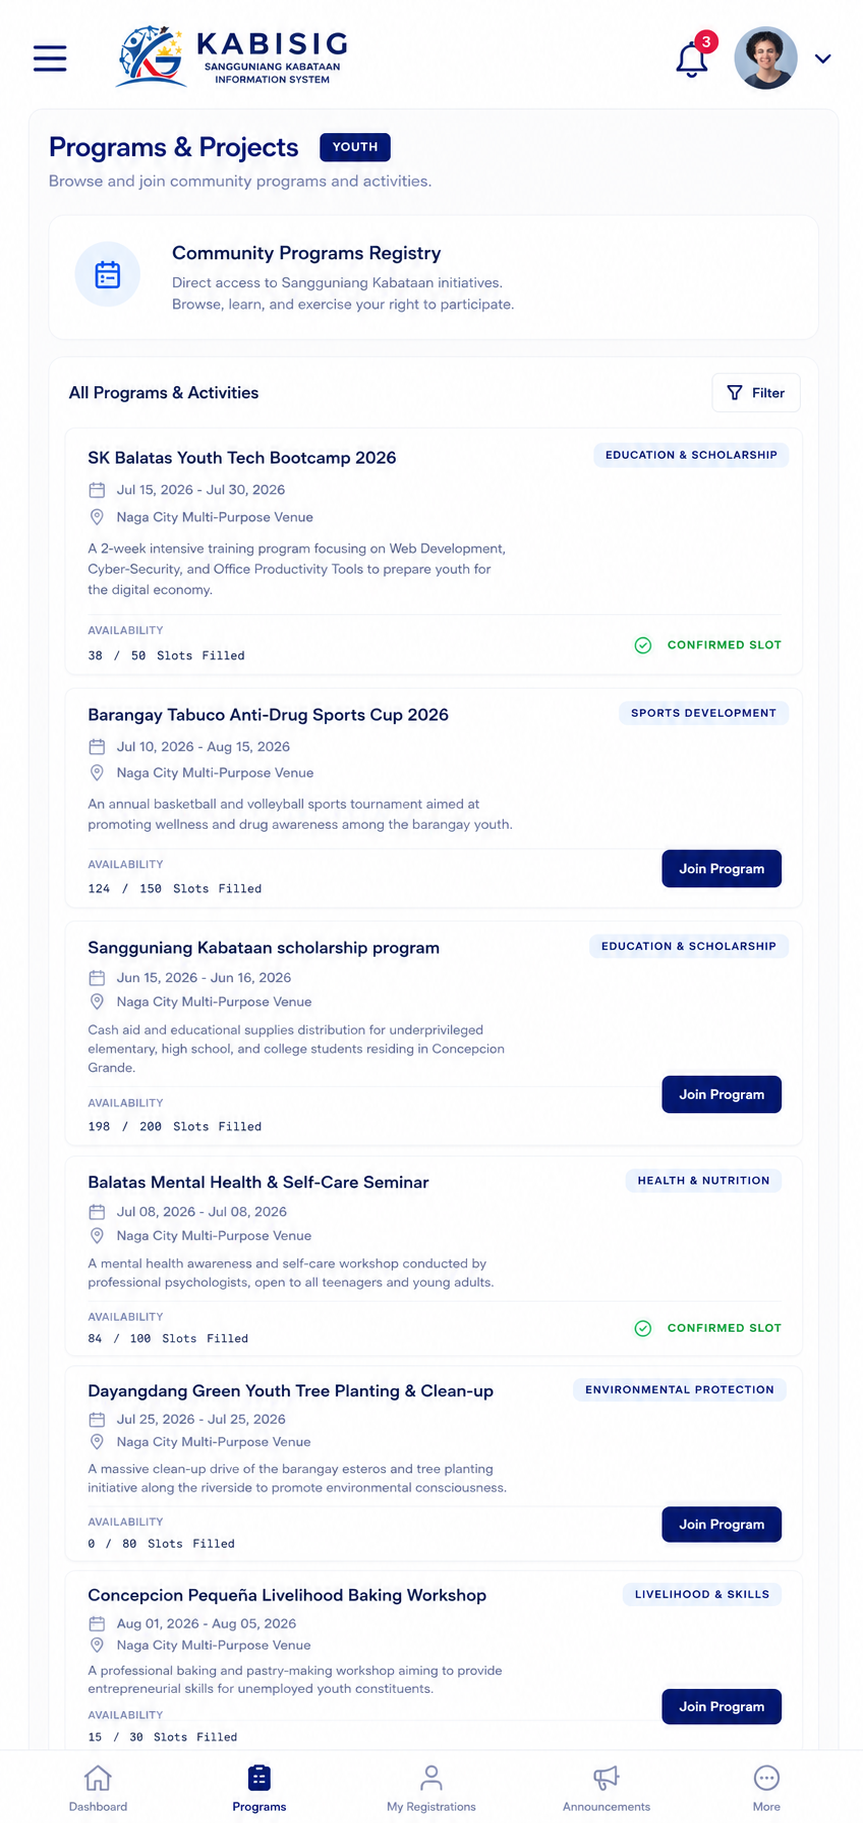
\includegraphics[width=0.30\textwidth]{figures/mobile_program.png}
\caption{Mobile Responsive Views of KABISIG Screens (Sample Data)}
\label{fig:mobile}
\end{figure}

\subsubsection{UI Components and Design System}

\hspace*{\parindent} The KABISIG design system includes reusable UI components that ensure consistency across all screens. These components include:\vspace{3mm}

\begin{itemize}
    \item \textbf{Cards:} White background with 12px border-radius, 16px padding, and subtle shadow for content display
    \item \textbf{Buttons:} Primary (Vibrant Red \#d32f2f), Secondary (Outline), and Text buttons with minimum 48px height for touch targets
    \item \textbf{Input Fields:} Light gray background with 8px border-radius, 14-16px padding, and clear labels
    \item \textbf{Badges:} Color-coded status indicators (Approved: Green, Pending: Yellow, Draft: Gray)
    \item \textbf{Navigation:} Bottom tab bar with icons and labels for mobile; left sidebar for desktop
    \item \textbf{Charts:} Clean, minimalist data visualizations using Recharts and D3.js
\end{itemize}

\vspace{5mm}

\begin{table}[H]
\centering
\caption{KABISIG Design System Color Palette}
\label{tab:colors}
\begin{tabular}{|l|c|l|}
\hline
\textbf{Color Name} & \textbf{Hex Code} & \textbf{Usage} \\
\hline
White & \#ffffff & Backgrounds, cards, text on dark \\
Light Gray & \#f5f5f5 & Section backgrounds, subtle separation \\
Deep Blue & \#1a237e & Headers, titles, primary text, active states \\
Vibrant Red & \#d32f2f & Primary action buttons, alerts, highlights \\
Gold & \#fdd835 & Accents, badges, highlights \\
Dark Text & \#212121 & Body text \\
Medium Text & \#616161 & Secondary text, labels \\
Light Text & \#9e9e9e & Placeholders, hints, subtle text \\
\hline
\end{tabular}
\end{table}

\subsubsection{Navigation Structure}

\hspace*{\parindent} Each user role has a tailored navigation structure that provides access to role-appropriate features and modules. The navigation adapts to screen size: bottom tab bar for mobile devices and left sidebar for tablet and desktop views. Active navigation items are highlighted with the KABISIG brand colors for clear orientation.\vspace{5mm}

\begin{table}[H]
\centering
\caption{KABISIG Navigation by User Role}
\label{tab:navigation}
\begin{tabular}{|>{\centering\arraybackslash}p{2.8cm}|>{\centering\arraybackslash}p{8cm}|}
\hline
\textbf{User Role} & \textbf{Navigation Items} \\
\hline
Super Admin & Dashboard, Barangays, Programs, Reports, More \\
\hline
Barangay Admin & Dashboard, Youth, Programs, Budget, Documents, Reports, Announcements, Social Sync, Calendar, Settings, Profile \\
\hline
SK Kagawad & Dashboard, Programs, Attendance, Resolutions, More \\
\hline
SK Secretary & Dashboard, Documents, Youth, Reports, More \\
\hline
SK Treasurer & Dashboard, Budget, Expenses, Inventory, More \\
\hline
Youth Constituent & Dashboard, Programs, Registrations, Feedback, More \\
\hline
Viewer & Home, Announcements, Transparency, Contact \\
\hline
\end{tabular}
\end{table}

\subsubsection{Accessibility Features}

\hspace*{\parindent} The KABISIG user interface incorporates accessibility features to ensure inclusive access for all users. These include:\vspace{3mm}

\begin{itemize}
    \item \textbf{High Contrast:} Text and background colors meet WCAG contrast ratio requirements
    \item \textbf{Screen Reader Support:} Semantic HTML and ARIA labels for assistive technologies
    \item \textbf{Touch Targets:} Minimum 44px touch targets for all interactive elements
    \item \textbf{Font Sizing:} Responsive typography that scales appropriately across devices
    \item \textbf{Color Blindness Support:} Status indicators use both color and icons for clarity
\end{itemize}

\vspace{5mm}

\hspace*{\parindent} The mobile-responsive design ensures that all KABISIG features remain fully functional and accessible on any device, supporting SK officials and youth constituents in their governance activities anytime, anywhere.\vspace{5mm}

